% Compilacion: usar la misma receta de LaTeX Workshop que los demas archivos.
% !TeX encoding = UTF-8
% ARCHIVO AUTONOMO: todos los graficos son vectoriales (TikZ/PGFPlots).
% MiKTeX + VS Code/LaTeX Workshop: compilar con pdfLaTeX dos veces,
% o con latexmk -pdf. No necesita imagenes, Python ni shell-escape.
% Paquetes estandar de MiKTeX. Si falta alguno, habilitar su instalacion.
% El idioma espanol se activa si babel-spanish esta instalado.
\documentclass[11pt,a4paper]{article}
\usepackage[utf8]{inputenc}
\usepackage[T1]{fontenc}
\usepackage{lmodern}
\IfFileExists{spanish.ldf}{\usepackage[spanish,es-nodecimaldot,es-noquoting]{babel}}{}
\usepackage[a4paper,margin=1.8cm,headheight=15pt]{geometry}
\usepackage{amsmath,amssymb,amsthm,mathtools,bm}
\usepackage{microtype,booktabs,array,longtable,multicol,enumitem}
\usepackage[dvipsnames]{xcolor}
\usepackage{tikz,pgfplots,tikz-3dplot}
\usetikzlibrary{arrows.meta,calc,angles,quotes,positioning,patterns,babel}
\usepgfplotslibrary{fillbetween,groupplots}
\pgfplotsset{compat=1.18}
\usepackage[most]{tcolorbox}
\usepackage{float,caption,fancyhdr}
\usepackage[colorlinks=true,linkcolor=MidnightBlue,urlcolor=MidnightBlue]{hyperref}
\hypersetup{pdftitle={PCA, teorema espectral, SVD y portafolios},pdfauthor={Tratado de estudio}}
\pdfstringdefDisableCommands{\def\ell{l}\def\infty{infinito}\def\to{ a }\def\norm#1{norma(#1)}\def\R{R}\def\N{N}}
\definecolor{azul}{RGB}{21,64,112}
\definecolor{celeste}{RGB}{235,244,252}
\definecolor{rojo}{RGB}{181,58,58}
\definecolor{verde}{RGB}{27,119,94}
\definecolor{gris}{RGB}{83,94,108}
\pagestyle{fancy}\fancyhf{}
\fancyhead[L]{\small\color{azul}PCA y teoría espectral}
\fancyhead[R]{\small\color{gris}Geometría, estadística, ML y portafolios}
\fancyfoot[C]{\small\thepage}
\setlength{\parindent}{0pt}\setlength{\parskip}{4pt}
\setlength{\abovedisplayskip}{6pt}\setlength{\belowdisplayskip}{6pt}
\setlength{\abovedisplayshortskip}{4pt}\setlength{\belowdisplayshortskip}{4pt}
\setlist{nosep,leftmargin=*}
\allowdisplaybreaks[2]
\emergencystretch=2em
\captionsetup{font=small,labelfont=bf,skip=5pt}
\renewcommand{\contentsname}{Índice}
\renewcommand{\figurename}{Figura}
\renewcommand{\tablename}{Cuadro}
\newcommand{\R}{\mathbb R}
\newcommand{\N}{\mathbb N}
\newcommand{\E}{\mathbb E}
\newcommand{\Prob}{\mathbb P}
\newcommand{\ind}{\mathbf 1}
\newcommand{\dd}{\,\mathrm d}
\newcommand{\T}{^{\mathsf T}}
\newcommand{\norm}[1]{\left\lVert #1\right\rVert}
\newcommand{\abs}[1]{\left\lvert #1\right\rvert}
\newcommand{\ip}[2]{\left\langle #1,#2\right\rangle}
\DeclareMathOperator{\Var}{Var}
\DeclareMathOperator{\Cov}{Cov}
\DeclareMathOperator{\Corr}{Corr}
\DeclareMathOperator{\spanop}{span}
\DeclareMathOperator{\esssup}{ess\,sup}
\DeclareMathOperator*{\argmin}{arg\,min}
\DeclareMathOperator{\sign}{sign}
\DeclareMathOperator{\tr}{tr}
\newtcolorbox{idea}[1][]{enhanced,breakable,colback=celeste,colframe=azul,boxrule=.5pt,arc=1mm,left=6pt,right=6pt,top=4pt,bottom=4pt,title={#1},fonttitle=\bfseries}
\newtcolorbox{ejemplo}[1][]{enhanced,breakable,colback=white,colframe=verde,boxrule=.5pt,arc=1mm,left=6pt,right=6pt,top=4pt,bottom=4pt,title={#1},fonttitle=\bfseries}
\newtcolorbox{cuidado}[1][]{enhanced,breakable,colback=red!2,colframe=rojo,boxrule=.5pt,arc=1mm,left=6pt,right=6pt,top=4pt,bottom=4pt,title={#1},fonttitle=\bfseries}
\newenvironment{deduccion}{\par\textbf{Deducción.}\ }{\hfill$\square$\par}
\pgfplotsset{base/.style={axis lines=middle,grid=both,minor tick num=1,grid style={gray!12},major grid style={gray!23},tick label style={font=\scriptsize},label style={font=\small},legend style={font=\scriptsize,draw=none,fill=white},samples=140},curva/.style={very thick,azul}}
\tikzset{vec/.style={-{Latex[length=2.6mm]},very thick,azul},vecrojo/.style={-{Latex[length=2.6mm]},very thick,rojo},vecverde/.style={-{Latex[length=2.6mm]},very thick,verde},eje/.style={-{Latex[length=1.8mm]},gray}}


\usepackage{listings,needspace}
\lstset{basicstyle=\ttfamily\footnotesize,breaklines=true,frame=single,rulecolor=\color{azul!40},backgroundcolor=\color{celeste!35},columns=fullflexible,keepspaces=true,showstringspaces=false}
\DeclareMathOperator{\rank}{rank}
\DeclareMathOperator{\diag}{diag}
\DeclareMathOperator{\kerop}{ker}
\DeclareMathOperator{\range}{Im}
\DeclareMathOperator*{\argmax}{arg\,max}
\newcommand{\Id}{I}
\newcommand{\F}{_{\mathrm F}}
\newcommand{\ones}{\mathbf 1}
\newcommand{\Sph}{\mathbb S}
\newtheorem{teorema}{Teorema}[section]
\newtheorem{proposicion}[teorema]{Proposición}
\newtheorem{lema}[teorema]{Lema}
\theoremstyle{definition}
\newtheorem{definicion}[teorema]{Definición}
\newcommand{\parte}[1]{\par\bigskip\Needspace{8\baselineskip}\begin{center}{\Large\bfseries\color{azul}#1}\end{center}}
\begin{document}
\begin{center}
{\Huge\bfseries\color{azul}PCA y reducción\\[3pt]de dimensionalidad}\\[7pt]
{\Large Autovectores, teorema espectral y SVD}\\[4pt]
{\large Geometría, demostraciones, aprendizaje automático y portafolios}\\[6pt]
\textit{Tratado de estudio: desde coordenadas y proyecciones hasta modelos avanzados.}
\end{center}
\begin{idea}[La identidad que organiza el tratado]
\[
\boxed{\underbrace{A}_{p\times p}\underbrace{v}_{p\times1}
=\underbrace{\lambda}_{1\times1}\underbrace{v}_{p\times1}}
\quad\Longrightarrow\quad
\boxed{AV=V\Lambda}\quad\Longrightarrow\quad
\boxed{A=V\Lambda V\T}\quad(A=A\T).
\]
Un autovector es una dirección que una transformación conserva; el autovalor mide el cambio de escala. Para una covarianza, esas direcciones son ejes de variabilidad. PCA conserva las de mayor varianza; la SVD permite calcularlas; la teoría de portafolios utiliza las mismas formas cuadráticas con restricciones diferentes.
\end{idea}
\textbf{Cómo estudiar.} Primero domina las partes I--III; rehace a mano los ejemplos de dos y tres variables; después estudia SVD, regresión y portafolios. Las partes avanzadas explican qué cambia al usar métricas, núcleos, variables latentes o funciones. Las demostraciones de los resultados centrales son explícitas; cuando una extensión solo se presenta o se bosqueja, se indica.

\textbf{Contrato de notación.} Trabajamos sobre $\R$, salvo una observación expresa sobre $\mathbb C$. Los vectores son columnas, escritos habitualmente como transpuestos para ahorrar espacio. $n\ge2$ es el número de observaciones, $p$ el número de variables, $r$ el rango de la matriz centrada y $k$ la dimensión conservada, $1\le k\le r$. La letra $X$ designa datos; $A$ una transformación cuadrada; $S$ la covarianza muestral; $\Sigma$ la poblacional. No se confunden datos, ejes, puntuaciones ni pesos financieros.

\textbf{Formato y compilación.} Documento autónomo: todas las figuras están dibujadas en TikZ/PGFPlots dentro de este mismo archivo. Compilar con pdfLaTeX dos veces o con \texttt{latexmk -pdf}. No requiere imágenes externas, Python, \texttt{shell-escape} ni cambios en la configuración de VS Code. Las instrucciones y el ejemplo MATLAB están al final.

\setcounter{tocdepth}{1}
\section*{Índice de la ruta completa}
\begin{multicols}{2}\footnotesize\setlength{\parskip}{0pt}
\makeatletter
\renewcommand*\l@section[2]{\@dottedtocline{1}{0pt}{1.9em}{#1}{#2}}
\@starttoc{toc}
\makeatother
\end{multicols}

\parte{I. Geometría y álgebra: entender qué significa una dirección}
\section{Dimensión, coordenadas y la necesidad de reducir}
Una observación con $p$ características es $x_i=(x_{i1},\ldots,x_{ip})\T\in\R^{p\times1}$. Por ejemplo, tres mediciones de una persona forman un vector en $\R^3$; no es necesario que las coordenadas sean posiciones físicas. La dimensión ambiente es $p$; la estructura efectiva puede ocupar menos dimensiones.
\begin{ejemplo}[Tres columnas, una sola fuente de variación]
Para $t_i\in\R$, sea $x_i=(t_i,2t_i,3t_i)\T\in\R^{3\times1}$. Aunque registramos tres variables,
\[
x_i=t_i a,\quad a=(1,2,3)\T\in\R^{3\times1},\qquad
\spanop\{a\}=\{ta:t\in\R\}.
\]
Todos los puntos pertenecen a una recta: dimensión lineal uno. Con ruido $\varepsilon_i\in\R^{3\times1}$, $x_i=t_i a+\varepsilon_i$ ya puede tener rango tres, pero seguir cerca de esa recta. PCA busca una aproximación, no una dependencia exacta obligatoria.
\end{ejemplo}
\subsection{Selección frente a extracción de características}
Seleccionar elige columnas originales, por ejemplo $(x_{i1},x_{i3})\T\in\R^{2\times1}$. Extraer construye combinaciones $z_i=W\T x_i\in\R^{k\times1}$, con $W\in\R^{p\times k}$. PCA es extracción lineal. La reconstrucción $Wz_i\in\R^{p\times1}$ vuelve al espacio original, pero normalmente pierde información.
\[
\underbrace{x_i}_{p\times1}\ \xrightarrow{\ W\T\ }\
\underbrace{z_i}_{k\times1}\ \xrightarrow{\ W\ }\
\underbrace{\widehat x_i}_{p\times1},\qquad k<p.
\]
\subsection{Por qué muchas variables pueden ser un problema}
Una cuadrícula con $m$ posiciones por variable tiene $m^p$ celdas. Con $m=10$, dos variables producen $100$ celdas; diez producen $10^{10}$. Eso ilustra la dificultad de cubrir el espacio. Además, muchas columnas correlacionadas pueden volver inestable una regresión. PCA ayuda cuando una estructura de baja dimensión explica la variación relevante, pero no garantiza que esa variación sea útil para predecir una respuesta.
\begin{cuidado}[Tres dimensiones que no son lo mismo]
La dimensión ambiente $p$, el rango algebraico $r$ y una dimensión intrínseca no lineal son conceptos diferentes. Un círculo en $\R^2$ tiene dimensión intrínseca uno, pero su nube centrada suele tener rango dos. Ninguna recta reconstruye exactamente todo el círculo.
\end{cuidado}

\section{Matrices, productos y formas cuadráticas sin operaciones ocultas}
Sea $A=(a_{ij})\in\R^{p\times p}$ y $v=(v_1,\ldots,v_p)\T\in\R^{p\times1}$:
\[
A=\begin{pmatrix}a_{11}&a_{12}&\cdots&a_{1p}\\a_{21}&a_{22}&\cdots&a_{2p}\\\vdots&\vdots&\ddots&\vdots\\a_{p1}&a_{p2}&\cdots&a_{pp}\end{pmatrix},\qquad
Av=\begin{pmatrix}\sum_{j=1}^pa_{1j}v_j\\\sum_{j=1}^pa_{2j}v_j\\\vdots\\\sum_{j=1}^pa_{pj}v_j\end{pmatrix}\in\R^{p\times1}.
\]
El producto interno es $u\T v=\sum_j u_jv_j\in\R$ y el producto exterior es $uv\T=(u_iv_j)_{ij}\in\R^{p\times p}$, para $u,v\in\R^{p\times1}$. No son intercambiables.
\[
\norm v_2^2=v\T v,\qquad v\T Av=\sum_{i=1}^p\sum_{j=1}^pa_{ij}v_iv_j\in\R.
\]
Para $A=\begin{psmallmatrix}a&b\\b&c\end{psmallmatrix}$ y $v=(s,t)\T\in\R^{2\times1}$,
\[
v\T Av=as^2+2bst+ct^2,\qquad
\nabla_v(v\T Av)=\begin{pmatrix}2as+2bt\\2bs+2ct\end{pmatrix}=2Av.
\]
En general, derivando coordenada por coordenada,
\[
\frac{\partial}{\partial v_\ell}\sum_{i,j}a_{ij}v_iv_j
=\sum_j a_{\ell j}v_j+\sum_i a_{i\ell}v_i,
\quad \nabla_v(v\T Av)=(A+A\T)v.
\]
Así, $2Av$ requiere simetría. La Hessiana es $2A$ cuando $A=A\T$.
\subsection{Traza y norma de Frobenius}
Para $B=(b_{ij})\in\R^{n\times p}$,
\[
\norm B\F^2=\sum_{i=1}^n\sum_{j=1}^pb_{ij}^2=\tr(B\T B),\qquad
\tr(CD)=\tr(DC),
\]
si $C\in\R^{a\times b}$ y $D\in\R^{b\times a}$. La última igualdad resulta de sumar $\sum_i\sum_j c_{ij}d_{ji}$ en distinto orden. La traza no autoriza permutar factores arbitrariamente: permite rotaciones cíclicas compatibles.
\begin{ejemplo}[Una multiplicación que reaparecerá en PCA]
\[
A=\begin{pmatrix}3&1\\1&3\end{pmatrix},\quad
v=\frac1{\sqrt2}(1,1)\T,\quad
Av=\frac1{\sqrt2}(4,4)\T=4v,\quad v\T Av=4.
\]
Para $u=(1,0)\T$, $Au=(3,1)\T$ no es múltiplo de $u$, y $u\T Au=3$. Ambas direcciones son unitarias, pero la primera recibe mayor valor de la forma cuadrática.
\end{ejemplo}

\section{Bases ortonormales, proyecciones y Pitágoras matricial}
Una familia $v_1,\ldots,v_k\in\R^{p\times1}$ es ortonormal si $v_i\T v_j=\delta_{ij}$, donde $\delta_{ij}$ vale uno si $i=j$ y cero en otro caso. La matriz $V_k=[v_1\ \cdots\ v_k]\in\R^{p\times k}$ satisface $V_k\T V_k=I_k$.
\begin{teorema}[Proyección sobre un subespacio]
Para $x\in\R^{p\times1}$, el punto de $\range(V_k)$ más cercano a $x$ es
\[
\widehat x=V_kV_k\T x,\qquad P_k=V_kV_k\T\in\R^{p\times p},\qquad
P_k\T=P_k,\quad P_k^2=P_k.
\]
\end{teorema}
\begin{deduccion}
Cualquier candidato es $V_k a$, con $a\in\R^{k\times1}$. Expandiendo,
\[
\norm{x-V_ka}_2^2=x\T x-2a\T V_k\T x+a\T a
=\norm{x}_2^2-\norm{V_k\T x}_2^2+\norm{a-V_k\T x}_2^2.
\]
El único mínimo en coordenadas es $a=V_k\T x$. Además,
\[
V_k\T(x-\widehat x)=V_k\T x-I_kV_k\T x=0,\qquad
\norm x_2^2=\norm{\widehat x}_2^2+\norm{x-\widehat x}_2^2.
\]
La simetría e idempotencia se verifican multiplicando $P_k$ y usando $V_k\T V_k=I_k$.
\end{deduccion}
\begin{ejemplo}[Una dirección, una coordenada y una proyección]
Sean $x=(3,1)\T\in\R^{2\times1}$ y $v=(1,1)\T/\sqrt2\in\R^{2\times1}$. Entonces
\[
z=v\T x=2\sqrt2\in\R,\quad \widehat x=zv=(2,2)\T,\quad e=x-\widehat x=(1,-1)\T,
\]
\[
P=vv\T=\frac12\begin{pmatrix}1&1\\1&1\end{pmatrix},\quad
v\T e=0,\quad \norm x_2^2=10=8+2=\norm{\widehat x}_2^2+\norm e_2^2.
\]
$z$ es un escalar; $\widehat x$ es un vector. Confundirlos oculta el significado de reducir y reconstruir.
\end{ejemplo}
\begin{figure}[H]\centering
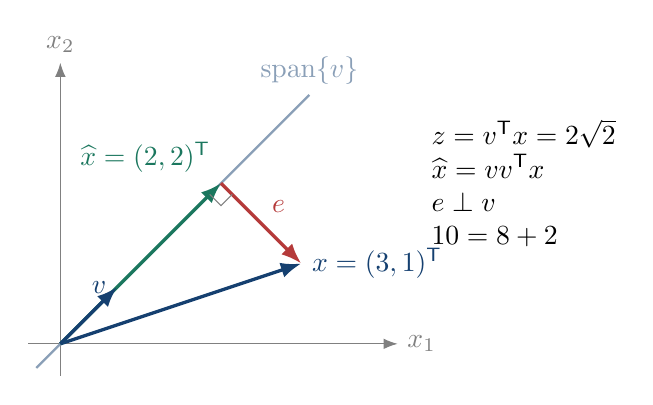
\begin{tikzpicture}[scale=1.02]
\draw[eje](-.4,0)--(4.2,0)node[right]{$x_1$};\draw[eje](0,-.4)--(0,3.5)node[above]{$x_2$};
\draw[azul!50,thick](-.3,-.3)--(3.1,3.1)node[above]{$\spanop\{v\}$};
\draw[vec](0,0)--(3,1)node[right]{$x=(3,1)\T$};
\draw[vecverde](0,0)--(2,2)node[above left]{$\widehat x=(2,2)\T$};
\draw[vecrojo](2,2)--(3,1)node[midway,above right]{$e$};
\draw[vec](0,0)--(.707,.707)node[left]{$v$};
\draw[gray](1.86,1.86)--(2,1.72)--(2.14,1.86);
\node[align=left,anchor=west]at(4.5,2){$z=v\T x=2\sqrt2$\\$\widehat x=vv\T x$\\$e\perp v$\\$10=8+2$};
\end{tikzpicture}
\caption{La coordenada $z$ mide cuánto avanzar sobre el eje unitario; el residuo es perpendicular a la recta.}
\end{figure}
\subsection{Cambiar toda la base no reduce dimensión}
Si $V\in\R^{p\times p}$ es ortogonal, $V\T V=VV\T=I_p$. Para $z=V\T x$, $x=Vz$ y $\norm z_2=\norm x_2$. La rotación o reflexión conserva toda la información. La reducción aparece al descartar coordenadas, usando $V_k\T\in\R^{k\times p}$ con $k<p$.

\section{Autovalores y autovectores: definición y cálculo completo}
\begin{definicion}
Para $A\in\R^{p\times p}$, un escalar $\lambda$ es autovalor si existe $v\in\R^{p\times1}\setminus\{0\}$ tal que $Av=\lambda v$. El vector $v$ es un autovector y
\[
E_\lambda=\kerop(A-\lambda I_p)=\{v:(A-\lambda I_p)v=0\}
\]
es el autoespacio asociado, incluyendo el vector cero como elemento del subespacio.
\end{definicion}
La igualdad significa que $Av$ permanece en la recta de $v$. Si $\lambda>1$, estira; si $0<\lambda<1$, contrae; si $\lambda<0$, invierte el sentido; si $\lambda=0$, anula la dirección. El vector cero no define una dirección y por eso no se llama autovector.
\subsection{Por qué aparece el determinante}
El sistema homogéneo $(A-\lambda I_p)v=0$ tiene solución no nula exactamente cuando su matriz es singular:
\[
\boxed{\det(A-\lambda I_p)=0.}
\]
Se calculan primero las raíces y luego cada núcleo; el determinante no proporciona por sí solo los autovectores. Multiplicar un autovector por cualquier escalar no nulo produce otro; su longitud se fija normalizando y su signo permanece convencional.
\begin{ejemplo}[Resolución exacta de una matriz simétrica]
Para $A=\begin{psmallmatrix}3&1\\1&3\end{psmallmatrix}\in\R^{2\times2}$,
\[
\det(A-\lambda I_2)=(3-\lambda)^2-1=\lambda^2-6\lambda+8
=(\lambda-4)(\lambda-2).
\]
Para $\lambda_1=4$, $-v_1+v_2=0$, luego tomamos $(1,1)\T$ y normalizamos. Para $\lambda_2=2$, $v_1+v_2=0$, luego tomamos $(1,-1)\T$:
\[
v_1=\frac1{\sqrt2}(1,1)\T,\quad v_2=\frac1{\sqrt2}(1,-1)\T,\quad
V=\frac1{\sqrt2}\begin{pmatrix}1&1\\1&-1\end{pmatrix},\quad
\Lambda=\begin{pmatrix}4&0\\0&2\end{pmatrix}.
\]
Ambos $v_j\in\R^{2\times1}$; $V,\Lambda\in\R^{2\times2}$; $V\T V=I_2$. Finalmente,
\[
AV=[Av_1\ Av_2]=[4v_1\ 2v_2]=V\Lambda,
\quad A=V\Lambda V\T=4v_1v_1\T+2v_2v_2\T.
\]
\end{ejemplo}
\subsection{Multiplicidad y casos donde la diagonalización falla}
La multiplicidad algebraica cuenta cuántas veces aparece una raíz del polinomio característico; la geométrica es $\dim E_\lambda$. Una matriz es diagonalizable si admite $p$ autovectores linealmente independientes.
\[
J=\begin{pmatrix}1&1\\0&1\end{pmatrix}:\quad
\det(J-\lambda I_2)=(1-\lambda)^2,\quad E_1=\spanop\{(1,0)\T\}.
\]
Tiene multiplicidad algebraica dos y geométrica uno; no es diagonalizable. En cambio, $A=3I_2$ tiene un solo autovalor distinto, pero \emph{toda} base ortonormal es una base de autovectores. Autovalores repetidos no implican fracaso.
\begin{cuidado}[Simetría no es un adorno]
Una matriz real puede no tener autovectores reales: la rotación $R=\begin{psmallmatrix}0&-1\\1&0\end{psmallmatrix}$ cumple $\lambda^2+1=0$. Su diagonalización requiere $\mathbb C$. Para covarianzas reales, la simetría elimina estas dificultades y garantiza una base ortonormal real.
\end{cuidado}

\section{Teorema espectral real: demostración desde la esfera}
\begin{teorema}[Teorema espectral]
Si $A=A\T\in\R^{p\times p}$, existen una matriz ortogonal $V=[v_1\ \cdots\ v_p]\in\R^{p\times p}$ y una diagonal real $\Lambda=\diag(\lambda_1,\ldots,\lambda_p)$ tales que
\[
\boxed{A=V\Lambda V\T=\sum_{j=1}^p\lambda_jv_jv_j\T},\qquad
Av_j=\lambda_jv_j,\qquad v_i\T v_j=\delta_{ij}.
\]
\end{teorema}
\begin{deduccion}
\textbf{1. Existe una dirección extrema.} La esfera $\Sph^{p-1}=\{v\in\R^{p\times1}:v\T v=1\}$ es compacta y $f(v)=v\T Av$ es continua; por tanto tiene máximo en algún $v_1$. Para cualquier $h\perp v_1$, $h\in\R^{p\times1}$, considera
\[
g(t)=\frac{(v_1+th)\T A(v_1+th)}{\norm{v_1+th}_2^2}.
\]
Como $t=0$ maximiza localmente, $g'(0)=2h\T Av_1=0$. Esto vale para todo $h\perp v_1$, por lo que $Av_1$ es paralelo a $v_1$: $Av_1=\lambda_1v_1$, con $\lambda_1=v_1\T Av_1\in\R$.

\textbf{2. El complemento ortogonal es invariante.} Si $u\in\R^{p\times1}$ y $v_1\T u=0$, entonces
\[
v_1\T Au=(Av_1)\T u=\lambda_1v_1\T u=0.
\]
Así, $A$ envía $v_1^\perp$ a sí mismo. En cualquier base ortonormal de ese subespacio de dimensión $p-1$, su restricción sigue siendo simétrica.

\textbf{3. Inducción.} El caso $p=1$ es inmediato. Aplicando el mismo argumento a la restricción obtenemos $p-1$ autovectores ortonormales dentro de $v_1^\perp$. Junto con $v_1$ forman la base requerida. De $AV=V\Lambda$ y $VV\T=I_p$ se deduce $A=V\Lambda V\T$.
\end{deduccion}
\subsection{Ortogonalidad para autovalores distintos}
Si $Av_i=\lambda_iv_i$ y $Av_j=\lambda_jv_j$,
\[
\lambda_i v_i\T v_j=(Av_i)\T v_j=v_i\T Av_j
=\lambda_jv_i\T v_j
\quad\Rightarrow\quad(\lambda_i-\lambda_j)v_i\T v_j=0.
\]
Si $\lambda_i\ne\lambda_j$, $v_i\T v_j=0$. Dentro de un autoespacio repetido, Gram--Schmidt produce una base ortonormal sin salir del autoespacio.
\subsection{Consecuencias que usaremos continuamente}
Para $a=V\T x\in\R^{p\times1}$ y $x\in\R^{p\times1}$,
\[
x\T Ax=a\T\Lambda a=\sum_j\lambda_ja_j^2,\quad
\tr A=\sum_j\lambda_j,\quad \det A=\prod_j\lambda_j,\quad
\rank A=\#\{j:\lambda_j\ne0\}.
\]
$A$ es semidefinida positiva, escrito $A\succeq0$, si $x\T Ax\ge0$ para todo $x$; equivale a $\lambda_j\ge0$ para todos los $j$. Es definida positiva, $A\succ0$, si todos son estrictamente positivos.
\[
A^{-1}=V\diag(\lambda_j^{-1})V\T\quad(\lambda_j\ne0),\qquad
A^{1/2}=V\diag(\sqrt{\lambda_j})V\T\quad(A\succeq0).
\]
Estas expresiones se comprueban multiplicando y cancelando $V\T V$. La raíz escrita es la única raíz simétrica semidefinida positiva; no se afirma que toda raíz matricial sea única.
\begin{idea}[Lectura geométrica de la descomposición]
$A x=V\Lambda(V\T x)$: primero expresar $x$ en los ejes propios, después escalar cada coordenada por su autovalor y finalmente volver a las coordenadas originales. En esos ejes desaparecen los términos cruzados de la forma cuadrática.
\end{idea}

\section{Cociente de Rayleigh, extremos y varias direcciones}
Para $A=A\T\in\R^{p\times p}$ y $v\ne0$, el cociente de Rayleigh es
\[
\mathcal R_A(v)=\frac{v\T Av}{v\T v}.
\]
Sean $\lambda_1\ge\cdots\ge\lambda_p$ y $a=V\T v\in\R^{p\times1}$. Entonces
\[
\mathcal R_A(v)=\frac{\sum_j\lambda_ja_j^2}{\sum_j a_j^2}
=\sum_j\lambda_j\omega_j,\qquad \omega_j=\frac{a_j^2}{\sum_\ell a_\ell^2},\quad
\omega_j\ge0,\quad\sum_j\omega_j=1.
\]
Es una media ponderada de autovalores; por ello $\lambda_p\le\mathcal R_A(v)\le\lambda_1$. Los extremos se alcanzan en los autoespacios extremos. Así se prueba la optimalidad global, algo que las condiciones de Lagrange por sí solas no garantizan.
\subsection{Lagrange explicado coordenada por coordenada}
Para maximizar $v\T Av$ con $v\T v=1$,
\[
\mathcal L(v,\lambda)=v\T Av-\lambda(v\T v-1),\quad
\frac{\partial\mathcal L}{\partial v_i}=2\sum_ja_{ij}v_j-2\lambda v_i=0.
\]
Agrupar las $p$ ecuaciones da $Av=\lambda v$; premultiplicar por $v\T$ da $\lambda=v\T Av$. Todos los autovectores unitarios son estacionarios, pero solo los del mayor autovalor maximizan.
\subsection{Principio variacional de varias direcciones}
\begin{teorema}[Máxima traza o principio de Ky Fan]
Si $W\in\R^{p\times k}$ y $W\T W=I_k$, entonces
\[
\tr(W\T AW)\le\sum_{j=1}^k\lambda_j,
\qquad\max_{W\T W=I_k}\tr(W\T AW)=\sum_{j=1}^k\lambda_j.
\]
\end{teorema}
\begin{deduccion}
Escribe $B=V\T W\in\R^{p\times k}$, de modo que $B\T B=I_k$. Definimos $h_j=\sum_{\ell=1}^k b_{j\ell}^2=(BB\T)_{jj}$. Como $BB\T$ es proyector, $0\le h_j\le1$ y $\sum_jh_j=k$. Por tanto,
\[
\tr(W\T AW)=\sum_j\lambda_jh_j,
\]
\[
\sum_{j=1}^k\lambda_j-\sum_j\lambda_jh_j
=\sum_{j\le k}\lambda_j(1-h_j)-\sum_{j>k}\lambda_jh_j
\ge\lambda_k\left[\sum_{j\le k}(1-h_j)-\sum_{j>k}h_j\right]=0.
\]
La igualdad se alcanza con $W=V_k=[v_1\ \cdots\ v_k]$. Si $\lambda_k>\lambda_{k+1}$, el subespacio óptimo es único; sus bases ortonormales no lo son.
\end{deduccion}
\subsection{Courant--Fischer: la formulación min--max}
Para $1\le j\le p$,
\[
\lambda_j=\max_{\dim M=j}\ \min_{\substack{v\in M\\\norm v_2=1}}v\T Av
=\min_{\dim N=p-j+1}\ \max_{\substack{v\in N\\\norm v_2=1}}v\T Av.
\]
\textbf{Demostración de la primera igualdad.} Todo $M$ de dimensión $j$ intersecta no trivialmente $\spanop\{v_j,\ldots,v_p\}$ porque las dimensiones suman $p+1$. Un vector unitario de esa intersección tiene cociente a lo sumo $\lambda_j$, así que el mínimo en $M$ no puede superarlo. Para $M=\spanop\{v_1,\ldots,v_j\}$, el mínimo vale $\lambda_j$. La segunda igualdad se demuestra intercambiando los subespacios extremos. Esto conecta una lista de raíces algebraicas con problemas geométricos de optimización.

\parte{II. De los datos a PCA: cada matriz y cada optimización}
\section{Datos, centrado y covarianza: dimensiones explícitas}
Las observaciones $x_i\in\R^{p\times1}$ se apilan como \emph{filas}:
\[
X=\begin{pmatrix}x_1\T\\\vdots\\x_n\T\end{pmatrix}
=\begin{pmatrix}x_{11}&\cdots&x_{1p}\\\vdots&\ddots&\vdots\\x_{n1}&\cdots&x_{np}\end{pmatrix}\in\R^{n\times p},\qquad
\bar x=\frac1n\sum_{i=1}^nx_i=(\bar x_1,\ldots,\bar x_p)\T\in\R^{p\times1}.
\]
Sean $\ones_n=(1,\ldots,1)\T\in\R^{n\times1}$ y
\[
H=I_n-\frac1n\ones_n\ones_n\T\in\R^{n\times n},\qquad
X_c=X-\ones_n\bar x\T=HX\in\R^{n\times p}.
\]
La fila $i$ de $X_c$ es $(x_i-\bar x)\T$ y $\ones_n\T X_c=0_{1\times p}$.
\subsection{El centrado también es una proyección}
Como $\ones_n\T\ones_n=n$,
\[
H\T=H,\quad H^2=I_n-\frac2n\ones_n\ones_n\T+\frac{n}{n^2}\ones_n\ones_n\T=H,
\quad H\ones_n=0.
\]
Así, $H$ proyecta columnas de datos sobre el subespacio de vectores de suma cero, de dimensión $n-1$. Por ello $\rank(X_c)\le\min(n-1,p)$: no puede haber más de $n-1$ componentes con varianza positiva.
\subsection{Covarianza expandida y denominadores}
\[
\boxed{S=\frac1{n-1}X_c\T X_c\in\R^{p\times p}},\qquad
s_{ab}=\frac1{n-1}\sum_{i=1}^n(x_{ia}-\bar x_a)(x_{ib}-\bar x_b).
\]
\[
S=\begin{pmatrix}s_{11}&s_{12}&\cdots&s_{1p}\\s_{12}&s_{22}&\cdots&s_{2p}\\\vdots&\vdots&\ddots&\vdots\\s_{1p}&s_{2p}&\cdots&s_{pp}\end{pmatrix},\qquad
s_{jj}=\text{varianza muestral de la columna }j.
\]
La covarianza con denominador $n$ es $S_n=X_c\T X_c/n=(n-1)S/n$. Multiplica todos los autovalores por el mismo factor; conserva autovectores, porcentajes de varianza y reconstrucción. Conviene fijar la convención antes de comparar software.
\begin{deduccion}
Si las observaciones son independientes e idénticamente distribuidas con media $\mu\in\R^{p\times1}$ y covarianza finita $\Sigma\in\R^{p\times p}$,
\[
\sum_i(x_i-\bar x)(x_i-\bar x)\T
=\sum_i(x_i-\mu)(x_i-\mu)\T-n(\bar x-\mu)(\bar x-\mu)\T.
\]
Tomando esperanzas y usando $\Cov(\bar x)=\Sigma/n$, obtenemos $n\Sigma-\Sigma=(n-1)\Sigma$. Por tanto $\E[S]=\Sigma$. La corrección $n-1$ proviene de estimar la media.
\end{deduccion}
\subsection{Simetría, positividad y significado del núcleo}
Para $a\in\R^{p\times1}$,
\[
a\T Sa=\frac1{n-1}a\T X_c\T X_ca=\frac{\norm{X_ca}_2^2}{n-1}\ge0.
\]
Así, $S=S\T\succeq0$. Además, $Sa=0$ si y solo si $X_ca=0$. Un autovalor nulo expresa una combinación lineal de columnas centradas exactamente igual a cero; no representa una dirección con varianza negativa ni un fallo del teorema espectral.

\section{PCA poblacional: variables aleatorias en vez de una tabla}
Sea $\xi=(\xi_1,\ldots,\xi_p)\T\in\R^{p\times1}$ un vector aleatorio con $\E\norm\xi_2^2<\infty$, media $\mu=\E[\xi]\in\R^{p\times1}$ y covarianza
\[
\Sigma=\E[(\xi-\mu)(\xi-\mu)\T]\in\R^{p\times p}.
\]
Para una dirección determinista $v\in\R^{p\times1}$, la combinación $\eta=v\T(\xi-\mu)\in\R$ tiene
\[
\E[\eta]=0,\qquad \Var(\eta)=\E[v\T(\xi-\mu)(\xi-\mu)\T v]=v\T\Sigma v.
\]
La primera componente principal poblacional resuelve $\max_{\norm v_2=1}v\T\Sigma v$. Sus soluciones son los autovectores unitarios de $\lambda_1(\Sigma)$. Las siguientes maximizan la varianza bajo ortogonalidad a las anteriores.
\subsection{Lo que se estima y lo que se observa}
En la muestra sustituimos $\mu$ por $\bar x$ y $\Sigma$ por $S$. Los autovectores de $S$ son estimaciones aleatorias de los ejes poblacionales. Con muestras diferentes pueden cambiar. Si hay autovalores repetidos, el objeto identificable es el autoespacio, no cada eje individual.
\begin{cuidado}[Incorrelación no equivale a independencia]
Si $\eta_j=v_j\T(\xi-\mu)$, entonces $\Cov(\eta_i,\eta_j)=\lambda_j\delta_{ij}$. Si además $\xi$ es conjuntamente normal, las componentes son independientes. Sin normalidad, no se deduce independencia. Ejemplo: $U\sim\mathrm{Unif}[-1,1]$ y $Y=U^2-1/3$ tienen covarianza cero porque $\E[U^3]=\E[U]=0$, pero $Y$ está determinado por $U$.
\end{cuidado}

\section{Primera componente: derivación desde máxima varianza}
Para $v\in\R^{p\times1}$ unitario, el vector de puntuaciones es
\[
z=X_cv\in\R^{n\times1},\quad z_i=\sum_{j=1}^p(x_{ij}-\bar x_j)v_j,
\quad\bar z=\frac1n\ones_n\T X_cv=0.
\]
Su varianza muestral es
\[
s_z^2=\frac1{n-1}\sum_i z_i^2=\frac{z\T z}{n-1}
=\frac{v\T X_c\T X_cv}{n-1}=v\T Sv.
\]
Si no imponemos escala, $\Var(cz)=c^2s_z^2$ crece sin límite. Por eso se exige $v\T v=1$, no porque los datos deban medir una unidad.
\begin{deduccion}
El problema y sus condiciones son
\[
\max_{v\in\R^{p\times1}}v\T Sv\quad\text{sujeto a }v\T v=1,\qquad
\mathcal L(v,\lambda)=v\T Sv-\lambda(v\T v-1),
\]
\[
2Sv-2\lambda v=0\quad\Longleftrightarrow\quad Sv=\lambda v.
\]
Premultiplicar por $v\T$ da $\lambda=v\T Sv=s_z^2$. Por Rayleigh, el máximo global es $\lambda_1$ y una solución es $v_1$. La varianza óptima y el multiplicador coinciden gracias a la normalización.
\end{deduccion}
\subsection{Una explicación en coordenadas de dos variables}
Sea $S=\begin{psmallmatrix}a&b\\b&c\end{psmallmatrix}$ y $v(\theta)=(\cos\theta,\sin\theta)\T\in\R^{2\times1}$. Entonces
\[
g(\theta)=a\cos^2\theta+2b\sin\theta\cos\theta+c\sin^2\theta
=\frac{a+c}2+\frac{a-c}2\cos(2\theta)+b\sin(2\theta),
\]
\[
g'(\theta)=-(a-c)\sin(2\theta)+2b\cos(2\theta).
\]
Cuando está definida, $\tan(2\theta)=2b/(a-c)$ identifica ejes estacionarios; el cuadrante correcto y el máximo requieren comparar valores o usar $\operatorname{atan2}(2b,a-c)$. Los autovalores son
\[
\lambda_{1,2}=\frac{a+c\pm\sqrt{(a-c)^2+4b^2}}2.
\]
Si $a=c$ y $b>0$, el eje principal está a $45^\circ$. Si $a=c$ y $b=0$, toda dirección tiene la misma varianza: no existe una preferencia geométrica.

\section{Todas las componentes: formulación vectorial y matricial}
La componente $j$ busca $v_j\in\R^{p\times1}$ con $v_j\T v_j=1$ y $v_j\T v_\ell=0$ para $\ell<j$. Escribiendo $v=\sum_\ell a_\ell v_\ell$ en la base espectral, las restricciones obligan $a_1=\cdots=a_{j-1}=0$, y
\[
v\T Sv=\sum_{\ell=j}^p\lambda_\ell a_\ell^2\le\lambda_j\sum_{\ell=j}^pa_\ell^2=\lambda_j.
\]
Así obtenemos los autovectores ordenados por autovalor descendente.
\subsection{El paso exacto de una ecuación a un sistema de ejes}
\[
\underbrace{S}_{p\times p}\underbrace{V_k}_{p\times k}
=\underbrace{V_k}_{p\times k}\underbrace{\Lambda_k}_{k\times k},\qquad
V_k=[v_1\ \cdots\ v_k],\quad\Lambda_k=\diag(\lambda_1,\ldots,\lambda_k).
\]
La columna $j$ de la igualdad es $Sv_j=\lambda_jv_j$. $\Lambda_k$ no es un único escalar: cada columna tiene su propio autovalor. Para $k=p$,
\[
SV=V\Lambda,\quad V\T SV=\Lambda,\quad S=V\Lambda V\T.
\]
Las puntuaciones y su covarianza son
\[
\boxed{Z_k=X_cV_k\in\R^{n\times k}},\qquad
\frac1{n-1}Z_k\T Z_k=V_k\T SV_k=\Lambda_k.
\]
Para la observación $i$, $z_i=V_k\T(x_i-\bar x)\in\R^{k\times1}$; la fila $i$ de $Z_k$ es $z_i\T$.
\subsection{Optimización conjunta y multiplicador matricial}
\[
\max_{W\T W=I_k}\tr(W\T SW),\qquad W\in\R^{p\times k}.
\]
Con un multiplicador simétrico $M\in\R^{k\times k}$,
\[
\mathcal L(W,M)=\tr(W\T SW)-\tr[M(W\T W-I_k)],\quad
\nabla_W\mathcal L=2SW-2WM=0.
\]
Resulta $SW=WM$ y, premultiplicando, $M=W\T SW$. Se puede rotar la base dentro de las columnas de $W$ para diagonalizar $M$. El máximo global lo justifica el principio de máxima traza. Una condición estacionaria puede describir otros subespacios propios que no son óptimos.
\begin{idea}[Diccionario de cuatro objetos distintos]
$\boldsymbol{v_j\in\R^{p\times1}}$: eje o vector de coeficientes.\quad
$\boldsymbol{\lambda_j\in\R}$: varianza sobre ese eje.\\
$\boldsymbol{z_j=X_cv_j\in\R^{n\times1}}$: una puntuación por observación.\quad
$\boldsymbol{\widehat X_c=Z_kV_k\T\in\R^{n\times p}}$: datos reconstruidos.
\end{idea}

\section{PCA como mínimo error: demostración de la equivalencia}
Buscamos un subespacio de dimensión $k$ que aproxime toda la nube. Para $W\in\R^{p\times k}$ con $W\T W=I_k$ y coeficientes $T\in\R^{n\times k}$,
\[
\min_{W\T W=I_k,\ T}\norm{X_c-TW\T}\F^2.
\]
Fijado $W$, cada fila se proyecta como en el teorema de proyección; por tanto $T=X_cW$ y
\[
\widehat X_c=X_cWW\T,\qquad E=X_c(I_p-WW\T)\in\R^{n\times p}.
\]
\begin{deduccion}
Si $P=WW\T$, $P^2=P=P\T$. Entonces
\begin{align*}
\norm{X_c-X_cP}\F^2
&=\tr[(I_p-P)X_c\T X_c(I_p-P)]\\
&=\tr[X_c\T X_c(I_p-P)^2]
=\tr(X_c\T X_c)-\tr(X_c\T X_cP)\\
&=(n-1)\tr S-(n-1)\tr(W\T SW).
\end{align*}
El primer término no depende de $W$; minimizar error equivale a maximizar varianza capturada. Para $W=V_k$,
\[
\boxed{\norm{X_c-\widehat X_c}\F^2=(n-1)\sum_{j=k+1}^p\lambda_j},\qquad
\boxed{\norm{\widehat X_c}\F^2=(n-1)\sum_{j=1}^k\lambda_j}.
\]
\end{deduccion}
\subsection{Por qué la recta debe pasar por la media}
Si aproximamos los datos no centrados por un espacio afín $a+\range(W)$, con $a\in\R^{p\times1}$, la suma de distancias cuadradas es
\[
\sum_i\norm{(I_p-P)(x_i-a)}_2^2
=\sum_i\norm{(I_p-P)(x_i-\bar x)}_2^2+n\norm{(I_p-P)(\bar x-a)}_2^2.
\]
Los términos cruzados desaparecen porque $\sum_i(x_i-\bar x)=0$. Se minimiza cuando $(I_p-P)a=(I_p-P)\bar x$, es decir, cuando el espacio afín contiene $\bar x$. Podemos elegir $a=\bar x$ sin pérdida.
\[
\widehat x_i=\bar x+V_kV_k\T(x_i-\bar x),\qquad
\widehat X=\ones_n\bar x\T+X_cV_kV_k\T.
\]
\subsection{Qué error estamos reportando}
La suma total es SSE$=\norm E\F^2$. El error medio por observación es SSE$/n$; por celda es SSE$/(np)$. La suma de varianzas residuales es SSE$/(n-1)$. Son cantidades distintas: no deben etiquetarse todas como ``MSE'' sin aclarar el divisor.

\section{Ejemplo maestro: seis observaciones y dos variables}
\label{sec:ejemplo2d}
Se elige un ejemplo exacto para poder comprobar cada número:
\[
X=\begin{pmatrix}12&22\\13&21\\11&23\\8&18\\7&19\\9&17\end{pmatrix}\in\R^{6\times2},\quad
\bar x=\begin{pmatrix}10\\20\end{pmatrix}\in\R^{2\times1},\quad
X_c=\begin{pmatrix}2&2\\3&1\\1&3\\-2&-2\\-3&-1\\-1&-3\end{pmatrix}\in\R^{6\times2}.
\]
\subsection{Paso 1: calcular la covarianza por sumas}
\[
\sum_i x_{ci1}^2=4+9+1+4+9+1=28,\qquad
\sum_i x_{ci2}^2=4+1+9+4+1+9=28,
\]
\[
\sum_i x_{ci1}x_{ci2}=4+3+3+4+3+3=20,\qquad
X_c\T X_c=\begin{pmatrix}28&20\\20&28\end{pmatrix},\quad
S=\begin{pmatrix}28/5&4\\4&28/5\end{pmatrix}.
\]
\subsection{Paso 2: hallar y normalizar los autovectores}
\[
\det(S-\lambda I_2)=(28/5-\lambda)^2-16=0,
\quad\lambda_1=48/5=9.6,\quad\lambda_2=8/5=1.6.
\]
Los núcleos dan $v_1=(1,1)\T/\sqrt2$ y $v_2=(1,-1)\T/\sqrt2$, ambos de dimensión $2\times1$. Por tanto,
\[
V=\frac1{\sqrt2}\begin{pmatrix}1&1\\1&-1\end{pmatrix},\quad
\Lambda=\begin{pmatrix}48/5&0\\0&8/5\end{pmatrix},\quad S=V\Lambda V\T.
\]
\subsection{Paso 3: todas las puntuaciones, fila por fila}
\[
Z=X_cV=\begin{pmatrix}2\sqrt2&0\\2\sqrt2&\sqrt2\\2\sqrt2&-\sqrt2\\-2\sqrt2&0\\-2\sqrt2&-\sqrt2\\-2\sqrt2&\sqrt2\end{pmatrix}\in\R^{6\times2}.
\]
Por ejemplo, para $x_{c2}=(3,1)\T$, $z_{21}=(3+1)/\sqrt2=2\sqrt2$ y $z_{22}=(3-1)/\sqrt2=\sqrt2$. Verificamos
\[
\sum_i z_{i1}^2=6\cdot8=48,\quad \sum_i z_{i2}^2=0+2+2+0+2+2=8,\quad
\sum_i z_{i1}z_{i2}=0.
\]
Así, $Z\T Z/5=\diag(48/5,8/5)=\Lambda$.
\subsection{Paso 4: reducir a una dimensión y reconstruir}
Con $k=1$, $Z_1=(2\sqrt2,2\sqrt2,2\sqrt2,-2\sqrt2,-2\sqrt2,-2\sqrt2)\T\in\R^{6\times1}$ y
\[
P_1=v_1v_1\T=\frac12\begin{pmatrix}1&1\\1&1\end{pmatrix},\quad
\widehat X_c=Z_1v_1\T=\begin{pmatrix}2&2\\2&2\\2&2\\-2&-2\\-2&-2\\-2&-2\end{pmatrix},
\]
\[
E=X_c-\widehat X_c=\begin{pmatrix}0&0\\1&-1\\-1&1\\0&0\\-1&1\\1&-1\end{pmatrix},\qquad
\norm E\F^2=8=5\lambda_2.
\]
La reconstrucción no centrada es
\[
\widehat X=\begin{pmatrix}12&22\\12&22\\12&22\\8&18\\8&18\\8&18\end{pmatrix},\quad
\frac{\lambda_1}{\lambda_1+\lambda_2}=\frac67\approx85.714\%,\quad
\frac{\norm E\F^2}{\norm{X_c}\F^2}=\frac8{56}=\frac17.
\]
Cada observación pasa de dos números a una puntuación. Las observaciones 1, 2 y 3 se vuelven indistinguibles en esa representación: conservar $85.714\%$ de varianza no significa conservar todas las diferencias entre personas.
\subsection{Paso 5: un dato nuevo sin volver a estimar PCA}
Sea $x_{\mathrm{nuevo}}=(14,22)\T\in\R^{2\times1}$. Usamos la \emph{media de entrenamiento}:
\[
x_{c,\mathrm{nuevo}}=(4,2)\T,\quad z_{\mathrm{nuevo},1}=v_1\T x_{c,\mathrm{nuevo}}=3\sqrt2,
\quad\widehat x_{\mathrm{nuevo}}=(10,20)\T+(3,3)\T=(13,23)\T.
\]
El error es $(1,-1)\T$, de norma cuadrada dos. No se calcula una media nueva con ese único dato ni se rota el eje de nuevo.
\begin{figure}[H]\centering
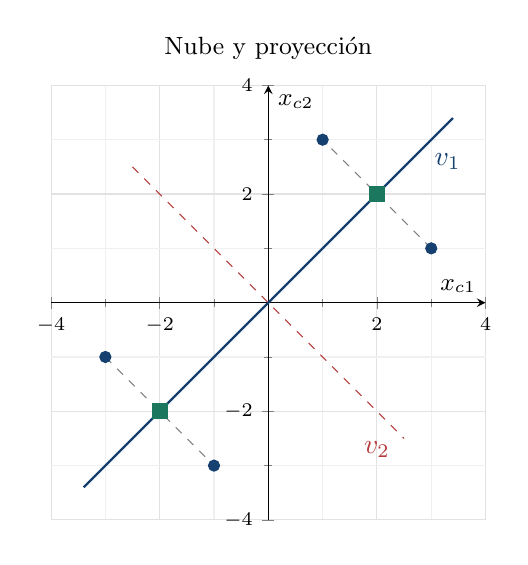
\begin{tikzpicture}
\begin{axis}[base,width=7.6cm,height=7.1cm,axis equal image,xmin=-4,xmax=4,ymin=-4,ymax=4,xlabel={$x_{c1}$},ylabel={$x_{c2}$},title={Nube y proyección},title style={font=\small}]
\addplot[azul,thick,domain=-3.4:3.4]{x};
\addplot[rojo,dashed,domain=-2.5:2.5]{-x};
\addplot[only marks,mark=*,mark size=2pt,azul]coordinates{(2,2)(3,1)(1,3)(-2,-2)(-3,-1)(-1,-3)};
\addplot[only marks,mark=square*,mark size=2.7pt,verde]coordinates{(2,2)(-2,-2)};
\draw[gray,dashed](axis cs:3,1)--(axis cs:2,2)--(axis cs:1,3);
\draw[gray,dashed](axis cs:-3,-1)--(axis cs:-2,-2)--(axis cs:-1,-3);
\node[azul]at(axis cs:3.3,2.6){$v_1$};\node[rojo]at(axis cs:2,-2.7){$v_2$};
\end{axis}
\end{tikzpicture}\hfill
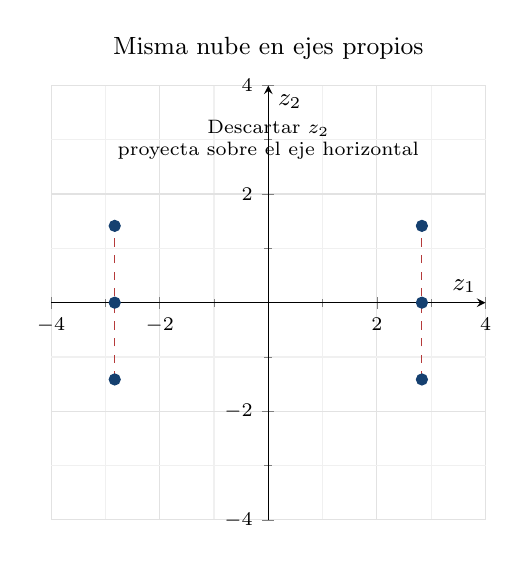
\begin{tikzpicture}
\begin{axis}[base,width=7.6cm,height=7.1cm,axis equal image,xmin=-4,xmax=4,ymin=-4,ymax=4,xlabel={$z_1$},ylabel={$z_2$},title={Misma nube en ejes propios},title style={font=\small}]
\addplot[only marks,mark=*,mark size=2pt,azul]coordinates{(2.828,0)(2.828,1.414)(2.828,-1.414)(-2.828,0)(-2.828,-1.414)(-2.828,1.414)};
\draw[rojo,dashed](axis cs:2.828,-1.414)--(axis cs:2.828,1.414);
\draw[rojo,dashed](axis cs:-2.828,-1.414)--(axis cs:-2.828,1.414);
\node[font=\scriptsize,align=center]at(axis cs:0,3){Descartar $z_2$\\proyecta sobre el eje horizontal};
\end{axis}
\end{tikzpicture}
\caption{Antes de descartar una coordenada, el cambio de base conserva las distancias. Los residuos aparecen verticales en el sistema de componentes.}
\end{figure}

\section{Geometría de elipses: covarianza y precisión}
Si $\Sigma\succ0$ y $\xi\sim N_p(\mu,\Sigma)$, su densidad es proporcional a
\[
\exp\left[-\frac12(x-\mu)\T\Sigma^{-1}(x-\mu)\right],\qquad x,\mu\in\R^{p\times1}.
\]
Con $\Sigma=V\Lambda V\T$ y $z=V\T(x-\mu)\in\R^{p\times1}$, los contornos satisfacen
\[
(x-\mu)\T\Sigma^{-1}(x-\mu)=\sum_{j=1}^p\frac{z_j^2}{\lambda_j}=c.
\]
Los semiejes tienen longitud $\sqrt{c\lambda_j}$. El autovalor mayor corresponde al eje largo de la elipse de covarianza. En cambio, para $x\T\Sigma x=c$, los semiejes son $\sqrt{c/\lambda_j}$: la relación se invierte.
\begin{ejemplo}[Una elipse rotada completamente calculada]
Para $\Sigma=\begin{psmallmatrix}3&1\\1&3\end{psmallmatrix}$, los autovalores son $4$ y $2$ y
\[
\Sigma^{-1}=\frac18\begin{pmatrix}3&-1\\-1&3\end{pmatrix},\qquad
\frac{3x_1^2-2x_1x_2+3x_2^2}{8}=1.
\]
Al definir $z_1=(x_1+x_2)/\sqrt2$ y $z_2=(x_1-x_2)/\sqrt2$, queda $z_1^2/4+z_2^2/2=1$. La elipse tiene semiejes $2$ y $\sqrt2$, rotados $45^\circ$ respecto a las variables originales.
\end{ejemplo}
\begin{figure}[H]\centering
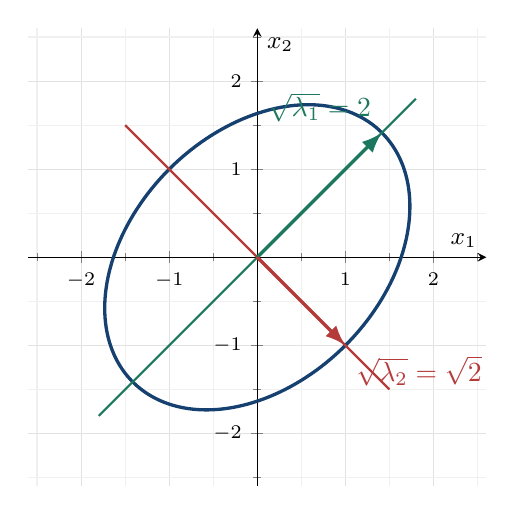
\begin{tikzpicture}
\begin{axis}[base,width=10.5cm,height=7.4cm,axis equal image,xmin=-2.6,xmax=2.6,ymin=-2.6,ymax=2.6,xlabel={$x_1$},ylabel={$x_2$}]
\addplot[azul,very thick,domain=0:360,samples=180]({sqrt(2)*cos(x)+sin(x)},{sqrt(2)*cos(x)-sin(x)});
\addplot[verde,thick,domain=-1.8:1.8]{x};\addplot[rojo,thick,domain=-1.5:1.5]{-x};
\draw[vecverde](axis cs:0,0)--(axis cs:1.4142,1.4142)node[above left]{$\sqrt{\lambda_1}=2$};
\draw[vecrojo](axis cs:0,0)--(axis cs:1,-1)node[below right]{$\sqrt{\lambda_2}=\sqrt2$};
\end{axis}\end{tikzpicture}
\caption{Contorno $x\T\Sigma^{-1}x=1$. Los autovectores fijan direcciones; las raíces de los autovalores fijan longitudes.}
\end{figure}
\subsection{Una figura no normal puede tener los mismos ejes de PCA}
PCA solo necesita segundos momentos. Muchas distribuciones diferentes comparten $\Sigma$ y, por tanto, los mismos ejes y autovalores. La elipse de covarianza describe dispersión cuadrática, pero no prueba normalidad ni determina por sí sola la forma completa de la nube.

\section{Ejemplo de tres variables: de un volumen a un plano}
Considérese la covarianza
\[
\Sigma=\frac16\begin{pmatrix}31&7&16\\7&31&16\\16&16&22\end{pmatrix}\in\R^{3\times3},\quad
v_1=\frac{(1,1,1)\T}{\sqrt3},\quad
v_2=\frac{(1,-1,0)\T}{\sqrt2},\quad
v_3=\frac{(1,1,-2)\T}{\sqrt6}.
\]
Todos los $v_j$ tienen dimensión $3\times1$; sus productos internos cruzados valen cero. Multiplicamos explícitamente:
\[
\Sigma(1,1,1)\T=\frac16(54,54,54)\T=9(1,1,1)\T,
\]
\[
\Sigma(1,-1,0)\T=\frac16(24,-24,0)\T=4(1,-1,0)\T,
\quad \Sigma(1,1,-2)\T=\frac16(6,6,-12)\T=(1,1,-2)\T.
\]
Por tanto, $\Lambda=\diag(9,4,1)$ y $\tr\Sigma=14$. Retener $k=2$ conserva $13/14\approx92.857\%$; retener solo uno conserva $9/14\approx64.286\%$.
\subsection{Proyección concreta y error exacto}
Para $x=(3,1,2)\T\in\R^{3\times1}$, suponiendo media cero,
\[
z_1=v_1\T x=2\sqrt3,\quad z_2=v_2\T x=\sqrt2,\quad z_3=v_3\T x=0.
\]
Este punto ya pertenece al plano principal. Para $y=(3,1,0)\T\in\R^{3\times1}$,
\[
a_1=\frac4{\sqrt3},\quad a_2=\sqrt2,\quad a_3=\frac4{\sqrt6},\qquad
\widehat y=a_1v_1+a_2v_2=(7/3,1/3,4/3)\T,
\]
\[
e=y-\widehat y=(2/3,2/3,-4/3)\T=a_3v_3,\quad
\norm e_2^2=\frac83,\quad v_1\T e=v_2\T e=0.
\]
El plano es $v_3\T y=0$, es decir, $y_1+y_2-2y_3=0$. Su proyector se obtiene sin resolver un nuevo sistema:
\[
P_2=I_3-v_3v_3\T=\frac16\begin{pmatrix}5&-1&2\\-1&5&2\\2&2&2\end{pmatrix},\qquad P_2y=\widehat y.
\]
\begin{figure}[H]\centering
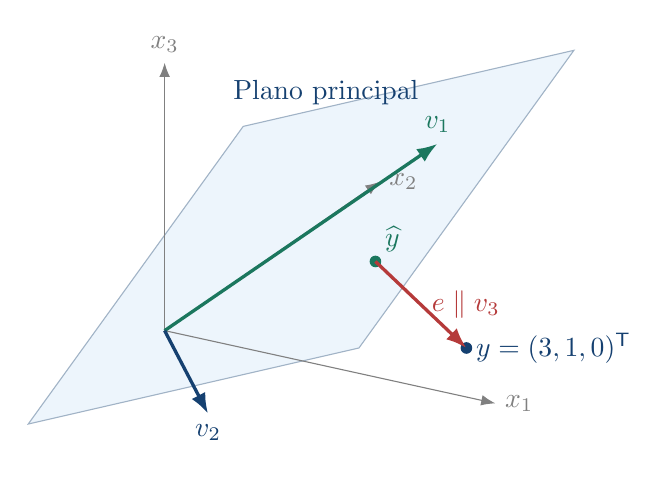
\begin{tikzpicture}[x={(1.0cm,-.22cm)},y={(.65cm,.45cm)},z={(0cm,.9cm)},scale=1.05]
\fill[celeste,opacity=.9](-1,-1,-1)--(3,-1,1)--(3,3,3)--(-1,3,1)--cycle;
\draw[azul!40](-1,-1,-1)--(3,-1,1)--(3,3,3)--(-1,3,1)--cycle;
\draw[eje](0,0,0)--(4,0,0)node[right]{$x_1$};\draw[eje](0,0,0)--(0,4,0)node[right]{$x_2$};\draw[eje](0,0,0)--(0,0,3.6)node[above]{$x_3$};
\draw[vecverde](0,0,0)--(2,2,2)node[above]{$v_1$};
\draw[vec](0,0,0)--(1.5,-1.5,0)node[below]{$v_2$};
\fill[azul](3,1,0)circle(2pt)node[right]{$y=(3,1,0)\T$};
\fill[verde](2.333,.333,1.333)circle(2pt)node[above right]{$\widehat y$};
\draw[vecrojo](2.333,.333,1.333)--(3,1,0)node[midway,right]{$e\parallel v_3$};
\node[azul]at(0,3,1.7){Plano principal};
\end{tikzpicture}
\caption{Reducción de tres variables a dos puntuaciones: el residuo queda en la dirección propia descartada. La perspectiva del dibujo no conserva ángulos.}
\end{figure}

\parte{III. Escalas, interpretación y descomposición en valores singulares}
\section{Covarianza o correlación: la métrica cambia la respuesta}
Sea $D=\diag(s_1,\ldots,s_p)\in\R^{p\times p}$, donde $s_j=\sqrt{s_{jj}}>0$. Los datos estandarizados son
\[
X_s=X_cD^{-1}\in\R^{n\times p},\quad (X_s)_{ij}=\frac{x_{ij}-\bar x_j}{s_j},\qquad
R=\frac1{n-1}X_s\T X_s=D^{-1}SD^{-1}.
\]
$R$ es la matriz de correlaciones, $r_{jj}=1$ y $\tr R=p$. Aplicar PCA a $R$ da la misma importancia inicial a una desviación estándar en cada variable. Aplicarlo a $S$ da importancia a diferencias medidas en unidades originales.
\begin{ejemplo}[El cambio de unidades puede cambiar el eje dominante]
Si $S=\diag(100,1)$, PCA de covarianzas conserva primero $(1,0)\T$, explicando $100/101$. Pero la correlación es $R=I_2$: ambas direcciones explican lo mismo. Si la primera variable se mide en metros o centímetros, su varianza se multiplica por $10^4$ al cambiar de metros a centímetros. La información observacional no cambió; la distancia euclidiana sí.
\end{ejemplo}
\subsection{Direcciones en coordenadas estandarizadas y originales}
Sea $a\in\R^{p\times1}$ un autovector unitario de $R$ con $Ra=\lambda a$. Su puntuación es
\[
z=X_sa=X_cD^{-1}a=X_cb,\qquad b=D^{-1}a\in\R^{p\times1}.
\]
En general $b\T b\ne1$, pero $b\T D^2b=1$. Además,
\[
D^{-1}SD^{-1}a=\lambda a\quad\Longleftrightarrow\quad Sb=\lambda D^2b.
\]
Se trata de un problema de autovalores generalizados. La reconstrucción original, para $A_k\in\R^{p\times k}$ con columnas propias de $R$, es
\[
\widehat X=\ones_n\bar x\T+X_sA_kA_k\T D.
\]
Minimiza el error estandarizado $\norm{(X-\widehat X)D^{-1}}\F^2$, no necesariamente el error sin ponderar $\norm{X-\widehat X}\F^2$.
\begin{cuidado}[Columnas constantes y criterios de escala]
Si $s_j=0$, no se puede dividir por $s_j$; esa columna no aporta varianza y se retira o se trata explícitamente. Estandarizar no es siempre obligatorio: si todas las variables comparten unidad y sus varianzas diferentes son significativas, PCA de covarianzas puede ser el objetivo adecuado. La elección debe corresponder al error que interesa minimizar.
\end{cuidado}

\section{Interpretar ejes, cargas, puntuaciones y biplots}
Un eje $v_j=(v_{1j},\ldots,v_{pj})\T\in\R^{p\times1}$ define
\[
z_{ij}=v_{1j}(x_{i1}-\bar x_1)+\cdots+v_{pj}(x_{ip}-\bar x_p).
\]
Coeficientes del mismo signo recogen movimientos conjuntos; signos contrarios describen contrastes. Pero el signo global es arbitrario: sustituir $v_j$ por $-v_j$ cambia $z_j$ por $-z_j$ y deja $z_jv_j\T$ igual.
\subsection{Dos usos del término ``carga''}
Algunos textos llaman cargas a los coeficientes $v_{aj}$; otros a correlaciones o a $v_{aj}\sqrt{\lambda_j}$. Hay que especificar la definición. Para la variable $a$, con desviación $s_a>0$, y la puntuación $z_j=X_cv_j\in\R^{n\times1}$,
\[
\widehat{\Cov}(X_a,z_j)=e_a\T Sv_j=\lambda_jv_{aj},\qquad
\boxed{\widehat{\Corr}(X_a,z_j)=\frac{\sqrt{\lambda_j}\,v_{aj}}{s_a}}
\quad(\lambda_j>0),
\]
donde $e_a\in\R^{p\times1}$ es el vector canónico con uno en la posición $a$. Para datos estandarizados $s_a=1$, y la correlación vale $\sqrt{\lambda_j}v_{aj}$.
\subsection{Varianza de cada variable reconstruida}
La covarianza reconstruida es $S_k=V_k\Lambda_kV_k\T$, por lo que
\[
(S_k)_{aa}=\sum_{j=1}^k\lambda_jv_{aj}^2,\qquad
h_a^2=\frac{\sum_{j=1}^k\lambda_jv_{aj}^2}{s_a^2}
=\sum_{j=1}^k\widehat{\Corr}(X_a,z_j)^2\in[0,1].
\]
$h_a^2$ mide qué proporción de la varianza de la variable $a$ conserva la representación. Una proporción global alta puede ocultar una variable mal representada.
\begin{ejemplo}[Cargas en el ejemplo maestro]
Allí $s_1=s_2=\sqrt{28/5}$ y $v_{11}=v_{21}=1/\sqrt2$. Por tanto,
\[
\Corr(X_1,z_1)=\Corr(X_2,z_1)=\sqrt{\frac{48/5}{2(28/5)}}=\sqrt{\frac67}\approx0.92582.
\]
Para la segunda componente las correlaciones son $\sqrt{1/7}$ y $-\sqrt{1/7}$. En cada variable las correlaciones cuadradas suman $6/7+1/7=1$ si conservamos ambos ejes.
\end{ejemplo}
\subsection{Por qué las flechas de un biplot no tienen una escala universal}
Si $X_c\approx U_kD_kV_k\T$, para $0\le\alpha\le1$ podemos escribir
\[
G=U_kD_k^\alpha\in\R^{n\times k},\quad B=V_kD_k^{1-\alpha}\in\R^{p\times k},\qquad
GB\T=U_kD_kV_k\T.
\]
Las filas de $G$ representan observaciones; las filas de $B$, variables. Su producto interno aproxima cada dato centrado. Distintas $\alpha$ cambian longitudes y la interpretación geométrica; solo en escalas adecuadas y con buena representación los ángulos entre flechas aproximan correlaciones.

\section{SVD: existencia, construcción y significado geométrico}
\begin{teorema}[Descomposición en valores singulares compacta]
Toda matriz $X_c\in\R^{n\times p}$ de rango $r$ admite
\[
\boxed{X_c=U_rD_rV_r\T=\sum_{j=1}^rd_j u_jv_j\T},\qquad
U_r\in\R^{n\times r},\ D_r\in\R^{r\times r},\ V_r\in\R^{p\times r},
\]
con $U_r\T U_r=V_r\T V_r=I_r$, $D_r=\diag(d_1,\ldots,d_r)$ y $d_1\ge\cdots\ge d_r>0$. Cada $u_j\in\R^{n\times1}$ y $v_j\in\R^{p\times1}$.
\end{teorema}
\begin{deduccion}
$X_c\T X_c$ es simétrica semidefinida positiva. El teorema espectral da autovectores $v_j$ y autovalores positivos $d_j^2$, $j\le r$. Define $u_j=X_cv_j/d_j$. Entonces
\[
u_i\T u_j=\frac{v_i\T X_c\T X_cv_j}{d_id_j}
=\frac{d_j^2v_i\T v_j}{d_id_j}=\delta_{ij}.
\]
Para $j>r$, $v_j\T X_c\T X_cv_j=\norm{X_cv_j}_2^2=0$, luego $X_cv_j=0$. Al expandir cualquier $x\in\R^{p\times1}$ en la base $\{v_j\}$,
\[
X_cx=\sum_{j=1}^r(v_j\T x)X_cv_j
=\sum_{j=1}^rd_j u_jv_j\T x.
\]
La igualdad para todo $x$ prueba la descomposición matricial.
\end{deduccion}
\subsection{Dos sistemas de coordenadas diferentes}
\[
X_cv_j=d_ju_j,\qquad X_c\T u_j=d_jv_j,\qquad
X_c\T X_cv_j=d_j^2v_j,\qquad X_cX_c\T u_j=d_j^2u_j.
\]
$V_r$ vive en el espacio de variables, dimensión $p$; $U_r$ vive en el espacio de observaciones, dimensión $n$. $X_c$ puede ser rectangular y por eso no tiene sentido general pedirle una ecuación $X_cv=\lambda v$: los dos lados tendrían dimensiones distintas.
\subsection{SVD completa y formas reducidas}
La SVD completa utiliza $U\in\R^{n\times n}$, $V\in\R^{p\times p}$ y una matriz diagonal rectangular $D\in\R^{n\times p}$. La SVD económica suele conservar $\min(n,p)$ columnas, algunas asociadas a ceros; la compacta conserva solo las $r$ positivas. No son convenciones idénticas.
\subsection{El puente exacto con PCA}
\[
S=\frac1{n-1}V_rD_r^2V_r\T,\qquad
\boxed{\lambda_j=\frac{d_j^2}{n-1}},\quad
\boxed{Z_r=X_cV_r=U_rD_r},\quad
\boxed{\widehat X_c=U_kD_kV_k\T}.
\]
Los valores singulares no son las varianzas; sus cuadrados, divididos por $n-1$, sí. Los vectores de $U_r$ no son puntuaciones con su escala original; hay que multiplicarlos por $D_r$.
\begin{idea}[Una descomposición, dos interpretaciones]
En álgebra, $X_c$ transforma direcciones $v_j$ en direcciones $u_j$, escaladas por $d_j$. En estadística, $v_j$ define una combinación de variables y $d_ju_j$ contiene sus puntuaciones en las $n$ observaciones.
\end{idea}

\section{SVD exacta del ejemplo maestro y la versión dual}
En la sección \ref{sec:ejemplo2d}, $n=6$, $p=r=2$:
\[
D_2=\begin{pmatrix}4\sqrt3&0\\0&2\sqrt2\end{pmatrix},\quad
u_1=\frac1{\sqrt6}(1,1,1,-1,-1,-1)\T\in\R^{6\times1},
\]
\[
u_2=\frac12(0,1,-1,0,-1,1)\T\in\R^{6\times1},\quad
U_2=[u_1\ u_2]\in\R^{6\times2},\quad
V_2=\frac1{\sqrt2}\begin{pmatrix}1&1\\1&-1\end{pmatrix}.
\]
Comprobamos $u_1\T u_1=6/6=1$, $u_2\T u_2=4/4=1$ y $u_1\T u_2=0$. Luego
\[
X_c=4\sqrt3\,u_1v_1\T+2\sqrt2\,u_2v_2\T,\quad
Z_1=4\sqrt3\,u_1,\quad \widehat X_c=4\sqrt3\,u_1v_1\T.
\]
La segunda pieza es exactamente la matriz residual calculada antes. Los valores singulares positivos son $d_1\approx6.928203$ y $d_2\approx2.828427$; sus cuadrados son $48$ y $8$.
\subsection{Cuando hay muchas más variables que observaciones}
Si $p\gg n$, formar una covarianza $p\times p$ puede ser caro. Podemos diagonalizar
\[
G=\frac1{n-1}X_cX_c\T\in\R^{n\times n},\qquad Gu_j=\lambda_ju_j.
\]
Para $\lambda_j>0$,
\[
v_j=\frac{X_c\T u_j}{\sqrt{(n-1)\lambda_j}}\in\R^{p\times1},\qquad
\norm{v_j}_2^2=\frac{u_j\T X_cX_c\T u_j}{(n-1)\lambda_j}=1,
\]
\[
Sv_j=\frac{X_c\T X_cX_c\T u_j}{(n-1)\sqrt{(n-1)\lambda_j}}=\lambda_jv_j.
\]
Esto recupera las mismas direcciones. No se divide por $\lambda_j=0$. En cómputo numérico, una SVD directa o truncada suele ser preferible a construir productos de Gram cuando preocupan precisión y condicionamiento.

\section{Eckart--Young--Mirsky: la mejor aproximación de rango bajo}
\begin{teorema}[Optimalidad en Frobenius y norma espectral]
Sea $X_c=\sum_{j=1}^rd_ju_jv_j\T$ y $1\le k<r$. Entre todas las matrices $B\in\R^{n\times p}$ con $\rank B\le k$, la truncación $X_{c,k}=\sum_{j=1}^kd_ju_jv_j\T$ satisface
\[
\min_{\rank B\le k}\norm{X_c-B}\F^2=\sum_{j=k+1}^rd_j^2,\qquad
\min_{\rank B\le k}\norm{X_c-B}_2=d_{k+1},
\]
donde $\norm A_2=\max_{\norm x_2=1}\norm{Ax}_2$ es la norma matricial espectral.
\end{teorema}
\begin{deduccion}
\textbf{Frobenius.} Sea $P$ el proyector ortogonal sobre el espacio de filas de $B$, de rango $q\le k$. Entonces $B=BP$ y
\[
X_c-B=X_c(I_p-P)+(X_cP-B).
\]
Ambos sumandos son ortogonales para el producto de Frobenius porque sus filas pertenecen a subespacios ortogonales. Por tanto,
\[
\norm{X_c-B}\F^2=\norm{X_c(I_p-P)}\F^2+\norm{X_cP-B}\F^2
\ge\norm{X_c}\F^2-\tr(PX_c\T X_c).
\]
El principio de máxima traza implica $\tr(PX_c\T X_c)\le\sum_{j=1}^q d_j^2\le\sum_{j=1}^kd_j^2$. Esto da la cota inferior. La truncación la alcanza porque sus términos residuales $d_ju_jv_j\T$ son ortogonales y tienen norma de Frobenius $d_j$.

\textbf{Espectral.} El subespacio $M=\spanop\{v_1,\ldots,v_{k+1}\}$ tiene dimensión $k+1$, mientras que $B$ tiene rango a lo sumo $k$. Existe $a\in M\cap\kerop B$, $\norm a_2=1$. Entonces
\[
\norm{X_c-B}_2\ge\norm{(X_c-B)a}_2=\norm{X_ca}_2
=\left(\sum_{j=1}^{k+1}d_j^2(v_j\T a)^2\right)^{1/2}\ge d_{k+1}.
\]
Para la truncación, el mayor valor singular del residuo es precisamente $d_{k+1}$, así que alcanza la cota.
\end{deduccion}
\subsection{Unicidad y degeneración}
Si $d_k>d_{k+1}$, la aproximación de rango $k$ óptima en Frobenius es única. Si el corte atraviesa un grupo de valores singulares iguales, distintas elecciones dentro de ese subespacio pueden producir diferentes aproximaciones con el mismo error. La unicidad en norma espectral es una cuestión distinta: no se deduce de la misma condición sin más.
\subsection{Compresión de una matriz y de una imagen}
Guardar $X_c$ requiere $np$ números. Una representación factorizada de rango $k$ utiliza aproximadamente $nk+pk+k$, además de la media si corresponde. Por ejemplo, para $n=1000$, $p=500$, $k=10$, son $15010$ números frente a $500000$. La reducción real de almacenamiento depende de precisión, formato y metadatos. Para una imagen matricial, la SVD aproxima intensidades; no exige interpretar filas como observaciones estadísticas.

\section{Varianza explicada, elección de dimensión y distancias}
Para $\tr S>0$, definimos
\[
\rho_j=\frac{\lambda_j}{\sum_{\ell=1}^p\lambda_\ell},\qquad
C_k=\sum_{j=1}^k\rho_j,\qquad
1-C_k=\frac{\norm{X_c-X_{c,k}}\F^2}{\norm{X_c}\F^2}.
\]
Una regla descriptiva es elegir el menor $k$ con $C_k\ge\tau$, por ejemplo $\tau=0.95$. El umbral es una decisión sobre error relativo de reconstrucción; no una ley estadística ni garantía predictiva.
\begin{ejemplo}[Un espectro que permite comparar criterios]
Sean los autovalores $(9,4,1,0.5,0.3,0.2)$, de suma $15$. Entonces
\[
(C_1,C_2,C_3,C_4,C_5,C_6)=(0.6,0.866667,0.933333,0.966667,0.986667,1).
\]
El $90\%$ exige tres componentes; el $95\%$, cuatro. El codo visual podría sugerir dos, pero eso responde a otro criterio y deja $13.333\%$ de varianza fuera.
\end{ejemplo}
\begin{figure}[H]\centering
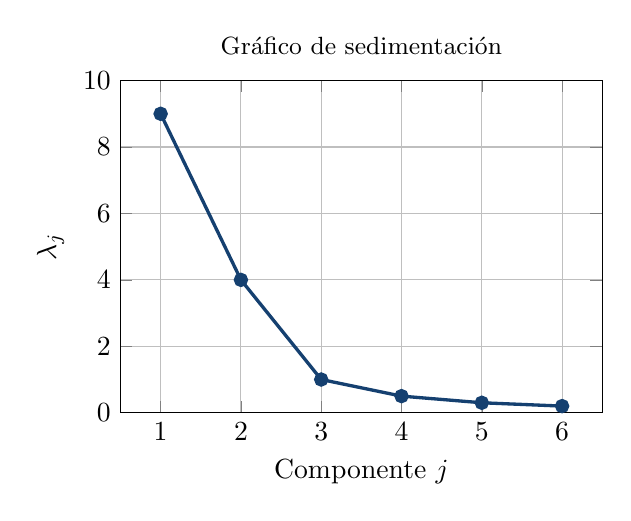
\begin{tikzpicture}
\begin{axis}[width=7.7cm,height=5.8cm,xlabel={Componente $j$},ylabel={$\lambda_j$},xtick={1,2,3,4,5,6},ymin=0,ymax=10,grid=major,title={Gráfico de sedimentación},title style={font=\small}]
\addplot[azul,very thick,mark=*]coordinates{(1,9)(2,4)(3,1)(4,.5)(5,.3)(6,.2)};
\end{axis}\end{tikzpicture}\hfill
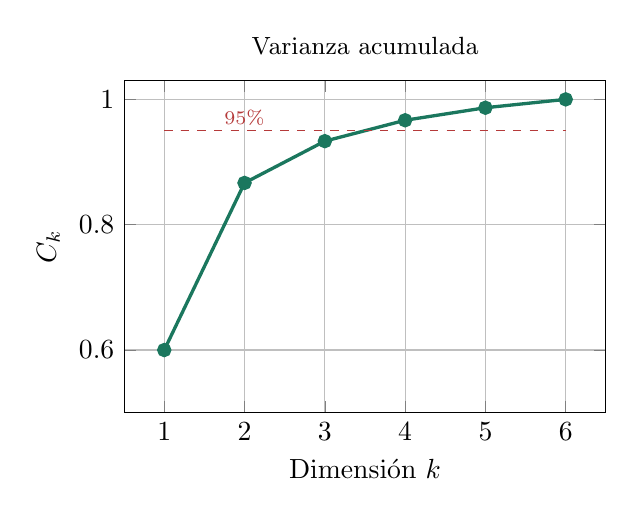
\begin{tikzpicture}
\begin{axis}[width=7.7cm,height=5.8cm,xlabel={Dimensión $k$},ylabel={$C_k$},xtick={1,2,3,4,5,6},ymin=.5,ymax=1.03,grid=major,title={Varianza acumulada},title style={font=\small}]
\addplot[verde,very thick,mark=*]coordinates{(1,.6)(2,.866667)(3,.933333)(4,.966667)(5,.986667)(6,1)};
\addplot[rojo,dashed,domain=1:6]{.95};\node[rojo,font=\scriptsize]at(axis cs:2,.97){$95\%$};
\end{axis}\end{tikzpicture}
\caption{Codo y umbral de varianza son herramientas distintas. La selección para predicción debe evaluar además el resultado supervisado.}
\end{figure}
\subsection{Criterios adicionales y sus límites}
El análisis paralelo compara autovalores observados con los de datos de referencia simulados bajo un modelo sin estructura común; depende de cómo se defina esa referencia. La validación de reconstrucción debe evaluar observaciones o entradas no usadas para ajustar; si solo se proyectan observaciones nuevas completas y se permite aumentar $k$ sin coste, el error disminuye al conservar más dimensiones. Para seleccionar un $k$ parsimonioso se necesita penalización, un objetivo de ruido o validación de entradas ocultas. En tareas supervisadas se elige $k$ dentro de la validación del predictor.
\subsection{PCA no conserva cada distancia con el mismo porcentaje}
Para dos observaciones $x_i,x_\ell\in\R^{p\times1}$, define $d=x_i-x_\ell$. Entonces
\[
\norm d_2^2=\norm{V_k\T d}_2^2+\norm{(I_p-P_k)d}_2^2,
\quad 0\le\norm{V_k\T d}_2^2\le\norm d_2^2.
\]
Cada distancia solo disminuye, pero puede colapsar totalmente si $d$ está en el espacio descartado. Sí hay una identidad global:
\[
\sum_{i<\ell}\norm{x_i-x_\ell}_2^2=n\sum_i\norm{x_i-\bar x}_2^2=n\norm{X_c}\F^2.
\]
\textbf{Demostración.} La suma sobre todos los pares ordenados es $2n\sum_i\norm{x_i}_2^2-2\norm{\sum_ix_i}_2^2$; dividir por dos y centrar da el resultado. Aplicando la identidad a los residuos, PCA minimiza la \emph{suma} de pérdidas de distancias cuadradas entre pares para proyecciones ortogonales de dimensión $k$; no la peor distorsión relativa.

\section{Blanqueamiento, Mahalanobis y la geometría de identidad}
Supón $S\succ0$ y $S=V\Lambda V\T$. Los datos de PCA rotados $Z=X_cV$ tienen covarianza $\Lambda$, que es diagonal pero no suele ser identidad. Para hacerla identidad se escala:
\[
W_{\mathrm{PCA}}=X_cV\Lambda^{-1/2}\in\R^{n\times p},\qquad
\frac1{n-1}W_{\mathrm{PCA}}\T W_{\mathrm{PCA}}=I_p.
\]
Este es el blanqueamiento PCA. El blanqueamiento simétrico o ZCA es
\[
W_{\mathrm{ZCA}}=X_cS^{-1/2}=X_cV\Lambda^{-1/2}V\T\in\R^{n\times p}.
\]
También tiene covarianza identidad, pero vuelve a las coordenadas originales mediante $V\T$.
\subsection{Mahalanobis se vuelve Euclides}
Para $x,y\in\R^{p\times1}$,
\[
d_M(x,y)^2=(x-y)\T S^{-1}(x-y)
=\norm{\Lambda^{-1/2}V\T(x-y)}_2^2.
\]
Una diferencia grande en una dirección muy variable cuenta menos; una diferencia pequeña en una dirección de varianza minúscula puede contar mucho. Esto explica por qué blanquear puede amplificar ruido si hay autovalores muy pequeños.
\begin{ejemplo}[La identidad aparece por una transformación, no por casualidad]
Para $S=\begin{psmallmatrix}3&1\\1&3\end{psmallmatrix}$, $\Lambda=\diag(4,2)$. Si $z=(z_1,z_2)\T$ son coordenadas principales,
\[
w=(z_1/2,z_2/\sqrt2)\T\in\R^{2\times1},\qquad\Cov(w)=I_2.
\]
PCA solo dio covarianza $\diag(4,2)$; dividir por las desviaciones $2$ y $\sqrt2$ es el paso adicional.
\end{ejemplo}
\subsection{Singularidad, pseudoinversa y regularización}
Si solo hay $r<p$ autovalores positivos, $S^{-1}$ no existe. La pseudoinversa es
\[
S^+=V_r\Lambda_r^{-1}V_r\T\in\R^{p\times p}.
\]
Se puede blanquear a $r$ dimensiones mediante $X_cV_r\Lambda_r^{-1/2}$, cuya covarianza es $I_r$. En $p$ dimensiones, $S^{+1/2}SS^{+1/2}=V_rV_r\T$, un proyector, no $I_p$. Usar $(S+\alpha I_p)^{-1/2}$ con $\alpha>0$ evita divisiones extremas, pero la covarianza transformada tiene autovalores $\lambda_j/(\lambda_j+\alpha)$, no exactamente uno.

\parte{IV. Aprendizaje automático y econometría: qué aporta PCA}
\section{PCA frente a regresión: proyecciones en espacios distintos}
Para regresión lineal centrada, $y_c\in\R^{n\times1}$ es una respuesta y $X_c\in\R^{n\times p}$ contiene predictores. MCO busca
\[
\min_{\beta\in\R^{p\times1}}\norm{y_c-X_c\beta}_2^2,
\qquad X_c\T X_c\widehat\beta=X_c\T y_c.
\]
Si $X_c$ tiene rango columna completo, $\widehat\beta=(X_c\T X_c)^{-1}X_c\T y_c$. En cambio, PCA no recibe $y_c$ y busca aproximar $X_c$ mismo.
\subsection{Dos operadores de proyección que no deben confundirse}
Con la SVD compacta $X_c=U_rD_rV_r\T$,
\[
P_{\mathrm{obs}}=U_rU_r\T\in\R^{n\times n},\qquad
P_{\mathrm{var}}=V_kV_k\T\in\R^{p\times p}.
\]
MCO proyecta $y_c$ en el espacio columna de $X_c$: $\widehat y_c=P_{\mathrm{obs}}y_c$. PCA proyecta las \emph{filas} de $X_c$ en un subespacio del espacio de variables: $\widehat X_c=X_cP_{\mathrm{var}}$. Las dimensiones revelan la diferencia.
\subsection{Regresión vertical frente a distancia perpendicular}
Si una nube bidimensional tiene covarianza $S=\begin{psmallmatrix}a&b\\b&c\end{psmallmatrix}$, con $a>0$, la pendiente de la regresión de la segunda variable sobre la primera es $b/a$. La pendiente de la primera componente, cuando $v_{11}\ne0$, es $v_{21}/v_{11}$, obtenida por el autovector dominante. Para el ejemplo maestro,
\[
\text{pendiente MCO}=\frac{4}{28/5}=\frac57,\qquad
\text{pendiente PCA}=1.
\]
MCO minimiza errores verticales en una variable designada como respuesta; PCA minimiza distancias perpendiculares tratando ambas variables simétricamente dentro de la métrica elegida.
\begin{figure}[H]\centering
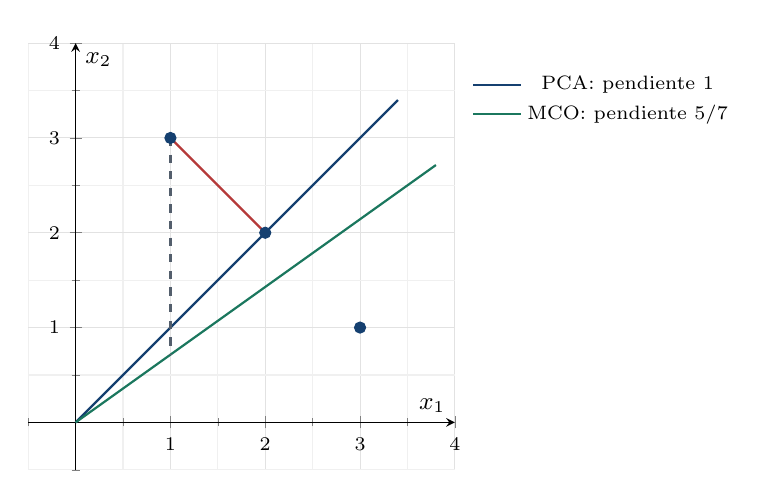
\begin{tikzpicture}
\begin{axis}[base,width=10cm,height=7cm,axis equal image,xmin=-.5,xmax=4,ymin=-.5,ymax=4,xlabel={$x_1$},ylabel={$x_2$},legend style={at={(1.02,.95)},anchor=north west}]
\addplot[azul,thick,domain=0:3.4]{x};\addlegendentry{PCA: pendiente 1}
\addplot[verde,thick,domain=0:3.8]{5*x/7};\addlegendentry{MCO: pendiente $5/7$}
\addplot[only marks,mark=*,azul]coordinates{(1,3)(2,2)(3,1)};
\draw[rojo,thick](axis cs:1,3)--(axis cs:2,2);
\draw[gris,dashed,thick](axis cs:1,3)--(axis cs:1,.714286);
\end{axis}\end{tikzpicture}
\caption{Se muestran los tres puntos positivos del ejemplo maestro. El segmento rojo es perpendicular a la recta PCA; el gris mide el error vertical para MCO.}
\end{figure}

\section{Regresión por componentes principales: deducción y sesgo}
En PCR se conserva $Z_k=X_cV_k=U_kD_k\in\R^{n\times k}$ y se ajusta
\[
y_c=Z_k\gamma+\varepsilon,\qquad \gamma\in\R^{k\times1},\quad\varepsilon\in\R^{n\times1}.
\]
Como $Z_k\T Z_k=D_k^2$,
\[
\widehat\gamma=(Z_k\T Z_k)^{-1}Z_k\T y_c=D_k^{-1}U_k\T y_c,
\]
\[
\boxed{\widehat\beta_{\mathrm{PCR},k}=V_kD_k^{-1}U_k\T y_c\in\R^{p\times1}},\qquad
\widehat y_c=U_kU_k\T y_c.
\]
El intercepto recuperado es $\widehat\beta_0=\bar y-\bar x\T\widehat\beta_{\mathrm{PCR},k}$. Usar todas las componentes de rango positivo produce la solución MCO de mínima norma, incluso si $p>n$.
\subsection{Descomposición de sesgo y varianza condicional}
Supón $y_c=X_c\beta+\varepsilon$ en el espacio centrado, con ruido original homocedástico de varianza $\sigma^2$; en las direcciones de $U_r$, su covarianza sigue siendo $\sigma^2I_r$. Fijado $X_c$,
\[
\E[\widehat\beta_{\mathrm{PCR},k}\mid X_c]=V_kV_k\T\beta,\qquad
\Cov(\widehat\beta_{\mathrm{PCR},k}\mid X_c)=\sigma^2V_kD_k^{-2}V_k\T.
\]
Escribe $\beta=\sum_{j=1}^p b_jv_j$, con $b_j=v_j\T\beta$. Entonces
\[
\E[\norm{\widehat\beta_{\mathrm{PCR},k}-\beta}_2^2\mid X_c]
=\sum_{j=k+1}^pb_j^2+\sigma^2\sum_{j=1}^k\frac1{d_j^2}.
\]
Se reduce varianza al evitar dividir por valores singulares pequeños, pero se introduce sesgo si $\beta$ tiene componentes en ejes descartados. Para predecir en el diseño observado,
\[
\E[\norm{X_c\widehat\beta_{\mathrm{PCR},k}-X_c\beta}_2^2\mid X_c]
=\sum_{j=k+1}^rd_j^2b_j^2+\sigma^2k.
\]
Estas expresiones separan error de estimación de coeficientes y error de predicción; no son intercambiables.
\begin{ejemplo}[Una señal importante puede tener varianza pequeña]
Sean variables independientes $\xi_1\sim N(0,100)$ y $\xi_2\sim N(0,0.01)$, con respuesta $Y=10\xi_2$. PCA conserva primero $\xi_1$, que explica $100/100.01\approx99.990\%$ de la varianza de predictores. Pero $Y$ depende solo de la segunda variable. Usando solo la primera, el mejor predictor cuadrático es $\E[Y\mid\xi_1]=0$ y su error es $\Var(Y)=1$. Conservando la segunda, la predicción es exacta. Mucha varianza explicada en $X$ no asegura buena predicción de $Y$.
\end{ejemplo}

\section{Ridge, pseudoinversa y filtros espectrales}
Ridge resuelve, para $\alpha>0$,
\[
\min_{\beta\in\R^{p\times1}}\norm{y_c-X_c\beta}_2^2+\alpha\norm\beta_2^2,
\qquad\widehat\beta_{\mathrm{ridge}}=(X_c\T X_c+\alpha I_p)^{-1}X_c\T y_c.
\]
Sustituyendo la SVD,
\[
\widehat\beta_{\mathrm{ridge}}=\sum_{j=1}^r\frac{d_j}{d_j^2+\alpha}v_ju_j\T y_c,
\qquad
\widehat y_c=\sum_{j=1}^r\frac{d_j^2}{d_j^2+\alpha}u_ju_j\T y_c.
\]
La pseudoinversa de $X_c$ es $X_c^+=V_rD_r^{-1}U_r\T\in\R^{p\times n}$, y la solución MCO de mínima norma es $X_c^+y_c$.
\begin{center}\small
\begin{tabular}{lll}\toprule
Método & Factor sobre $u_ju_j\T y_c$ & Acción\\\midrule
MCO de mínima norma & $1$ para $d_j>0$ & Conserva toda dirección identificable\\
PCR con $k$ & $\ind_{\{j\le k\}}$ & Corte abrupto de direcciones\\
Ridge & $d_j^2/(d_j^2+\alpha)$ & Atenuación continua\\\bottomrule
\end{tabular}\end{center}
\subsection{Ejemplo numérico de la atenuación}
Si $d_1^2=48$, $d_2^2=8$ y $\alpha=8$, los factores de predicción ridge son $48/56=6/7$ y $8/16=1/2$. PCR con $k=1$ usa $1$ y $0$. No son el mismo procedimiento: ambos controlan direcciones poco estables, pero hacen compromisos diferentes.
\subsection{El número efectivo de parámetros}
Para ridge, la matriz suavizadora es $H_\alpha=U_r\diag(d_j^2/(d_j^2+\alpha))U_r\T\in\R^{n\times n}$ y
\[
\operatorname{df}_{\mathrm{ridge}}=\tr(H_\alpha)=\sum_{j=1}^r\frac{d_j^2}{d_j^2+\alpha}.
\]
Para PCR con ejes y $k$ fijos, $\tr(U_kU_k\T)=k$. Si $k$ se selecciona utilizando la respuesta, la complejidad total de la selección no queda completamente descrita por ese $k$.

\section{PCA dentro de un flujo de aprendizaje automático}
\subsection{Entrenar, transformar y evaluar sin fuga de información}
El conjunto de entrenamiento determina $\bar x$, las escalas $D$, los ejes $V_k$ y cualquier elección de $k$. En validación se aplica
\[
z_{\mathrm{val}}=V_k\T D^{-1}(x_{\mathrm{val}}-\bar x)\in\R^{k\times1},
\]
con $D=I_p$ si no se estandariza. Ajustar PCA antes de separar validación utiliza la distribución de los datos que se pretende evaluar; puede contaminar la evaluación aunque PCA no use etiquetas. En validación cruzada se repite todo el ajuste dentro de cada partición.
\subsection{Clasificación, agrupamiento y detección de anomalías}
Un clasificador puede usar $z_i$ como entrada; por ejemplo, en una regresión logística,
\[
\Pr(Y_i=1\mid z_i)=\frac1{1+\exp[-(\beta_0+\gamma\T z_i)]},\qquad
\gamma\in\R^{k\times1}.
\]
En coordenadas originales, el coeficiente es $D^{-1}V_k\gamma\in\R^{p\times1}$. La restricción a ese subespacio puede mejorar estabilidad o eliminar señal predictiva; se decide con evaluación supervisada.

En agrupamiento, las distancias entre puntuaciones pueden eliminar ruido, pero también borrar grupos diferenciados en direcciones de baja varianza. Para anomalías conviene distinguir
\[
T_i^2=z_i\T\Lambda_k^{-1}z_i,\qquad
Q_i=\norm{(I_p-P_k)(x_i-\bar x)}_2^2.
\]
$T_i^2$ detecta puntuaciones extremas dentro del subespacio; $Q_i$ detecta desviaciones fuera de él. Sus umbrales estadísticos requieren un modelo y un esquema de estimación; no se toma automáticamente una distribución chi-cuadrado para ambos.
\subsection{Datos faltantes, valores atípicos y variables categóricas}
PCA ordinario requiere una matriz numérica completa. Imputar con medias puede reducir artificialmente varianza y covarianza. Una alternativa es ajustar rango bajo usando solo entradas observadas; otra es un modelo probabilístico. Los atípicos pueden dominar la covarianza porque las desviaciones se elevan al cuadrado. Las variables categóricas codificadas como enteros no adquieren una distancia cuantitativa válida por el mero hecho de tener números; puede ser necesario otro tipo de representación o análisis.
\begin{cuidado}[Interpretación y causalidad]
Una componente explica dispersión, no causas. Un eje con cargas altas en ingreso, educación y consumo puede resumir una asociación, pero no identifica un efecto causal ni una variable latente única. Su nombre es una interpretación sustantiva que debe contrastarse con el diseño y las variables.
\end{cuidado}

\section{Autoencoders lineales: por qué reaparece el subespacio PCA}
Un autoencoder lineal centrado usa un codificador $B\in\R^{p\times k}$ y un decodificador $C\in\R^{k\times p}$:
\[
Z=X_cB\in\R^{n\times k},\qquad\widehat X_c=X_cBC\in\R^{n\times p},\qquad
\min_{B,C}\norm{X_c-X_cBC}\F^2.
\]
Como $\rank(X_cBC)\le k$, el teorema de mejor aproximación impone un error al menos $\sum_{j>k}d_j^2$. Se alcanza con $B=V_k$ y $C=V_k\T$; por tanto el mínimo global coincide con PCA.
\subsection{El código latente no tiene que ser una componente principal}
Para cualquier matriz invertible $R\in\R^{k\times k}$,
\[
B=V_kR,\qquad C=R^{-1}V_k\T\quad\Rightarrow\quad BC=V_kV_k\T.
\]
La reconstrucción es la misma, pero el código $X_cV_kR$ puede tener coordenadas correlacionadas, escalas distintas y ejes no ortogonales. Coincidir en subespacio óptimo no implica recuperar individualmente los autovectores. Con no linealidades, regularización o pérdidas diferentes, el problema deja de ser PCA en general.
\subsection{Un cuello de botella no prueba una estructura causal}
Una representación que reconstruye bien puede mezclar factores interpretables de muchas maneras. Identificar factores o mecanismos necesita restricciones adicionales; el tamaño $k$ del código, por sí solo, no proporciona esa identificación.

\section{PCA probabilístico: variables latentes y ruido isotrópico}
En PPCA se postula, para cada observación aleatoria $\xi\in\R^{p\times1}$,
\[
\xi=\mu+Wh+\varepsilon,\quad
h\sim N_k(0,I_k),\quad\varepsilon\sim N_p(0,\sigma^2I_p),\quad h\perp\!\!\!\perp\varepsilon,
\]
con $W\in\R^{p\times k}$, $\mu\in\R^{p\times1}$ y $\sigma^2>0$. Integrando $h$,
\[
\xi\sim N_p(\mu,C),\qquad C=WW\T+\sigma^2I_p\in\R^{p\times p}.
\]
El ruido tiene la misma varianza en todas las direcciones; es una hipótesis fuerte, distinta de exigir simplemente segundos momentos.
\subsection{Verosimilitud y estimación de la media}
Para observaciones independientes, omitiendo constantes,
\[
\ell(\mu,W,\sigma^2)=-\frac n2\log\det C
-\frac12\sum_i(x_i-\mu)\T C^{-1}(x_i-\mu).
\]
Derivar respecto a $\mu$ da $C^{-1}\sum_i(x_i-\mu)=0$, así que $\widehat\mu=\bar x$. Con $S_n=X_c\T X_c/n$,
\[
\ell=-\frac n2\left[\log\det C+\tr(C^{-1}S_n)\right]+\text{constante}.
\]
Aquí los autovalores relevantes son $\ell_1\ge\cdots\ge\ell_p\ge0$ de $S_n$, no los de $S$; $\ell_j=(n-1)\lambda_j/n$.
\subsection{Solución espectral y origen de la varianza de ruido}
Para $k<p$, en el caso interior no degenerado,
\[
\widehat\sigma^2=\frac1{p-k}\sum_{j=k+1}^p\ell_j,\qquad
\widehat W=V_k(\operatorname{diag}(\ell_1,\ldots,\ell_k)-\widehat\sigma^2I_k)^{1/2}R,
\]
con $R\in\R^{k\times k}$ ortogonal. La solución exige $\ell_j\ge\widehat\sigma^2$ en los ejes retenidos; si hay igualdades, algunas cargas se anulan. Si el promedio residual es cero, el óptimo puede estar en la frontera $\sigma^2=0$, donde la densidad no degenerada requiere tratamiento límite.
\begin{deduccion}
Fijados los autovalores de $C$, el término $\log\det C$ no depende de sus ejes. La traza $\tr(C^{-1}S_n)$ se minimiza alineando mayores autovalores de $S_n$ con mayores autovalores de $C$: si dos pares están invertidos, el cambio de coste al intercambiarlos es
\[
\frac{\ell_a}{c_a}+\frac{\ell_b}{c_b}-\frac{\ell_a}{c_b}-\frac{\ell_b}{c_a}
=(\ell_a-\ell_b)(c_a^{-1}-c_b^{-1})\le0
\]
cuando $\ell_a\ge\ell_b$ y $c_a\ge c_b$. La extensión a bases ortogonales se obtiene porque los cuadrados de los productos entre ejes forman una matriz doblemente estocástica y la traza es lineal en esos pesos. El mínimo está en una alineación de ejes.

En los $k$ ejes de señal, $c_j=\sigma^2+\omega_j^2$; en los restantes, $c_j=\sigma^2$. El objetivo escalar es
\[
\sum_{j=1}^k\left(\log c_j+\frac{\ell_j}{c_j}\right)
+(p-k)\log\sigma^2+\frac{\sum_{j>k}\ell_j}{\sigma^2}.
\]
Derivar $\log c+\ell/c$ da $(c-\ell)/c^2$; el mínimo es $c_j=\ell_j$ para ejes activos. Derivar respecto a $s=\sigma^2$ en el bloque restante da $(p-k)/s-\sum_{j>k}\ell_j/s^2=0$, de donde el promedio residual. Finalmente $WW\T=V_k\diag(\ell_j-\widehat\sigma^2)V_k\T$ permite cualquier rotación latente $R$.
\end{deduccion}
\subsection{Distribución posterior del factor latente: completar cuadrados}
Define $M=W\T W+\sigma^2I_k\in\R^{k\times k}$ y $y=x-\mu\in\R^{p\times1}$. La densidad condicional de $h$ es proporcional a
\[
\exp\left[-\frac12h\T h-\frac1{2\sigma^2}(y-Wh)\T(y-Wh)\right].
\]
Al agrupar términos en $h$,
\[
h\T Mh-2h\T W\T y
=(h-M^{-1}W\T y)\T M(h-M^{-1}W\T y)-y\T WM^{-1}W\T y.
\]
Por tanto,
\[
\boxed{h\mid x\sim N_k(M^{-1}W\T(x-\mu),\ \sigma^2M^{-1})}.
\]
El código posterior encoge y escala las puntuaciones; no es simplemente $V_k\T(x-\mu)$. PPCA permite cuantificar incertidumbre latente y tratar datos incompletos dentro de un modelo. La formulación probabilística clásica se debe a Tipping y Bishop; su artículo se incluye en las referencias.
\subsection{PCA frente a análisis factorial}
En análisis factorial, $\Cov(\varepsilon)=\Psi$ suele ser diagonal con entradas diferentes; entonces $C=WW\T+\Psi$. Esto distingue variación específica por variable de variación común. PCA descompone varianza total sin ese modelo; PPCA es un modelo particular con $\Psi=\sigma^2I_p$. Las tres formulaciones no deben usarse como sinónimos.

\parte{V. Portafolios: la conexión precisa con autovectores y PCA}
\section{Retornos, pesos y varianza como forma cuadrática}
Sea $R=(R_1,\ldots,R_p)\T\in\R^{p\times1}$ un vector aleatorio de retornos, $\mu=\E[R]\in\R^{p\times1}$ y $\Sigma=\Cov(R)\in\R^{p\times p}$. Un vector de pesos $w=(w_1,\ldots,w_p)\T\in\R^{p\times1}$ produce
\[
R_P=w\T R=\sum_jw_jR_j,\quad
\mu_P=w\T\mu,\quad
\sigma_P^2=\Var(w\T R)=w\T\Sigma w.
\]
Con presupuesto total invertido, $\ones_p\T w=1$. Si se prohíben posiciones cortas, además $w_j\ge0$. Un peso negativo significa una posición corta dentro del modelo; no es un error algebraico, aunque puede estar excluido por la aplicación.
\subsection{Expansión para dos activos}
Con $w=(a,1-a)\T$, desviaciones $\sigma_1,\sigma_2$ y correlación $\rho$,
\[
\Sigma=\begin{pmatrix}\sigma_1^2&\rho\sigma_1\sigma_2\\\rho\sigma_1\sigma_2&\sigma_2^2\end{pmatrix},\quad
\sigma_P^2=a^2\sigma_1^2+(1-a)^2\sigma_2^2+2a(1-a)\rho\sigma_1\sigma_2.
\]
La diversificación procede del término de covarianza. No basta contar activos: si se mueven de manera casi idéntica, la reducción de riesgo puede ser limitada.
\begin{ejemplo}[Dos activos con riesgo y correlación distintos]
Tomemos datos hipotéticos, en una misma unidad temporal:
\[
\mu=(0.08,0.14)\T,\quad
\Sigma=\begin{pmatrix}0.04&0.006\\0.006&0.09\end{pmatrix},\quad
\sigma_1=0.20,\quad\sigma_2=0.30,\quad\rho=0.10.
\]
Para $w=(1/2,1/2)\T$,
\[
\mu_P=0.11,\qquad \sigma_P^2=0.25(0.04)+0.25(0.09)+0.5(0.006)=0.0355,
\quad\sigma_P\approx0.188414.
\]
La desviación del portafolio es menor que la de cualquiera de los dos activos en este ejemplo. Todos los valores son ilustrativos; no son cotizaciones ni estimaciones de una inversión real.
\end{ejemplo}

\section{Cuándo el portafolio sí lleva a una ecuación propia}
Consideremos primero un problema geométrico de exposición con \emph{norma} fija:
\[
\min_{w\T w=1}w\T\Sigma w\qquad\text{o}\qquad
\max_{w\T w=1}w\T\Sigma w.
\]
Su lagrangiano es $\mathcal L=w\T\Sigma w-\lambda(w\T w-1)$, por lo que
\[
2\Sigma w-2\lambda w=0\quad\Longleftrightarrow\quad
\boxed{\Sigma w=\lambda w}.
\]
El mínimo se alcanza en el autoespacio de $\lambda_p$ y el máximo en el de $\lambda_1$. El problema de PCA es el de \emph{máxima} varianza con esta normalización.
\subsection{La restricción determina el lado derecho}
Con presupuesto, el problema es $\min w\T\Sigma w$ sujeto a $\ones_p\T w=1$. Ahora
\[
\mathcal L=w\T\Sigma w-2\eta(\ones_p\T w-1),\qquad
2\Sigma w-2\eta\ones_p=0,
\]
\[
\boxed{\Sigma w=\eta\ones_p}.
\]
El lado derecho es el vector de unos, no $w$. Se parece a una ecuación propia porque ambas surgen de formas cuadráticas, pero la derivada de la restricción cambió.
\begin{center}\small
\begin{tabular}{p{4.2cm}p{5.2cm}p{5.6cm}}\toprule
Restricción & Condición de primer orden & Interpretación\\\midrule
$w\T w=1$ & $\Sigma w=\lambda w$ & Autovector ordinario; riesgo por norma\\
$\ones_p\T w=1$ & $\Sigma w=\eta\ones_p$ & Portafolio con presupuesto\\
$w\T Bw=1$, $B\succ0$ & $\Sigma w=\lambda Bw$ & Autovector generalizado\\
$\ones_p\T w=1$, $\mu\T w=m$ & $\Sigma w=\eta\ones_p+\gamma\mu$ & Riesgo mínimo para retorno fijado\\\bottomrule
\end{tabular}\end{center}
\begin{cuidado}[Normalizar un autovector no resuelve automáticamente Markowitz]
Si $v$ es un autovector y $\ones_p\T v\ne0$, podemos imponer presupuesto con $w=v/(\ones_p\T v)$. Eso vuelve factible el vector, pero no garantiza optimalidad de mínima varianza con presupuesto. Si $\ones_p\T v=0$, ni siquiera se puede hacer esa normalización: es una exposición de inversión neta cero.
\end{cuidado}

\section{Portafolio global de mínima varianza: solución y prueba}
Supongamos $\Sigma\succ0$ y pesos reales sin otras restricciones. De $\Sigma w=\eta\ones_p$,
\[
w=\eta\Sigma^{-1}\ones_p,\quad1=\ones_p\T w=\eta\ones_p\T\Sigma^{-1}\ones_p.
\]
Definiendo $a=\ones_p\T\Sigma^{-1}\ones_p>0$,
\[
\boxed{w_{\mathrm{GMV}}=\frac{\Sigma^{-1}\ones_p}{\ones_p\T\Sigma^{-1}\ones_p}},\qquad
\boxed{\sigma_{\mathrm{GMV}}^2=\frac1a}.
\]
\subsection{Demostración directa de que el mínimo es global y único}
Cualquier otro peso factible es $w=w_{\mathrm{GMV}}+h$, con $h\in\R^{p\times1}$ y $\ones_p\T h=0$. Entonces
\[
w\T\Sigma w=w_{\mathrm{GMV}}\T\Sigma w_{\mathrm{GMV}}+2h\T\Sigma w_{\mathrm{GMV}}+h\T\Sigma h
=\frac1a+\frac2a h\T\ones_p+h\T\Sigma h=\frac1a+h\T\Sigma h.
\]
La positividad estricta da $h\T\Sigma h>0$ para $h\ne0$. Esto verifica suficiencia y unicidad sin confiar únicamente en las derivadas.
\subsection{Ejemplo de dos activos: números completos}
Para la covarianza anterior,
\[
\det\Sigma=0.04(0.09)-0.006^2=0.003564,\qquad
\Sigma^{-1}=\frac1{0.003564}\begin{pmatrix}0.09&-0.006\\-0.006&0.04\end{pmatrix},
\]
\[
\Sigma^{-1}\ones_2=\frac1{0.003564}(0.084,0.034)\T,\quad
w_{\mathrm{GMV}}=\frac1{0.118}(0.084,0.034)\T
=\left(\frac{42}{59},\frac{17}{59}\right)\T.
\]
\[
\mu_{\mathrm{GMV}}=0.09728814,\qquad
\sigma_{\mathrm{GMV}}^2=\frac{0.003564}{0.118}=0.03020339,\quad
\sigma_{\mathrm{GMV}}\approx0.17379122.
\]
Comprobamos la condición vectorial:
\[
\Sigma w_{\mathrm{GMV}}
=\begin{pmatrix}0.04(42/59)+0.006(17/59)\\0.006(42/59)+0.09(17/59)\end{pmatrix}
=0.03020339\begin{pmatrix}1\\1\end{pmatrix}.
\]
El vector no es un autovector de $\Sigma$: sus componentes no son iguales y el lado derecho tiene componentes iguales.
\subsection{La misma fórmula derivada en una sola variable}
Para $w=(t,1-t)\T$ y $\Sigma=\begin{psmallmatrix}a_0&c_0\\c_0&b_0\end{psmallmatrix}$,
\[
f(t)=a_0t^2+b_0(1-t)^2+2c_0t(1-t),\quad
f'(t)=2(a_0+b_0-2c_0)t+2(c_0-b_0).
\]
Si $a_0+b_0-2c_0>0$, el mínimo sin restricciones de signo es
\[
t^*=\frac{b_0-c_0}{a_0+b_0-2c_0}.
\]
Con prohibición de cortos en dos activos, el mínimo es la proyección de $t^*$ sobre $[0,1]$. En más activos no basta recortar coordenadas y renormalizar: hay que resolver las condiciones de optimalidad conjunta.

\section{Frontera media--varianza: derivación matricial completa}
Fijado un retorno objetivo $m\in\R$, resolvemos
\[
\min_{w\in\R^{p\times1}}\frac12w\T\Sigma w
\quad\text{sujeto a }\ones_p\T w=1,\quad\mu\T w=m.
\]
Supongamos $\Sigma\succ0$ y que $\mu$ no es proporcional a $\ones_p$. El lagrangiano
\[
\mathcal L=\frac12w\T\Sigma w-\eta(\ones_p\T w-1)-\gamma(\mu\T w-m)
\]
da $w=\Sigma^{-1}(\eta\ones_p+\gamma\mu)$. Define escalares
\[
a=\ones_p\T\Sigma^{-1}\ones_p,\quad
b=\ones_p\T\Sigma^{-1}\mu,\quad
c=\mu\T\Sigma^{-1}\mu,\quad\Delta=ac-b^2.
\]
Por Cauchy--Schwarz en el producto $\ip{x}{y}_{\Sigma^{-1}}=x\T\Sigma^{-1}y$, $\Delta\ge0$, y es estrictamente positiva si $\mu$ y $\ones_p$ son linealmente independientes.
\subsection{Resolver los dos multiplicadores}
Las restricciones producen
\[
\begin{pmatrix}a&b\\b&c\end{pmatrix}\begin{pmatrix}\eta\\\gamma\end{pmatrix}
=\begin{pmatrix}1\\m\end{pmatrix},\qquad
\begin{pmatrix}\eta\\\gamma\end{pmatrix}
=\frac1\Delta\begin{pmatrix}c&-b\\-b&a\end{pmatrix}\begin{pmatrix}1\\m\end{pmatrix}.
\]
Así,
\[
\boxed{w(m)=\Sigma^{-1}\left(\frac{c-bm}{\Delta}\ones_p+\frac{am-b}{\Delta}\mu\right)}.
\]
La varianza se calcula usando $\Sigma w=\eta\ones_p+\gamma\mu$:
\[
\sigma^2(m)=w\T\Sigma w=\eta+\gamma m
=\frac{am^2-2bm+c}{\Delta}
=\boxed{\frac1a+\frac a\Delta\left(m-\frac ba\right)^2}.
\]
El mínimo global ocurre en $m=b/a$. La rama con $m\ge b/a$ es la frontera eficiente en el sentido de maximizar media y minimizar varianza; la rama inferior tiene menor media que otra cartera con igual riesgo.
\subsection{Ejemplo de tres activos con solución racional}
Sean $\mu=(0.06,0.10,0.14)\T\in\R^{3\times1}$ y $\Sigma=\diag(0.04,0.09,0.16)\in\R^{3\times3}$. Entonces
\[
a=\frac{1525}{36},\qquad b=\frac{251}{72},\qquad c=\frac{233}{720},\qquad\Delta=\frac{14}{9}.
\]
Para $m=0.10$,
\[
w(0.10)=\left(\frac9{28},\frac5{14},\frac9{28}\right)\T\in\R^{3\times1},\quad
\ones_3\T w=1,\quad \mu\T w=0.10,
\]
\[
\sigma^2(0.10)=0.04\left(\frac9{28}\right)^2+0.09\left(\frac5{14}\right)^2
+0.16\left(\frac9{28}\right)^2=\frac9{280}\approx0.032142857.
\]
La solución GMV es $w_{\mathrm{GMV}}=(36,16,9)\T/61$, con media $251/3050\approx0.0822951$ y varianza $36/1525\approx0.0236066$.
\begin{figure}[H]\centering
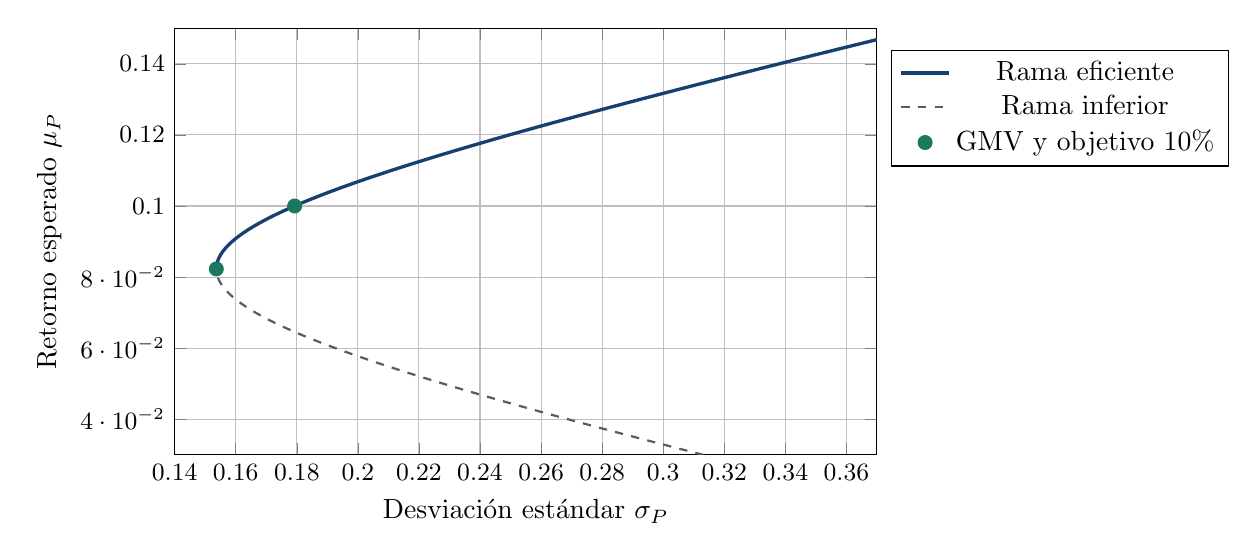
\begin{tikzpicture}
\begin{axis}[width=10.5cm,height=7cm,xlabel={Desviación estándar $\sigma_P$},ylabel={Retorno esperado $\mu_P$},grid=major,xmin=.14,xmax=.37,ymin=.03,ymax=.15,legend style={at={(1.02,.95)},anchor=north west},scaled ticks=false,tick label style={font=\small}]
\addplot[azul,very thick,domain=.08229508:.15,samples=120]({sqrt(36/1525+(1525/56)*(x-251/3050)^2)},{x});\addlegendentry{Rama eficiente}
\addplot[gris,dashed,thick,domain=.03:.08229508,samples=100]({sqrt(36/1525+(1525/56)*(x-251/3050)^2)},{x});\addlegendentry{Rama inferior}
\addplot[only marks,verde,mark=*,mark size=2.5pt]coordinates{(.15364426,.08229508)(.17928429,.10)};\addlegendentry{GMV y objetivo $10\%$}
\end{axis}\end{tikzpicture}
\caption{Frontera del ejemplo de tres activos con pesos reales y sin restricciones adicionales. La parte superior ofrece mayor retorno para cada nivel de riesgo de la frontera.}
\end{figure}
\subsection{Restricciones de no negatividad y caso singular}
Si $w_j\ge0$, las condiciones KKT para el objetivo $w\T\Sigma w/2$ son
\[
\Sigma w-\eta\ones_p-\gamma\mu-\nu=0,\quad
w\ge0,\quad\nu\ge0,\quad\nu_jw_j=0,
\]
además de las igualdades. La frontera pasa a estar formada por tramos con distintos conjuntos de activos con peso positivo. Si $\Sigma$ es singular, la inversa anterior no existe; usar pseudoinversa sin estudiar factibilidad y direcciones nulas puede omitir soluciones o riesgos nulos. Una regularización positiva permite un problema bien condicionado, pero cambia el modelo de riesgo.

\section{Factores principales de riesgo y portafolios propios}
Escribe $\Sigma=V\Lambda V\T$ y define $f=V\T(R-\mu)\in\R^{p\times1}$, con $\Cov(f)=\Lambda$. Para un portafolio $w\in\R^{p\times1}$, sus exposiciones a esos factores son $b=V\T w\in\R^{p\times1}$. Entonces
\[
R_P-\mu_P=w\T(R-\mu)=b\T f,\qquad
\boxed{\sigma_P^2=\sum_{j=1}^p\lambda_jb_j^2}.
\]
Cada término es no negativo y mide la contribución de un modo ortogonal de riesgo. Un autovector $v_j$ puede interpretarse como una combinación de activos cuya varianza, bajo norma euclidiana uno, es $\lambda_j$.
\subsection{Caso de correlación equicorrelacionada}
Supón que todos los activos tienen desviación $\sigma$ y correlación común $\rho$:
\[
\Sigma=\sigma^2[(1-\rho)I_p+\rho\ones_p\ones_p\T],\qquad -\frac1{p-1}\le\rho\le1.
\]
Para $v_1=\ones_p/\sqrt p\in\R^{p\times1}$,
\[
\Sigma v_1=\sigma^2[1+(p-1)\rho]v_1.
\]
Para cualquier $v\perp\ones_p$, $\Sigma v=\sigma^2(1-\rho)v$. Si $\rho>0$, el modo común es el dominante y los otros $p-1$ modos son contrastes. Con $w=\ones_p/p$,
\[
\sigma_P^2=\sigma^2\left[\rho+\frac{1-\rho}{p}\right].
\]
Al crecer $p$, el término específico se diluye, pero el común tiende a $\sigma^2\rho$ si $\rho>0$. Esta identidad muestra por qué diversificar muchos activos correlacionados no elimina todo el riesgo.
\subsection{Invertir la covarianza amplifica los modos pequeños}
\[
\Sigma^{-1}=\sum_j\frac1{\lambda_j}v_jv_j\T,\qquad
w_{\mathrm{GMV}}=\frac{\sum_j\lambda_j^{-1}v_j(v_j\T\ones_p)}{\sum_j\lambda_j^{-1}(v_j\T\ones_p)^2}.
\]
Autovalores pequeños reciben pesos recíprocos grandes. Un error pequeño de estimación puede cambiar mucho los pesos. Por eso un excelente ajuste de covarianza dentro de muestra no asegura una cartera estable fuera de muestra.
\subsection{Modelo de factores y riesgo residual}
Retener únicamente $\Sigma_k=V_k\Lambda_kV_k\T$ produce una matriz singular para $k<p$ y asigna riesgo cero a las direcciones descartadas. Un optimizador podría explotar esos ceros artificiales. Una opción de modelado es
\[
\widetilde\Sigma=V_k\Lambda_kV_k\T+\tau(I_p-V_kV_k\T),\quad \tau>0,
\]
que reemplaza los autovalores descartados por $\tau$. Otra es un modelo $BFB\T+D$ con $B\in\R^{p\times k}$, $F\succ0$ de dimensión $k\times k$ y $D\succ0$ diagonal de dimensión $p\times p$. Es preciso especificar cómo se estima cada parte; no es una identidad automática de PCA.

\section{Sharpe, Rayleigh generalizado y blanqueamiento del riesgo}
Sea $m=\mu-r_f\ones_p\in\R^{p\times1}$ el vector de retornos esperados en exceso de una tasa $r_f$, y supón $\Sigma\succ0$, $m\ne0$. El cociente homogéneo
\[
\mathcal Q(w)=\frac{(m\T w)^2}{w\T\Sigma w},\qquad w\ne0,
\]
es el cuadrado del cociente retorno en exceso/desviación. Definiendo $a=\Sigma^{1/2}w$ y $b=\Sigma^{-1/2}m$, ambos en $\R^{p\times1}$,
\[
(m\T w)^2=(b\T a)^2\le\norm b_2^2\norm a_2^2
=(m\T\Sigma^{-1}m)(w\T\Sigma w).
\]
Por tanto, $\mathcal Q(w)\le m\T\Sigma^{-1}m$, con igualdad cuando $w\propto\Sigma^{-1}m$. Para el cociente con signo positivo se elige la orientación con $m\T w>0$.
\subsection{La ecuación propia generalizada}
Maximizar $w\T(mm\T)w$ bajo $w\T\Sigma w=1$ produce
\[
\boxed{(mm\T)w=\rho\Sigma w},\qquad \rho=m\T\Sigma^{-1}m\text{ en el máximo}.
\]
$mm\T\in\R^{p\times p}$ tiene rango uno. Al blanquear $u=\Sigma^{1/2}w\in\R^{p\times1}$ se obtiene un problema propio ordinario para
\[
\Sigma^{-1/2}mm\T\Sigma^{-1/2}=bb\T.
\]
Si $\ones_p\T\Sigma^{-1}m\ne0$, se puede imponer presupuesto con
\[
w_T=\frac{\Sigma^{-1}m}{\ones_p\T\Sigma^{-1}m}.
\]
La orientación del retorno en exceso, las restricciones de cortos y la existencia de una tasa libre de riesgo importan para su interpretación como cartera tangente; el cociente al cuadrado por sí solo no distingue un retorno positivo de uno negativo.
\begin{idea}[La conexión completa solicitada]
PCA maximiza $v\T\Sigma v$ bajo $v\T v=1$ y da $\Sigma v=\lambda v$. Markowitz minimiza $w\T\Sigma w$ bajo presupuesto y retorno, dando $\Sigma w=\eta\ones_p+\gamma\mu$. Sharpe al cuadrado conduce a $(mm\T)w=\rho\Sigma w$. Los tres problemas comparten formas cuadráticas, proyecciones y teoría espectral, pero sus restricciones y objetivos no son iguales.
\end{idea}

\parte{VI. Extensiones: otras geometrías y otras nociones de información}
\section{PCA ponderado y autovalores generalizados}
\subsection{Ponderar observaciones}
Sean pesos $\pi_i>0$ con $\sum_i\pi_i=1$ y $\Omega=\diag(\pi_1,\ldots,\pi_n)\in\R^{n\times n}$. Define
\[
\mu_\pi=\sum_i\pi_i x_i\in\R^{p\times1},\quad
X_\pi=X-\ones_n\mu_\pi\T\in\R^{n\times p},\quad
S_\pi=X_\pi\T\Omega X_\pi\in\R^{p\times p}.
\]
Entonces $v\T S_\pi v=\sum_i\pi_i[v\T(x_i-\mu_\pi)]^2$. PCA de esta distribución empírica ponderada se calcula haciendo SVD de $\Omega^{1/2}X_\pi$. Su normalización es probabilística; una corrección de insesgamiento adicional depende de qué representen los pesos y no se asume automáticamente.
\subsection{Ponderar variables mediante una métrica}
Sea $M\succ0$, $M\in\R^{p\times p}$, y usemos la distancia $\norm{x-y}_M^2=(x-y)\T M(x-y)$. Transformar $y_i=M^{1/2}(x_i-\bar x)\in\R^{p\times1}$ convierte esa distancia en euclidiana. La covarianza transformada es
\[
S_y=M^{1/2}SM^{1/2}\in\R^{p\times p}.
\]
Si $a_j$ es autovector unitario de $S_y$, la dirección de reconstrucción original es $b_j=M^{-1/2}a_j\in\R^{p\times1}$, con $b_i\T Mb_j=\delta_{ij}$. Para $B_k=[b_1\ \cdots\ b_k]$,
\[
z_i=B_k\T M(x_i-\bar x),\quad
\widehat x_i=\bar x+B_kB_k\T M(x_i-\bar x).
\]
El proyector $P_M=B_kB_k\T M$ puede no ser simétrico en Euclides, pero cumple $P_M^2=P_M$ y $P_M\T M=MP_M$: es ortogonal respecto a la métrica $M$.
\subsection{Teorema para una restricción cuadrática general}
Si $A=A\T$ y $B\succ0$, ambos de dimensión $p\times p$,
\[
\max_{v\T Bv=1}v\T Av\quad\Longrightarrow\quad Av=\lambda Bv.
\]
Con $u=B^{1/2}v\in\R^{p\times1}$,
\[
v\T Av=u\T(B^{-1/2}AB^{-1/2})u,\qquad u\T u=1.
\]
La matriz interior es simétrica. Por el teorema espectral tiene autovalores reales y una base ortonormal $\{u_j\}$. Al volver, $v_j=B^{-1/2}u_j$ satisface $v_i\T Bv_j=\delta_{ij}$. Esta es la razón matemática de la ortogonalidad \emph{generalizada}.

\section{Discriminante lineal y correlación canónica: ejes con otro objetivo}
\subsection{LDA: separar clases en lugar de explicar variación total}
Sean dos clases con medias $\mu_1,\mu_2\in\R^{p\times1}$ y una matriz de dispersión interna $S_W\succ0$. Define $d=\mu_1-\mu_2\in\R^{p\times1}$. Fisher propone maximizar
\[
J(v)=\frac{[v\T(\mu_1-\mu_2)]^2}{v\T S_Wv}
=\frac{v\T dd\T v}{v\T S_Wv},\qquad v\ne0.
\]
Al blanquear $u=S_W^{1/2}v$ y aplicar Cauchy--Schwarz, el máximo es $d\T S_W^{-1}d$, alcanzado cuando $v\propto S_W^{-1}d$. La condición es $dd\T v=\lambda S_Wv$. LDA usa etiquetas y busca separación relativa a dispersión interna; PCA no usa etiquetas.
\begin{ejemplo}[PCA y LDA pueden elegir ejes perpendiculares]
Supón que ambas clases tienen covarianza interna $\diag(100,1)$, pero medias $(0,2)\T$ y $(0,-2)\T$. Con clases equiprobables, la covarianza total es $\diag(100,5)$. PCA elige el eje horizontal, porque $100>5$. LDA elige el vertical, ya que $d=(0,4)\T$ y $S_W^{-1}d=(0,4)\T$ si se usa esa covarianza interna. La separación de clases ocurre donde PCA ve menos varianza.
\end{ejemplo}
\begin{figure}[H]\centering
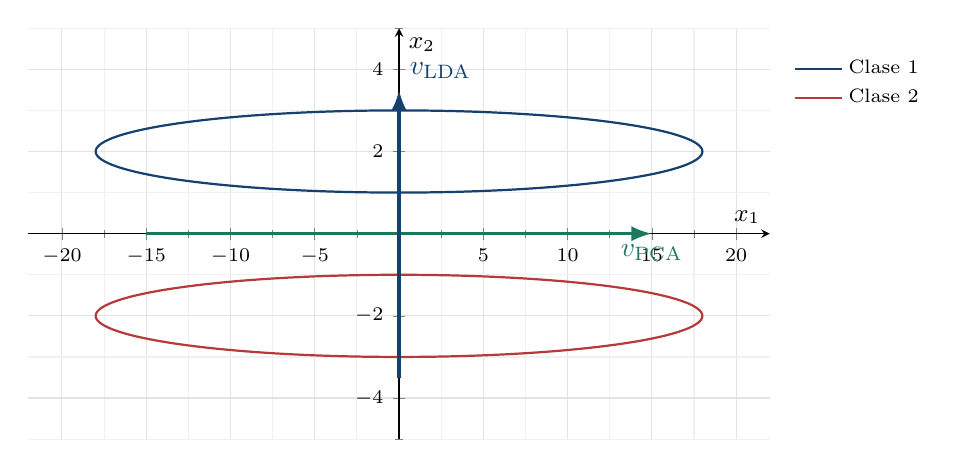
\begin{tikzpicture}
\begin{axis}[base,width=11cm,height=6.8cm,xmin=-22,xmax=22,ymin=-5,ymax=5,xlabel={$x_1$},ylabel={$x_2$},legend style={at={(1.02,.95)},anchor=north west}]
\addplot[azul,thick,domain=0:360]({18*cos(x)},{2+sin(x)});\addlegendentry{Clase 1}
\addplot[rojo,thick,domain=0:360]({18*cos(x)},{-2+sin(x)});\addlegendentry{Clase 2}
\draw[vecverde](axis cs:-15,0)--(axis cs:15,0)node[below]{$v_{\mathrm{PCA}}$};
\draw[vec](axis cs:0,-3.5)--(axis cs:0,3.5)node[above right]{$v_{\mathrm{LDA}}$};
\end{axis}\end{tikzpicture}
\caption{Esquema de clases alargadas horizontalmente pero separadas verticalmente. Las elipses ilustran la geometría; no representan una muestra ni un nivel probabilístico concreto.}
\end{figure}
\subsection{CCA: maximizar relación entre dos bloques}
Sean $x\in\R^{p\times1}$ y $y\in\R^{q\times1}$ aleatorios centrados, con covarianzas $\Sigma_{xx}\succ0$, $\Sigma_{yy}\succ0$ y cruzada $\Sigma_{xy}\in\R^{p\times q}$. CCA busca $a\in\R^{p\times1}$ y $b\in\R^{q\times1}$ que maximicen
\[
a\T\Sigma_{xy}b\quad\text{sujeto a }a\T\Sigma_{xx}a=1,\quad b\T\Sigma_{yy}b=1.
\]
Con $u=\Sigma_{xx}^{1/2}a$ y $v=\Sigma_{yy}^{1/2}b$, el problema es $\max_{\norm u=\norm v=1}u\T Kv$, donde
\[
K=\Sigma_{xx}^{-1/2}\Sigma_{xy}\Sigma_{yy}^{-1/2}\in\R^{p\times q}.
\]
La SVD $K=UDV\T$ muestra que el máximo es su mayor valor singular, $\rho_1$, y los pares siguientes usan sus restantes vectores singulares. Eliminando $b$ de las condiciones $\Sigma_{xy}b=\rho\Sigma_{xx}a$ y $\Sigma_{yx}a=\rho\Sigma_{yy}b$,
\[
\Sigma_{xy}\Sigma_{yy}^{-1}\Sigma_{yx}a=\rho^2\Sigma_{xx}a.
\]
Otra vez aparece una ecuación propia generalizada, pero aquí los autovalores son correlaciones canónicas al cuadrado.

\section{Kernel PCA: no lineal en los datos, lineal en características}
Sea $\phi:\R^p\to\mathcal H$ un mapa a un espacio de Hilbert con producto interno $\ip{\cdot}{\cdot}_{\mathcal H}$. Un núcleo válido satisface
\[
\kappa(x,y)=\ip{\phi(x)}{\phi(y)}_{\mathcal H},\qquad
K_{i\ell}=\kappa(x_i,x_\ell),\quad K\in\R^{n\times n},\quad K\succeq0.
\]
Se puede calcular PCA en $\mathcal H$ usando solo productos internos; no hace falta escribir cada coordenada de $\phi$. Este es el principio de kernel PCA.
\subsection{Centrar en el espacio correcto}
Define $\bar\phi=n^{-1}\sum_i\phi(x_i)$ y $\phi_c(x_i)=\phi(x_i)-\bar\phi$. La matriz de Gram centrada es
\[
\boxed{K_c=HKH},\qquad H=I_n-\frac1n\ones_n\ones_n\T,
\]
\[
(K_c)_{i\ell}=K_{i\ell}-\frac1n\sum_aK_{ia}-\frac1n\sum_aK_{a\ell}+\frac1{n^2}\sum_{a,b}K_{ab}.
\]
Centrar los datos $x_i$ no centra necesariamente $\phi(x_i)$ si $\phi$ es no lineal.
\subsection{Del operador de covarianza a la matriz de Gram}
Usamos el denominador $n$ en esta sección. El operador empírico es
\[
C_{\mathcal H}h=\frac1n\sum_i\phi_c(x_i)\ip{\phi_c(x_i)}h_{\mathcal H},\qquad h\in\mathcal H.
\]
Cualquier autovector $u\in\mathcal H$ de autovalor $\lambda>0$ pertenece al span de los $\phi_c(x_i)$ porque $u=\lambda^{-1}C_{\mathcal H}u$. Si $K_cq_j=\eta_jq_j$, $q_j\in\R^{n\times1}$ unitario y $\eta_j>0$, define
\[
u_j=\frac1{\sqrt{\eta_j}}\sum_i(q_j)_i\phi_c(x_i)\in\mathcal H.
\]
Entonces
\[
\norm{u_j}_{\mathcal H}^2=\frac{q_j\T K_cq_j}{\eta_j}=1,\qquad
C_{\mathcal H}u_j=\frac{\eta_j}{n}u_j.
\]
La puntuación de la observación $i$ es
\[
z_{ij}=\ip{\phi_c(x_i)}{u_j}_{\mathcal H}
=\frac{(K_cq_j)_i}{\sqrt{\eta_j}}=\sqrt{\eta_j}(q_j)_i.
\]
Así, autovalor de Gram $\eta_j$, varianza empírica $\eta_j/n$ y normalización del eje $1/\sqrt{\eta_j}$ son tres cantidades relacionadas, pero diferentes.
\subsection{Transformar un punto nuevo}
Para $x\in\R^{p\times1}$, define $k_c(x)\in\R^{n\times1}$ con entradas
\[
[k_c(x)]_i=\kappa(x_i,x)-\frac1n\sum_a\kappa(x_a,x)
-\frac1n\sum_aK_{ia}+\frac1{n^2}\sum_{a,b}K_{ab}.
\]
Entonces $z_j(x)=q_j\T k_c(x)/\sqrt{\eta_j}$. Todas las medias se refieren al conjunto de entrenamiento. Volver de una proyección en $\mathcal H$ a un punto original es el problema de preimagen; puede no tener solución exacta ni única.
\begin{ejemplo}[Núcleo cuadrático con mapa explícito]
Para $x=(x_1,x_2)\T\in\R^{2\times1}$,
\[
\phi(x)=(x_1^2,\sqrt2x_1x_2,x_2^2)\T\in\R^{3\times1},\quad
\phi(x)\T\phi(y)=x_1^2y_1^2+2x_1x_2y_1y_2+x_2^2y_2^2=(x\T y)^2.
\]
Una relación no lineal como $x_1^2+x_2^2=r^2$ se vuelve una relación lineal entre la primera y tercera características. Esto demuestra la posibilidad de linealizar estructura; no garantiza que la primera componente de cualquier núcleo separe automáticamente grupos concéntricos.
\end{ejemplo}
\subsection{Cálculo exacto con cuatro puntos}
Sean $x_1=(1,0)\T$, $x_2=(-1,0)\T$, $x_3=(0,1)\T$, $x_4=(0,-1)\T$. Para $\kappa(x,y)=(x\T y)^2$,
\[
K=\begin{pmatrix}1&1&0&0\\1&1&0&0\\0&0&1&1\\0&0&1&1\end{pmatrix},\quad
K_c=\frac12\begin{pmatrix}1&1&-1&-1\\1&1&-1&-1\\-1&-1&1&1\\-1&-1&1&1\end{pmatrix}.
\]
Hay un único autovalor positivo $\eta_1=2$, con $q_1=(1,1,-1,-1)\T/2$. Las puntuaciones son
\[
z_1=\sqrt2q_1=(1,1,-1,-1)\T/\sqrt2\in\R^{4\times1},\quad
\lambda_1(C_{\mathcal H})=\frac24=\frac12.
\]
El eje en características es $u_1=(1,0,-1)\T/\sqrt2$, por lo que $z(x)=(x_1^2-x_2^2)/\sqrt2$. Los puntos opuestos tienen la misma representación: el núcleo cuadrático no distingue $x$ de $-x$.

\section{MDS clásico: recuperar PCA a partir de distancias}
Supongamos que solo se conocen distancias euclidianas entre observaciones: $\delta_{ij}=\norm{x_i-x_j}_2$. Sea $D^{(2)}=(\delta_{ij}^2)\in\R^{n\times n}$. El escalamiento multidimensional clásico construye
\[
\boxed{B=-\frac12HD^{(2)}H\in\R^{n\times n}}.
\]
\begin{deduccion}
Sea $G=XX\T$ y $g=(G_{11},\ldots,G_{nn})\T\in\R^{n\times1}$. La identidad
\[
\delta_{ij}^2=\norm{x_i}_2^2+\norm{x_j}_2^2-2x_i\T x_j
\]
da $D^{(2)}=g\ones_n\T+\ones_ng\T-2G$. Como $H\ones_n=0$,
\[
-\frac12HD^{(2)}H=HGH=HXX\T H=X_cX_c\T.
\]
Si $X_c=U_rD_rV_r\T$, entonces $B=U_rD_r^2U_r\T$. Sus coordenadas de MDS son $Y_k=U_kD_k=X_cV_k$, exactamente las puntuaciones PCA, salvo rotaciones dentro de empates y signos.
\end{deduccion}
\subsection{Qué se puede recuperar y qué no}
Las distancias no determinan la traslación, rotación o reflexión del sistema original; sí determinan su geometría euclidiana hasta esas transformaciones cuando hay información suficiente. Si las disimilitudes no son euclidianas, $B$ puede tener autovalores negativos. Descartarlos aproxima otra geometría, pero ya no reproduce exactamente esas disimilitudes.
\subsection{Isomap y la diferencia entre distancia recta y distancia sobre una superficie}
Isomap sustituye distancias euclidianas por distancias de caminos mínimos en un grafo de vecinos y después aplica MDS. Busca aproximar distancias geodésicas de una variedad. Su resultado depende de que el grafo capture bien vecindades; atajos entre pliegues o componentes desconectados pueden alterar fuertemente la representación. Esta sección presenta el principio, no una garantía general de recuperación de variedades.

\section{Proyecciones aleatorias y conservación probabilística de distancias}
PCA elige ejes a partir de la covarianza. Una proyección aleatoria puede preservar aproximadamente todas las distancias de un conjunto finito sin estimar esos ejes. Sea $R\in\R^{k\times p}$ con entradas independientes $N(0,1/k)$ y define $f(x)=Rx\in\R^{k\times1}$.
\subsection{Una dirección fija y una variable chi-cuadrado}
Para $d\in\R^{p\times1}\setminus\{0\}$ fijo, cada entrada de $Rd$ es $N(0,\norm d_2^2/k)$ y son independientes. Por tanto,
\[
\frac{\norm{Rd}_2^2}{\norm d_2^2}\ \overset{d}=\ \frac{Y}{k},\qquad Y\sim\chi_k^2.
\]
En particular, $\E\norm{Rd}_2^2=\norm d_2^2$. Preservar en esperanza no basta; necesitamos concentración.
\subsection{Cota de concentración: derivación por Chernoff}
La función generadora de momentos es $\E e^{tY}=(1-2t)^{-k/2}$ para $t<1/2$. Para $0<\varepsilon<1$ y $t>0$,
\[
\Pr\{Y\ge k(1+\varepsilon)\}\le e^{-tk(1+\varepsilon)}(1-2t)^{-k/2}.
\]
Se minimiza con $t=\varepsilon/[2(1+\varepsilon)]$, dando
\[
\Pr\{Y\ge k(1+\varepsilon)\}\le
\exp\left[-\frac k2(\varepsilon-\log(1+\varepsilon))\right]
\le\exp\left[-k\left(\frac{\varepsilon^2}4-\frac{\varepsilon^3}6\right)\right].
\]
La última cota usa $\log(1+\varepsilon)\le\varepsilon-\varepsilon^2/2+\varepsilon^3/3$. El mismo argumento con $t<0$ produce una cota inferior al menos tan fuerte para la cola baja. Combinándolas,
\[
\Pr\left\{\left|\frac{\norm{Rd}_2^2}{\norm d_2^2}-1\right|>\varepsilon\right\}
\le2\exp\left[-k\left(\frac{\varepsilon^2}4-\frac{\varepsilon^3}6\right)\right].
\]
\subsection{De un par a todos los pares: lema de Johnson--Lindenstrauss}
Para $N$ puntos hay $M=N(N-1)/2$ pares. Por la cota de la unión, si
\[
k\ge\frac{\log(2M/\delta)}{\varepsilon^2/4-\varepsilon^3/6},\qquad0<\delta<1,
\]
con probabilidad al menos $1-\delta$ todas sus distancias cuadradas cumplen
\[
(1-\varepsilon)\norm{x_i-x_j}_2^2\le\norm{Rx_i-Rx_j}_2^2
\le(1+\varepsilon)\norm{x_i-x_j}_2^2.
\]
La dependencia es del orden $\varepsilon^{-2}\log(N/\delta)$, no lineal en $p$. La cota suficiente puede ser conservadora e incluso dar $k\ge p$ para tolerancias estrictas; no promete compresión útil en todo problema.
\begin{cuidado}[Objetivos diferentes]
PCA es óptimo para reconstrucción cuadrática mediante proyección ortogonal de rango fijo. Una proyección gaussiana reescalada no es generalmente ortogonal ni minimiza ese error, pero ofrece una garantía probabilística uniforme sobre distancias de un conjunto finito. Ninguno de estos enunciados domina al otro en todos los usos.
\end{cuidado}

\section{Grafos, Laplacianos y mapas no lineales}
\subsection{Otra ecuación espectral: conservar vecindades}
Sea $W=(w_{ij})\in\R^{n\times n}$ una matriz simétrica de pesos no negativos de un grafo, $D=\diag(d_1,\ldots,d_n)$ con $d_i=\sum_jw_{ij}$, y $L=D-W$. Para $y=(y_1,\ldots,y_n)\T\in\R^{n\times1}$,
\[
\boxed{y\T Ly=\frac12\sum_{i,j}w_{ij}(y_i-y_j)^2\ge0}.
\]
\textbf{Demostración.} Expandir los cuadrados da $\frac12\sum_{ij}w_{ij}(y_i^2+y_j^2-2y_iy_j)=\sum_i d_i y_i^2-\sum_{ij}w_{ij}y_iy_j$. Por simetría esto coincide con $y\T(D-W)y$.

Suponiendo $d_i>0$ (sin nodos aislados), minimizar esta energía con $y\T Dy=1$ y $y\T D\ones_n=0$ conduce a $Ly=\lambda Dy$. Se usan autovalores pequeños no triviales para ubicar cerca los nodos fuertemente conectados. En PCA se retienen autovalores \emph{grandes} de una covarianza; aquí pequeños de un Laplaciano: el significado del operador importa.
\subsection{Una cadena de tres nodos}
Para pesos unitarios entre 1--2 y 2--3,
\[
L=\begin{pmatrix}1&-1&0\\-1&2&-1\\0&-1&1\end{pmatrix},\quad
L(1,1,1)\T=0,\quad L(1,0,-1)\T=(1,0,-1)\T,
\]
\[
L(1,-2,1)\T=3(1,-2,1)\T.
\]
En la versión no normalizada con $y\T y=1$, el primer autovector no constante ordena los nodos como $1,0,-1$: representa la cadena en una recta. El autovalor cero corresponde a la coordenada constante y no aporta separación.
\subsection{t-SNE y UMAP: alcance de la comparación}
\textbf{t-SNE} transforma cercanías entre observaciones en probabilidades $p_{ij}$ y ajusta coordenadas $y_i\in\R^{k\times1}$ con afinidades $q_{ij}$ basadas en una distribución de colas pesadas. Minimiza $\sum_{i\ne j}p_{ij}\log(p_{ij}/q_{ij})$. Es una optimización no convexa de vecindades; sus ejes no son componentes principales y no tienen porcentajes de varianza explicada. El artículo original de van der Maaten y Hinton está en las referencias.

\textbf{UMAP} construye una representación ponderada de vecindades y optimiza una disposición en menor dimensión a partir de ella. Su planteamiento y parámetros difieren de t-SNE; tampoco se obtiene por diagonalizar la covarianza. Se remite al trabajo de McInnes, Healy y Melville para su construcción completa. En ambos casos, distancias entre grupos, tamaños visuales y huecos pueden depender fuertemente de parámetros y optimización; una figura separada no sustituye una comprobación estadística de grupos.
\begin{center}\small
\begin{tabular}{p{2.8cm}p{4.0cm}p{3.5cm}p{4.6cm}}\toprule
Método & Objeto principal & Estructura & Significado del eje\\\midrule
PCA & Covarianza & Lineal & Combinación de variables\\
Kernel PCA & Gram de características & No lineal en $x$ & Eje en un espacio de Hilbert\\
MDS clásico & Distancias al cuadrado & Euclidiana si es posible & Coordenada geométrica\\
Proyección aleatoria & Mapa aleatorio & Lineal & Dirección aleatoria reescalada\\
Laplaciano & Grafo de vecinos & Local & Función suave sobre nodos\\
t-SNE / UMAP & Afinidades de vecinos & No lineal & Coordenada del mapa ajustado\\\bottomrule
\end{tabular}\end{center}

\section{PCA en espacios de funciones: conexión directa con L2}
Sea $\mathcal H=L^2([0,1])$ con $\ip fg=\int_0^1f(t)g(t)\dd t$. Ahora una observación es una curva aleatoria $X\in\mathcal H$ y suponemos $\E\norm X_{\mathcal H}^2<\infty$. Su media es $m(t)=\E[X(t)]$ en el sentido apropiado de $L^2$. Definimos el operador de covarianza
\[
Cf=\E[\ip{X-m}f_{\mathcal H}(X-m)],\qquad f\in\mathcal H.
\]
Cuando se representa mediante un núcleo de covarianza,
\[
(Cf)(s)=\int_0^1K(s,t)f(t)\dd t,\qquad
K(s,t)=\Cov(X(s),X(t)).
\]
La integral hace el papel de la suma matricial. La ecuación propia es
\[
\boxed{\int_0^1K(s,t)\phi_j(t)\dd t=\lambda_j\phi_j(s)},\qquad
\int_0^1\phi_i(t)\phi_j(t)\dd t=\delta_{ij}.
\]
\subsection{Propiedades del operador}
\[
\ip{Cf}g=\E[\ip{X-m}f\ip{X-m}g]=\ip f{Cg},\qquad
\ip{Cf}f=\E[\ip{X-m}f^2]\ge0.
\]
Así, $C$ es autoadjunto y positivo. Bajo el segundo momento finito en un Hilbert separable, es de traza finita y compacto, con $\tr C=\E\norm{X-m}_{\mathcal H}^2$. El teorema espectral para operadores compactos positivos proporciona autovalores no negativos y funciones propias ortonormales en el soporte de la covarianza. La demostración completa de ese teorema funcional requiere análisis de operadores; aquí se explicitan sus consecuencias y la optimalidad de la truncación.
\subsection{Expansión de Karhunen--Loève y error de truncación}
Define puntuaciones aleatorias $\xi_j=\ip{X-m}{\phi_j}_{\mathcal H}\in\R$. Entonces
\[
\E[\xi_j]=0,\quad\E[\xi_i\xi_j]=\lambda_j\delta_{ij},\quad
X=m+\sum_{j\ge1}\xi_j\phi_j\quad\text{en }L^2(\Omega;\mathcal H),
\]
\[
\widehat X_k=m+\sum_{j=1}^k\xi_j\phi_j,\qquad
\boxed{\E\norm{X-\widehat X_k}_{\mathcal H}^2=\sum_{j>k}\lambda_j}.
\]
\textbf{Deducción del error.} Por ortogonalidad, la norma cuadrada del residuo es la suma de cuadrados de las coordenadas descartadas; tomar esperanza y usar Tonelli da $\sum_{j>k}\E\xi_j^2=\sum_{j>k}\lambda_j$. Para cualquier familia ortonormal $g_1,\ldots,g_k$, la varianza capturada es $\sum_\ell\ip{Cg_\ell}{g_\ell}$ y el mismo argumento de máxima traza da una cota $\sum_{j\le k}\lambda_j$. Por tanto, las funciones propias maximizan captura y minimizan error esperado.
\begin{ejemplo}[Un proceso de curvas con dos componentes exactas]
Sean $A,B$ aleatorios centrados, incorrelacionados, $\Var(A)=4$, $\Var(B)=1$. Define
\[
X(t)=A\phi_1(t)+B\phi_2(t),\quad
\phi_1(t)=1,\quad\phi_2(t)=\sqrt{12}(t-1/2),\quad0\le t\le1.
\]
Comprobamos $\int_0^1\phi_1^2=1$, $\int_0^1\phi_2^2=12(1/12)=1$ y $\int_0^1\phi_1\phi_2=0$. El núcleo es
\[
K(s,t)=4\phi_1(s)\phi_1(t)+\phi_2(s)\phi_2(t).
\]
Por integración, $C\phi_1=4\phi_1$ y $C\phi_2=\phi_2$. Retener solo $A\phi_1$ captura $4/5=80\%$ de variación integrada y deja error esperado uno. La primera componente cambia el nivel; la segunda, la pendiente.
\end{ejemplo}
\begin{figure}[H]\centering
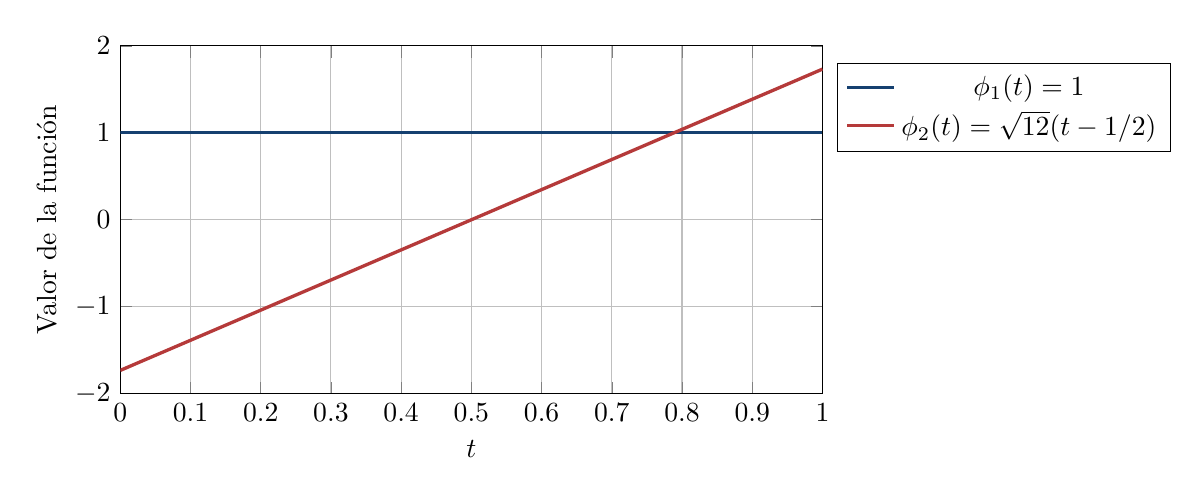
\begin{tikzpicture}
\begin{axis}[width=10.5cm,height=6cm,xlabel={$t$},ylabel={Valor de la función},xmin=0,xmax=1,ymin=-2,ymax=2,grid=major,legend style={at={(1.02,.95)},anchor=north west}]
\addplot[azul,very thick,domain=0:1]{1};\addlegendentry{$\phi_1(t)=1$}
\addplot[rojo,very thick,domain=0:1]{sqrt(12)*(x-.5)};\addlegendentry{$\phi_2(t)=\sqrt{12}(t-1/2)$}
\end{axis}\end{tikzpicture}
\caption{Funciones propias ortonormales en $L^2([0,1])$. El producto interno es una integral; no exige que las curvas sean perpendiculares como trazos en el papel.}
\end{figure}
\subsection{Discretizar una curva cambia la métrica si se ignoran los pesos}
Si una curva se mide en puntos $t_1,\ldots,t_p$ con pesos de cuadratura $\omega_j>0$, la integral se aproxima por $\sum_j\omega_jf(t_j)g(t_j)$. Definiendo $M=\diag(\omega_1,\ldots,\omega_p)$, se vuelve a PCA con métrica $M$. Hacer PCA ordinario sobre una malla irregular sin pesos puede dar importancia excesiva a regiones donde se midió más densamente.

\parte{VII. Cálculo numérico, estabilidad y variantes de PCA}
\section{Cómo calcular PCA sin confundir álgebra con cómputo}
\subsection{Ruta algebraica y ruta numérica}
Para matrices pequeñas, resolver $\det(S-\lambda I_p)=0$ enseña el significado de autovalores. Para matrices grandes, expandir el polinomio característico es una mala estrategia numérica. Una implementación usa algoritmos de autovalores simétricos o una SVD, no fórmulas de raíces de un polinomio de alto grado.

La ruta más directa con datos es: centrar, estandarizar si corresponde, calcular SVD, ordenar valores singulares, escoger $k$, formar puntuaciones y reconstruir. La SVD entrega los valores singulares no negativos en orden descendente en las implementaciones usuales, pero una rutina general de autovalores puede usar otro orden; hay que conservar emparejadas columnas y autovalores al reordenar.
\subsection{Por qué formar la covarianza puede perder precisión}
Si $X_c$ tiene valores singulares positivos $d_1\ge\cdots\ge d_r>0$, el condicionamiento sobre su rango es
\[
\kappa_2(X_c)=d_1/d_r,\qquad
\kappa_2(X_c\T X_c\text{ sobre su rango})=d_1^2/d_r^2=\kappa_2(X_c)^2.
\]
Si $X_c$ es singular, el condicionamiento de una inversa completa es infinito. La igualdad sobre el rango explica por qué elevar al cuadrado mediante $X_c\T X_c$ puede empeorar la separación numérica de valores muy pequeños. La SVD evita formar explícitamente ese producto.
\subsection{Costes y tolerancias}
Para una matriz densa $n\times p$, una SVD completa/económica cuesta del orden $np\min(n,p)$ operaciones. Si solo interesan unas pocas componentes, métodos iterativos o aleatorizados pueden reducir el coste. Los autovalores negativos diminutos que aparecen al diagonalizar una covarianza calculada en punto flotante pueden ser redondeo; negativos grandes obligan a revisar construcción, faltantes y simetría. No se deben cambiar signos arbitrariamente para esconder un problema.
\subsection{Qué comprobaciones tienen significado matemático}
Con ejes $V_k$, puntuaciones $Z_k$ y autovalores $\lambda_j$, comprobar
\[
\norm{V_k\T V_k-I_k}\F\approx0,\qquad
\norm{SV_k-V_k\Lambda_k}\F\approx0,
\]
\[
\norm{Z_k-X_cV_k}\F\approx0,\qquad
\norm{X_c-X_cV_kV_k\T}\F^2\approx(n-1)\sum_{j>k}\lambda_j.
\]
Las tolerancias deben escalar con magnitud y precisión numérica. Comparar signos de autovectores literalmente es una mala prueba; comparar proyectores $V_kV_k\T$ es apropiado cuando solo importa el subespacio.

\section{Método de la potencia, deflación y actualización en línea}
\subsection{Método de la potencia: prueba de convergencia direccional}
Sea $S\succeq0$, $\lambda_1>\lambda_2\ge0$ y $v^{(0)}\in\R^{p\times1}$ con componente no nula sobre $v_1$. Iteramos
\[
y^{(t+1)}=Sv^{(t)},\qquad v^{(t+1)}=\frac{y^{(t+1)}}{\norm{y^{(t+1)}}_2}.
\]
Si $v^{(0)}=\sum_j a_jv_j$ y $a_1\ne0$,
\[
S^tv^{(0)}=\lambda_1^t\left[a_1v_1+\sum_{j>1}a_j\left(\frac{\lambda_j}{\lambda_1}\right)^tv_j\right].
\]
Al normalizar, los términos restantes se anulan geométricamente; el límite es $\operatorname{sign}(a_1)v_1$. La rapidez depende de $\lambda_2/\lambda_1$: una brecha pequeña produce convergencia lenta. Si $a_1=0$, el método no puede recuperar esa componente en aritmética exacta.
\begin{ejemplo}[Dos iteraciones y la dirección límite]
Para $S=\begin{psmallmatrix}3&1\\1&3\end{psmallmatrix}$ y $v^{(0)}=(1,0)\T$,
\[
v^{(1)}=\frac{(3,1)\T}{\sqrt{10}},\qquad
v^{(2)}=\frac{(10,6)\T}{\sqrt{136}}=\frac{(5,3)\T}{\sqrt{34}},\qquad
v^{(t)}\longrightarrow\frac{(1,1)\T}{\sqrt2}.
\]
Los cocientes de Rayleigh son $3$, $3.6$ y $66/17\approx3.88235$, acercándose al autovalor máximo $4$.
\end{ejemplo}
\subsection{Deflación e iteración por subespacios}
Si se conocen exactamente $v_1,\lambda_1$, define $S^{(1)}=S-\lambda_1v_1v_1\T$. Entonces $S^{(1)}v_1=0$ y $S^{(1)}v_j=\lambda_jv_j$ para $j>1$. Repetir recupera otras componentes. En punto flotante, errores de deflación se acumulan; una iteración de subespacios actualiza simultáneamente $W\leftarrow SW$ y reortogonaliza sus columnas.
\subsection{Regla de Oja: una idea de PCA en línea}
Si llega una observación centrada $x_t\in\R^{p\times1}$, una actualización aproximada sobre la esfera es
\[
y_t=v_t\T x_t,\qquad
\widetilde v_{t+1}=v_t+\eta_t y_t(x_t-y_tv_t),\qquad
v_{t+1}=\frac{\widetilde v_{t+1}}{\norm{\widetilde v_{t+1}}_2}.
\]
En esperanza, el incremento sin normalizar es proporcional a $\Sigma v_t-(v_t\T\Sigma v_t)v_t$, que es el gradiente de Rayleigh proyectado al plano tangente de la esfera. La convergencia requiere condiciones sobre datos, pasos $\eta_t$ y brecha espectral; la fórmula sola no constituye una garantía universal. Si la media se estima en línea, también hay que actualizar el centrado.

\section{Perturbaciones: por qué un autovector puede cambiar mucho}
Sean $S$ y $\widehat S=S+E$ matrices simétricas $p\times p$, con $\norm E_2\le\varepsilon$. Para cualquier $v$ unitario,
\[
|v\T\widehat Sv-v\T Sv|=|v\T Ev|\le\norm E_2\le\varepsilon.
\]
Aplicando la caracterización min--max, se obtiene la cota de Weyl
\[
\boxed{|\widehat\lambda_j-\lambda_j|\le\varepsilon\quad\text{para todo }j.}
\]
Los autovalores son estables en error absoluto, pero los autovectores dependen también de separaciones entre autovalores.
\subsection{Cota del ángulo para la primera componente: prueba explícita}
Supón brecha $g=\lambda_1-\lambda_2>0$ y $\varepsilon<g/2$. Sean $v_1,\widehat v_1\in\R^{p\times1}$ unitarios, y $V_\perp=[v_2\ \cdots\ v_p]\in\R^{p\times(p-1)}$. Escribe
\[
\widehat v_1=a v_1+V_\perp b,\qquad b\in\R^{(p-1)\times1},\quad
\sin\theta=\norm b_2,
\]
eligiendo el signo para $a\ge0$. Proyectar $(S+E)\widehat v_1=\widehat\lambda_1\widehat v_1$ sobre el complemento da
\[
[\widehat\lambda_1 I_{p-1}-\diag(\lambda_2,\ldots,\lambda_p)]b
=V_\perp\T E\widehat v_1.
\]
Cada entrada diagonal del operador izquierdo es al menos $\lambda_1-\varepsilon-\lambda_2=g-\varepsilon>0$. Así,
\[
\boxed{\sin\theta\le\frac{\varepsilon}{g-\varepsilon}\le\frac{2\varepsilon}{g}}.
\]
Esta es una cota elemental del tipo de las cotas de perturbación de subespacios: ruido pequeño comparado con la brecha implica eje estable.
\begin{ejemplo}[Un cambio diminuto puede girar el eje noventa grados]
Sea $S=\diag(1.001,1)$ y $E=\diag(-0.002,0)$. Entonces $\norm E_2=0.002$, pequeño frente al nivel de los autovalores, pero mayor que la brecha $0.001$. El primer eje de $S$ es $(1,0)\T$; el de $\widehat S=\diag(0.999,1)$ es $(0,1)\T$. Cambió $90^\circ$ aunque los autovalores apenas cambiaron.
\end{ejemplo}
\subsection{Invariancia del subespacio cuando hay empates internos}
Si $\lambda_1\approx\lambda_2\gg\lambda_3$, los dos primeros ejes por separado pueden rotar mucho, pero el plano que generan puede ser estable. Para medir diferencias entre dos bases $V_k,\widehat V_k\in\R^{p\times k}$, se usan proyectores o ángulos principales: los valores singulares de $V_k\T\widehat V_k$ son $\cos\theta_1,\ldots,\cos\theta_k$.
\subsection{Muestra finita, consistencia y remuestreo}
Con dimensión $p$ fija, observaciones i.i.d. y segundos momentos finitos, cada entrada de $S$ converge a la correspondiente de $\Sigma$; en dimensión fija esto implica convergencia en norma. Si hay brecha positiva, los subespacios principales convergen. En alta dimensión, con $p$ creciendo con $n$, este argumento no basta. El bootstrap puede explorar variabilidad, pero debe volver a centrar y ajustar PCA en cada remuestra, alinear signos o subespacios y respetar dependencias temporales si existen.

\section{Ruido, robustez, dispersidad y matrices incompletas}
\subsection{Eliminar ruido no equivale a descartar siempre lo pequeño}
Si $X_c=L+N$ y $L$ tiene rango bajo, truncar SVD puede reducir parte del ruido de $N$. Pero si una señal importante vive en una dirección débil, también se pierde. El error óptimo de rango $k$ aproxima la \emph{matriz observada}; no prueba que se haya recuperado la matriz verdadera $L$.
\subsection{PCA robusto como suma de bajo rango y entradas dispersas}
Una formulación estudiada por Candès, Li, Ma y Wright plantea $X=L+S_0$ y resuelve
\[
\min_{L,S_0}\norm L_*+\alpha\norm{S_0}_1\quad\text{sujeto a }X=L+S_0,
\]
donde $\norm L_*=$ suma de valores singulares y $\norm{S_0}_1=\sum_{ij}|(S_0)_{ij}|$. La norma nuclear favorece bajo rango y la norma de entradas favorece corrupción dispersa. La recuperación exacta necesita supuestos de identificabilidad: una matriz que sea a la vez de bajo rango y muy dispersa puede asignarse ambiguamente a ambas partes. No es una garantía para cualquier tabla con atípicos. Con ruido pequeño adicional puede relajarse la igualdad mediante una tolerancia de Frobenius. El artículo original se cita al final.
\subsection{PCA disperso para interpretar pocas variables por eje}
Una formulación posible busca
\[
\max_{\norm v_2=1}v\T Sv-\alpha\norm v_1,\qquad v\in\R^{p\times1}.
\]
La penalización puede producir ejes con muchas coordenadas cero. La esfera hace el problema no convexo; no se resuelve simplemente diagonalizando $S$ y cambiando unos signos. Según la formulación, componentes sucesivas pueden no ser ortogonales o tener puntuaciones correlacionadas. Las propiedades deben comprobarse para el método concreto.
\subsection{Completar entradas faltantes mediante rango bajo}
Si $\mathcal O$ es el conjunto de entradas observadas, puede ajustarse
\[
\min_{A\in\R^{n\times k},\,B\in\R^{p\times k}}
\sum_{(i,j)\in\mathcal O}\left(x_{ij}-a_i\T b_j\right)^2
+\alpha(\norm A\F^2+\norm B\F^2),
\]
donde $a_i,b_j\in\R^{k\times1}$ son las traspuestas de las filas respectivas. Con todo observado y restricciones apropiadas reaparece la aproximación de rango bajo; con faltantes la SVD directa de la tabla incompleta no está definida. El patrón de observación y la validación sobre entradas ocultas son esenciales.
\subsection{SVD aleatorizada: compresión previa para acelerar}
Para $\ell=k+s$ con pequeño sobremuestreo $s$, se toma $\Omega\in\R^{p\times\ell}$ aleatoria y se calcula $Y=X_c\Omega\in\R^{n\times\ell}$. Una base ortonormal $Q\in\R^{n\times\ell}$ aproxima su rango; después se hace SVD de $B=Q\T X_c\in\R^{\ell\times p}$. Si $B=\widetilde UDV\T$, la aproximación es $Q\widetilde UDV\T$. Iteraciones de potencia pueden mejorar la separación cuando el espectro decae lentamente. La calidad depende del espectro, del sobremuestreo y del esquema; el análisis probabilístico completo se remite a Halko, Martinsson y Tropp.

\section{Laboratorio integral: doce observaciones y tres variables}
\label{sec:12datos}
Usamos ahora $n=12$, $p=3$ y una media no nula. La tabla no proviene de una base externa; fue construida para verificar exactamente el procedimiento.
\[
X=\begin{pmatrix}
53&83&10\\47&77&10\\51&79&10\\49&81&10\\52&82&10\\48&78&10\\
50&80&11\\50&80&9\\50&80&12\\50&80&8\\51&79&10\\49&81&10
\end{pmatrix}\in\R^{12\times3},\qquad
X_c=\begin{pmatrix}
3&3&0\\-3&-3&0\\1&-1&0\\-1&1&0\\2&2&0\\-2&-2&0\\
0&0&1\\0&0&-1\\0&0&2\\0&0&-2\\1&-1&0\\-1&1&0
\end{pmatrix}\in\R^{12\times3}.
\]
\subsection{Media y productos cruzados}
Las sumas de columnas son $600$, $960$, $120$, de modo que $\bar x=(50,80,10)\T\in\R^{3\times1}$. En los datos centrados,
\[
\sum_i x_{ci1}^2=2(9+1+4+1)=30,\quad
\sum_i x_{ci2}^2=30,\quad\sum_i x_{ci3}^2=2(1+4)=10,
\]
\[
\sum_i x_{ci1}x_{ci2}=2(9-1+4-1)=22,\qquad
\sum_i x_{ci1}x_{ci3}=\sum_i x_{ci2}x_{ci3}=0.
\]
Por tanto,
\[
X_c\T X_c=\begin{pmatrix}30&22&0\\22&30&0\\0&0&10\end{pmatrix},\quad
S=\frac1{11}\begin{pmatrix}30&22&0\\22&30&0\\0&0&10\end{pmatrix}.
\]
\subsection{Polinomio característico y orden correcto}
\[
\det(S-\lambda I_3)=\left(\frac{10}{11}-\lambda\right)
\left[\left(\frac{30}{11}-\lambda\right)^2-\left(\frac{22}{11}\right)^2\right].
\]
Las raíces son $52/11$, $8/11$ y $10/11$; \emph{ordenadas} de mayor a menor:
\[
\lambda_1=\frac{52}{11},\quad \lambda_2=\frac{10}{11},\quad \lambda_3=\frac8{11},
\quad v_1=\frac{(1,1,0)\T}{\sqrt2},\quad v_2=(0,0,1)\T,\quad
v_3=\frac{(1,-1,0)\T}{\sqrt2}.
\]
El segundo eje corresponde a la tercera variable original, porque su varianza $10/11$ supera la varianza del contraste entre las dos primeras, $8/11$.
\subsection{Puntuaciones y descomposición completa}
\[
V=\begin{pmatrix}1/\sqrt2&0&1/\sqrt2\\1/\sqrt2&0&-1/\sqrt2\\0&1&0\end{pmatrix},\quad
Z=X_cV=\begin{pmatrix}
3\sqrt2&0&0\\-3\sqrt2&0&0\\0&0&\sqrt2\\0&0&-\sqrt2\\2\sqrt2&0&0\\-2\sqrt2&0&0\\
0&1&0\\0&-1&0\\0&2&0\\0&-2&0\\0&0&\sqrt2\\0&0&-\sqrt2
\end{pmatrix}\in\R^{12\times3}.
\]
Las sumas de cuadrados de las columnas son $52$, $10$, $8$ y todos sus productos cruzados son cero. Los valores singulares son $\sqrt{52}=2\sqrt{13}$, $\sqrt{10}$ y $\sqrt8=2\sqrt2$; las columnas de $U$ se obtienen dividiendo cada columna de $Z$ por su valor singular.
\subsection{Retener uno, dos o tres ejes}
\begin{center}\small
\begin{tabular}{ccccc}\toprule
$k$ & Varianza acumulada & SSE & SSE$/12$ & Información descartada\\\midrule
1 & $52/70=74.2857\%$ & $18$ & $1.5$ & Tercera variable y contraste\\
2 & $62/70=88.5714\%$ & $8$ & $2/3$ & Contraste de variables 1 y 2\\
3 & $1=100\%$ & $0$ & $0$ & Ninguna\\\bottomrule
\end{tabular}\end{center}
Para $k=2$,
\[
P_2=V_2V_2\T=\begin{pmatrix}1/2&1/2&0\\1/2&1/2&0\\0&0&1\end{pmatrix},\qquad
\widehat x_i=\bar x+\left(\frac{x_{ci1}+x_{ci2}}2,\frac{x_{ci1}+x_{ci2}}2,x_{ci3}\right)\T.
\]
La observación 3, $(51,79,10)\T$, se reconstruye como $(50,80,10)\T$; su error cuadrado es dos. Ocurre lo mismo en las filas 4, 11 y 12. Las demás se reconstruyen exactamente: SSE$=4\cdot2=8$.
\subsection{¿Qué cambia al estandarizar?}
\[
D=\diag\left(\sqrt{30/11},\sqrt{30/11},\sqrt{10/11}\right),\quad
R=D^{-1}SD^{-1}=\begin{pmatrix}1&11/15&0\\11/15&1&0\\0&0&1\end{pmatrix}.
\]
Sus autovalores ordenados son $26/15$, $1$ y $4/15$, con los mismos ejes en coordenadas estandarizadas. Las proporciones pasan a
\[
\rho_1=\frac{26}{45}=57.7778\%,\quad\rho_2=\frac13=33.3333\%,\quad
\rho_3=\frac4{45}=8.8889\%,\quad C_2=\frac{41}{45}=91.1111\%.
\]
Estandarizar hace que la tercera variable represente una tercera parte de la variación inicial, en lugar de $10/70$. Incluso cuando los ejes mantienen su patrón, los porcentajes y el criterio para elegir $k$ pueden cambiar.
\subsection{Una observación nueva y sus dos reconstrucciones}
Para $x_*=(54,80,11)\T\in\R^{3\times1}$,
\[
x_{c,*}=(4,0,1)\T,\quad z_*=(2\sqrt2,1,2\sqrt2)\T,\quad
\widehat x_*^{(2)}=(52,82,11)\T,\quad\widehat x_*^{(1)}=(52,82,10)\T.
\]
Los errores cuadrados son $8$ y $9$. Se ve exactamente qué recupera añadir la segunda componente: la diferencia de una unidad en la tercera variable.

\section{Invariancias, información y afirmaciones que requieren condiciones}
\subsection{Traslación, escala común y rotación de los datos}
Si se suma $a\in\R^{p\times1}$ a cada observación, $X'=X+\ones_na\T$, entonces $X_c'=X_c$: PCA centrado es invariante a traslaciones. Si todos los datos se multiplican por $c\ne0$, la covarianza se multiplica por $c^2$: los subespacios y porcentajes no cambian.

Si $Q\in\R^{p\times p}$ es ortogonal y $Y_c=X_cQ$, entonces $S_Y=Q\T SQ$. Si $Sv_j=\lambda_jv_j$, se tiene $S_Y(Q\T v_j)=\lambda_j(Q\T v_j)$. Los autovalores no cambian y los ejes se transforman coherentemente. Cambiar unidades por factores distintos en cada columna no es una transformación ortogonal y no conserva generalmente PCA.
\subsection{No centrar puede hacer que domine la media}
\[
\frac1nX\T X=\frac1nX_c\T X_c+\bar x\bar x\T=S_n+\bar x\bar x\T.
\]
Si $\norm{\bar x}_2$ es grande, el segundo término puede dominar. Una SVD de $X$ sin centrar aproxima la tabla alrededor del origen; una SVD de $X_c$ aproxima fluctuaciones alrededor de la media. Ambos problemas son válidos, pero son distintos.
\begin{ejemplo}[Una media grande oculta la dirección de variación]
Para $X=\begin{psmallmatrix}100&-1\\100&0\\100&1\end{psmallmatrix}\in\R^{3\times2}$,
\[
\bar x=(100,0)\T,\quad X\T X=\diag(30000,2),\quad X_c\T X_c=\diag(0,2).
\]
Sin centrar, la primera dirección es horizontal y recoge principalmente el nivel constante 100. Con centrado, es vertical y recoge toda la variación observada.
\end{ejemplo}
\subsection{Entropía gaussiana de una proyección}
Si $\xi\sim N_p(0,\Sigma)$ con $\Sigma\succ0$ y $W\T W=I_k$, entonces $z=W\T\xi\in\R^{k\times1}$ tiene entropía diferencial
\[
h(z)=\frac12\log\left[(2\pi e)^k\det(W\T\Sigma W)\right].
\]
Sean $\theta_1\ge\cdots\ge\theta_k>0$ los autovalores de $W\T\Sigma W$. Por el principio min--max restringido al subespacio de $W$, $\theta_j\le\lambda_j(\Sigma)$. Así,
\[
\det(W\T\Sigma W)=\prod_{j=1}^k\theta_j\le\prod_{j=1}^k\lambda_j,
\]
y los primeros $k$ autovectores maximizan también esta entropía de salida entre proyecciones ortonormales. La conclusión usa normalidad y ese objetivo específico. ``Máxima información'' sin definir distribución, ruido y criterio puede ser una afirmación vacía; no equivale automáticamente a máxima información mutua con una etiqueta.
\subsection{PCA y bases de Hilbert: una comparación final}
Una base ortonormal cualquiera conserva energía al usar todas sus coordenadas, por Parseval. PCA elige una base ortonormal \emph{adaptada a la covarianza} para que las primeras coordenadas acumulen la mayor energía esperada. Fourier elige funciones por frecuencia; PCA funcional las elige por dispersión del proceso. Ambas permiten expansiones ortogonales, pero optimizan criterios distintos.

\parte{VIII. Taller resuelto: del cálculo elemental a la interpretación}
\section{Ejercicios 1--8: fundamentos, autovectores y geometría}
\begin{ejemplo}[1. Verificar una dirección propia sin determinantes]
\textbf{Problema.} Sean $A=\begin{psmallmatrix}2&1\\1&2\end{psmallmatrix}$ y $v=(1,-1)\T\in\R^{2\times1}$. ¿Es autovector? ¿Qué ocurre al normalizar?

\textbf{Solución.} $Av=(2-1,1-2)\T=(1,-1)\T=v$, por lo que $\lambda=1$. La norma es $\sqrt2$ y $q=v/\sqrt2$ cumple $Aq=q$, $q\T q=1$. La normalización cambia la longitud, no el autovalor. El vector $u=(1,0)\T$ no es propio porque $Au=(2,1)\T$ no es paralelo a $u$.
\end{ejemplo}
\begin{ejemplo}[2. Encontrar la otra dirección y reconstruir la matriz]
\textbf{Problema.} Diagonaliza la matriz del ejercicio 1.

\textbf{Solución.} $\det(A-\lambda I_2)=(2-\lambda)^2-1=(\lambda-3)(\lambda-1)$. Tomamos $q_1=(1,1)\T/\sqrt2$ y $q_2=(1,-1)\T/\sqrt2$, ambos en $\R^{2\times1}$. Son ortonormales y
\[
A=3q_1q_1\T+q_2q_2\T
=\frac32\begin{pmatrix}1&1\\1&1\end{pmatrix}+\frac12\begin{pmatrix}1&-1\\-1&1\end{pmatrix}
=\begin{pmatrix}2&1\\1&2\end{pmatrix}.
\]
La traza $4$ coincide con $3+1$ y el determinante $3$ con $3\cdot1$.
\end{ejemplo}
\begin{ejemplo}[3. Proyectar y medir exactamente lo perdido]
\textbf{Problema.} Proyecta $x=(4,0)\T\in\R^{2\times1}$ sobre $q_1=(1,1)\T/\sqrt2$.

\textbf{Solución.} La puntuación es $z=q_1\T x=2\sqrt2$. La proyección es $\widehat x=zq_1=(2,2)\T$ y el residuo $e=(2,-2)\T$. Por tanto $\norm{x}_2^2=16$, $\norm{\widehat x}_2^2=8$ y $\norm e_2^2=8$. La recta conserva la mitad de la energía de \emph{este punto}; eso no dice qué porcentaje conserva en una nube distinta.
\end{ejemplo}
\begin{ejemplo}[4. Covarianza de rango uno desde datos]
\textbf{Problema.} Usa $X=\begin{psmallmatrix}-1&-2\\0&0\\1&2\end{psmallmatrix}\in\R^{3\times2}$.

\textbf{Solución.} La media es cero y
\[
S=\frac12X\T X=\begin{pmatrix}1&2\\2&4\end{pmatrix},\quad
\det(S-\lambda I_2)=\lambda(\lambda-5).
\]
El eje positivo es $v_1=(1,2)\T/\sqrt5$, el nulo $v_2=(-2,1)\T/\sqrt5$, ambos en $\R^{2\times1}$. Las puntuaciones son $Z_1=(-\sqrt5,0,\sqrt5)\T\in\R^{3\times1}$ y $Z_1v_1\T=X$. Se conserva toda la información con una componente. El valor singular positivo es $\sqrt{(3-1)5}=\sqrt{10}$.
\end{ejemplo}
\begin{ejemplo}[5. Un empate no significa que el algoritmo esté mal]
\textbf{Problema.} ¿Cuáles son las componentes de $S=2I_3$?

\textbf{Solución.} Para cualquier $v\in\R^{3\times1}$, $Sv=2v$. Toda base ortonormal de $\R^3$ es una solución PCA. Cualquier eje captura $1/3$ de varianza; cualquier plano, $2/3$. Dos programas pueden devolver ejes diferentes con el mismo error óptimo. No existe una primera dirección identificada por la covarianza.
\end{ejemplo}
\begin{ejemplo}[6. Una matriz simétrica no tiene por qué ser covarianza]
\textbf{Problema.} ¿Puede $A=\begin{psmallmatrix}1&2\\2&1\end{psmallmatrix}$ ser una covarianza?

\textbf{Solución.} Tiene autovalores $3$ y $-1$. Para $v=(1,-1)\T/\sqrt2\in\R^{2\times1}$, $v\T Av=-1$. Una varianza no puede ser negativa, por lo que $A$ no es semidefinida positiva y no es una covarianza válida. La simetría sola no basta.
\end{ejemplo}
\begin{ejemplo}[7. Determinar la elipse a partir de sus autovalores]
\textbf{Problema.} Una covarianza tiene $v_1=(1,1)\T/\sqrt2$, $v_2=(1,-1)\T/\sqrt2$, con autovalores $9$ y $1$. Escribe $\Sigma$ y el contorno de Mahalanobis uno.

\textbf{Solución.} $\Sigma=9v_1v_1\T+v_2v_2\T=\begin{psmallmatrix}5&4\\4&5\end{psmallmatrix}$. En coordenadas $z=V\T x\in\R^{2\times1}$, el contorno es $z_1^2/9+z_2^2=1$; tiene semiejes $3$ y $1$. En coordenadas originales, $\Sigma^{-1}=\frac19\begin{psmallmatrix}5&-4\\-4&5\end{psmallmatrix}$ y el contorno es $(5x_1^2-8x_1x_2+5x_2^2)/9=1$.
\end{ejemplo}
\begin{ejemplo}[8. Dimensión máxima con pocas observaciones]
\textbf{Problema.} Hay cuatro observaciones y diez variables. ¿Cuántas componentes centradas pueden tener varianza positiva?

\textbf{Solución.} $X_c\in\R^{4\times10}$ y $X_c=HX$, con $\rank H=3$. Así, $\rank X_c\le3$ y $S\in\R^{10\times10}$ tiene al menos siete autovalores cero. Se pueden escribir diez autovectores, pero como máximo tres puntuaciones con varianza positiva. Obtener diez columnas de ejes no crea diez dimensiones informativas.
\end{ejemplo}

\section{Ejercicios 9--16: varianza, SVD, modelos y estabilidad}
\begin{ejemplo}[9. Elegir dimensión y calcular el error]
\textbf{Problema.} Para $n=21$, los autovalores son $(12,5,2,1)$. Elige el menor $k$ que conserve al menos $90\%$ y calcula SSE.

\textbf{Solución.} La suma es $20$; $C_1=0.60$, $C_2=0.85$, $C_3=0.95$. Por tanto $k=3$. La varianza residual es $1$, SSE$=(n-1)\cdot1=20$, error medio por observación $20/21$ y por celda $20/(21\cdot4)=5/21$. Los tres errores usan divisores distintos.
\end{ejemplo}
\begin{ejemplo}[10. Pasar de SVD a porcentajes]
\textbf{Problema.} Los valores singulares de una matriz centrada con $n=10$ son $6$, $3$ y $1$. Calcula autovalores y error al retener dos.

\textbf{Solución.} $\lambda=(36/9,9/9,1/9)\T=(4,1,1/9)\T\in\R^{3\times1}$, cuya suma es $46/9$. Las proporciones son $36/46$, $9/46$ y $1/46$. Retener dos conserva $45/46\approx97.8261\%$ y deja SSE$=1$. Cambiar $n-1$ por $n$ cambia las varianzas, pero no estos porcentajes ni la reconstrucción.
\end{ejemplo}
\begin{ejemplo}[11. Blanquear una covarianza diagonal]
\textbf{Problema.} Si $\Cov(z)=\diag(9,4,1)$, para $z\in\R^{3\times1}$ centrado, encuentra una variable blanqueada.

\textbf{Solución.} $w=(z_1/3,z_2/2,z_3)\T\in\R^{3\times1}$ tiene $\Cov(w)=I_3$. La transformación es invertible: $z=(3w_1,2w_2,w_3)\T$. Blanquear aquí no reduce dimensión; descartar alguna coordenada sería otra operación.
\end{ejemplo}
\begin{ejemplo}[12. Descartar una dirección puede colapsar una distancia]
\textbf{Problema.} Proyecta $x=(1,1)\T$ y $y=(1,-1)\T$ sobre el eje $e_1=(1,0)\T$, todos en $\R^{2\times1}$.

\textbf{Solución.} Las puntuaciones de ambos puntos son uno. La distancia original es $\norm{x-y}_2=2$ y la distancia proyectada es cero. Toda la diferencia $(0,2)\T$ está en el eje descartado. Aunque ese eje pudiera tener poca varianza en una base grande, este par pierde el $100\%$ de su separación.
\end{ejemplo}
\begin{ejemplo}[13. Un PCR calculado sin ecuaciones normales grandes]
\textbf{Problema.} En el ejemplo maestro, toma $y_c=(1,2,0,-1,-2,0)\T\in\R^{6\times1}$ y conserva una componente.

\textbf{Solución.} $u_1\T y_c=(1+2+0+1+2+0)/\sqrt6=\sqrt6$. Como $d_1=4\sqrt3$,
\[
\widehat\gamma=\frac{\sqrt6}{4\sqrt3}=\frac{\sqrt2}{4},\qquad
\widehat\beta=v_1\widehat\gamma=(1/4,1/4)\T\in\R^{2\times1}.
\]
Las predicciones centradas son $X_c\widehat\beta=(1,1,1,-1,-1,-1)\T$. Los residuos son $(0,1,-1,0,-1,1)\T$ y su suma de cuadrados es cuatro. El eje se estimó sin mirar $y_c$; luego se ajustó el coeficiente sobre las puntuaciones.
\end{ejemplo}
\begin{ejemplo}[14. Ruido estimado en PPCA]
\textbf{Problema.} Una covarianza con denominador $n$ tiene autovalores $(7,4,1,0.5)$. Ajusta PPCA con $k=2$.

\textbf{Solución.} $\widehat\sigma^2=(1+0.5)/2=0.75$. Una elección de cargas es $W=V_2\diag(\sqrt{6.25},\sqrt{3.25})\in\R^{4\times2}$. La covarianza ajustada tiene autovalores $(7,4,0.75,0.75)$: conserva los dos dominantes y reemplaza el resto por su promedio. No pone los autovalores descartados a cero.
\end{ejemplo}
\begin{ejemplo}[15. Autovalor generalizado con cálculo directo]
\textbf{Problema.} Maximiza $v\T Av$ sujeto a $v\T Bv=1$, con $A=\diag(9,4)$ y $B=\diag(4,1)$.

\textbf{Solución.} $B^{-1/2}AB^{-1/2}=\diag(9/4,4)$. El máximo es $4$ y corresponde a $u=(0,1)\T$, de donde $v=B^{-1/2}u=(0,1)\T\in\R^{2\times1}$. Con la restricción euclidiana $v\T v=1$, el máximo habría sido $9$ en la primera coordenada. Cambiar métrica cambia el problema.
\end{ejemplo}
\begin{ejemplo}[16. Cota cuantitativa de estabilidad]
\textbf{Problema.} Si $\lambda_1=10$, $\lambda_2=6$ y $\norm E_2\le0.2$, acota el cambio del primer autovalor y el ángulo del primer eje.

\textbf{Solución.} Weyl da $|\widehat\lambda_1-10|\le0.2$. La brecha es $g=4$ y $0.2<g/2$, por lo que $\sin\theta\le0.2/3.8=1/19\approx0.052632$. Así, $\theta\le\arcsin(1/19)\approx3.017^\circ$. La orientación de signo se alinea antes de medir el ángulo.
\end{ejemplo}

\section{Ejercicios 17--24: portafolios, núcleos y conexiones}
\begin{ejemplo}[17. Mínima varianza con activos incorrelacionados]
\textbf{Problema.} Calcula GMV para $\Sigma=\diag(9,1)$ y presupuesto uno.

\textbf{Solución.} $\Sigma^{-1}\ones_2=(1/9,1)\T$, cuya suma es $10/9$. Entonces $w=(1/10,9/10)\T\in\R^{2\times1}$ y $w\T\Sigma w=9/100+81/100=0.9$. Invertir todo en el segundo activo da riesgo uno. El autovector de menor varianza bajo norma unitaria es $(0,1)\T$, pero la solución de presupuesto reparte pesos y tiene norma menor que uno.
\end{ejemplo}
\begin{ejemplo}[18. Detectar una posición corta óptima]
\textbf{Problema.} Resuelve GMV para $\Sigma=\begin{psmallmatrix}1&2\\2&9\end{psmallmatrix}$, primero sin restricciones de signo y luego sin cortos.

\textbf{Solución.} La matriz es definida positiva porque su primer menor es uno y su determinante cinco. Con $w=(t,1-t)\T$,
\[
f(t)=t^2+9(1-t)^2+4t(1-t)=6t^2-14t+9.
\]
$f'(t)=12t-14=0$ da $t=7/6$, luego $w=(7/6,-1/6)\T$ y $f(t)=5/6$. Sin cortos, $0\le t\le1$; la parábola disminuye en ese intervalo, así que el mínimo está en $t=1$, riesgo uno. Renormalizar después de eliminar un peso negativo no es una demostración; aquí la restricción se resuelve explícitamente.
\end{ejemplo}
\begin{ejemplo}[19. Covarianza singular con muchos mínimos]
\textbf{Problema.} ¿Qué ocurre con $\Sigma=\begin{psmallmatrix}1&1\\1&1\end{psmallmatrix}$ y $w_1+w_2=1$?

\textbf{Solución.} $w\T\Sigma w=(w_1+w_2)^2=1$ para todo portafolio factible. Hay infinitos mínimos. La dirección nula $(1,-1)\T$ modifica pesos sin alterar riesgo ni presupuesto. La inversa no existe y no se puede aplicar la fórmula de GMV con una inversa ordinaria.
\end{ejemplo}
\begin{ejemplo}[20. Covarianza singular con riesgo cero factible]
\textbf{Problema.} Repite con $\Sigma=\begin{psmallmatrix}1&-1\\-1&1\end{psmallmatrix}$.

\textbf{Solución.} Ahora $w\T\Sigma w=(w_1-w_2)^2$. Bajo presupuesto uno, el mínimo cero se alcanza en $w=(1/2,1/2)\T\in\R^{2\times1}$. La dirección nula tiene suma distinta de cero y puede normalizarse como cartera. Una matriz singular puede producir situaciones muy diferentes según cómo su núcleo interactúe con las restricciones.
\end{ejemplo}
\begin{ejemplo}[21. Efecto de un modo común al aumentar activos]
\textbf{Problema.} Para $p=10$, $\sigma=0.20$ y correlación común $\rho=0.30$, calcula riesgo de pesos iguales y proporción de la primera componente.

\textbf{Solución.} $\lambda_1=0.04[1+9(0.3)]=0.148$ y los otros nueve autovalores son $0.04(0.7)=0.028$. La traza es $0.4$, así que PC1 explica $0.148/0.4=37\%$. El portafolio de pesos iguales tiene varianza $0.04[0.3+0.7/10]=0.0148$ y desviación $\sqrt{0.0148}\approx0.121655$. El autovector común tiene norma uno; los pesos iguales suman uno y son ese autovector dividido por $\sqrt{10}$.
\end{ejemplo}
\begin{ejemplo}[22. Riesgo por componentes]
\textbf{Problema.} En una base propia con $\Lambda=\diag(5,2,1)$, las exposiciones de un portafolio son $b=(0.2,-0.3,0.4)\T\in\R^{3\times1}$. Calcula las contribuciones.

\textbf{Solución.} La varianza es $5(0.2)^2+2(-0.3)^2+1(0.4)^2=0.20+0.18+0.16=0.54$. Las contribuciones relativas son $10/27$, $1/3$ y $8/27$. El signo negativo de una exposición no hace negativa su contribución de varianza en factores incorrelacionados. El vector $b$ no tiene por qué sumar uno: contiene exposiciones, no pesos originales.
\end{ejemplo}
\begin{ejemplo}[23. Verificar un núcleo por un mapa de características]
\textbf{Problema.} Para $x,y\in\R$, muestra que $\kappa(x,y)=(1+xy)^2$ es semidefinido positivo.

\textbf{Solución.} Usa $\phi(x)=(1,\sqrt2x,x^2)\T\in\R^{3\times1}$. Entonces $\phi(x)\T\phi(y)=1+2xy+x^2y^2=(1+xy)^2$. Para cualquier conjunto $x_1,\ldots,x_n$ y $a\in\R^{n\times1}$,
\[
a\T Ka=\sum_{i,j}a_ia_j\phi(x_i)\T\phi(x_j)=\norm{\sum_i a_i\phi(x_i)}_2^2\ge0.
\]
Esto verifica directamente la propiedad de Gram positiva sin inspeccionar todos los posibles conjuntos de datos.
\end{ejemplo}
\begin{ejemplo}[24. PCA funcional como cálculo de integrales]
\textbf{Problema.} Para $X(t)=A+\sqrt{12}B(t-1/2)$ del ejemplo funcional, con $\Var A=4$, $\Var B=1$ y covarianza cero, calcula las puntuaciones mediante integrales.

\textbf{Solución.} $\xi_1=\int_0^1X(t)\dd t=A$ porque $\int_0^1(t-1/2)\dd t=0$. Para la segunda,
\[
\xi_2=\int_0^1X(t)\sqrt{12}(t-1/2)\dd t
=12B\int_0^1(t-1/2)^2\dd t=B.
\]
La reconstrucción con una componente es la función constante $\widehat X_1(t)=A$. Su error integrado es $\int_0^1[X(t)-A]^2\dd t=B^2$, cuya esperanza es uno. Es exactamente el mismo patrón que una proyección vectorial, con integrales en lugar de sumas.
\end{ejemplo}

\section{Laboratorio reproducible en MATLAB: PCA por SVD}
El siguiente código reproduce el ejemplo de seis observaciones. Utiliza operaciones de MATLAB base y no necesita la función \texttt{pca}. La rutina \texttt{svd} calcula $X_c=UDV\T$; la documentación oficial se enlaza en las referencias. Los cálculos numéricos del documento se verificaron también mediante una implementación independiente.
\begin{lstlisting}[language=Matlab]
% PCA por SVD: n = 6 observaciones, p = 2 variables.
X = [12 22; 13 21; 11 23; 8 18; 7 19; 9 17];
[n,p] = size(X);
media = mean(X,1);                  % 1 x p
Xc = X - repmat(media,n,1);         % n x p
S = (Xc.' * Xc)/(n-1);             % p x p
[U,D,V] = svd(Xc,'econ');
d = diag(D);
lambda = d.^2/(n-1);

% Fijar un signo convencional sin cambiar la SVD.
for j = 1:size(V,2)
    [~,pos] = max(abs(V(:,j)));
    if V(pos,j) < 0
        V(:,j) = -V(:,j);
        U(:,j) = -U(:,j);
    end
end

Z = Xc * V;                        % n x p en este ejemplo
k = 1;
Vk = V(:,1:k);                     % p x k
Zk = Z(:,1:k);                     % n x k
Xc_est = Zk * Vk.';                % n x p
X_est = Xc_est + repmat(media,n,1);
E = Xc - Xc_est;
SSE = norm(E,'fro')^2;
fraccion = lambda/sum(lambda);
acumulada = cumsum(fraccion);

% Verificaciones con tolerancia, no igualdad literal.
assert(norm(V.'*V-eye(p),'fro') < 1e-10);
assert(norm(S*V-V*diag(lambda),'fro') < 1e-10);
assert(norm(Z-U*D,'fro') < 1e-10);
assert(abs(SSE-(n-1)*sum(lambda(k+1:end))) < 1e-10);

disp(S); disp(lambda); disp(Z); disp(X_est); disp(SSE);
% Valores esperados: lambda = [9.6; 1.6], SSE = 8.

% Aplicar el modelo ya ajustado a una observacion nueva.
xnuevo = [14 22];                   % 1 x p (fila de datos)
znuevo = (xnuevo-media)*Vk;         % 1 x k
xnuevo_est = znuevo*Vk.'+media;     % [13 23]
\end{lstlisting}
\subsection{Calcular una cartera resolviendo un sistema lineal}
Para evaluar $\Sigma^{-1}\ones_p$ no es necesario construir la inversa: se resuelve $\Sigma u=\ones_p$ y se normaliza.
\begin{lstlisting}[language=Matlab]
Sigma = [0.04 0.006; 0.006 0.09];
mu = [0.08; 0.14];
uno = ones(2,1);
u = Sigma \ uno;
w = u/(uno.'*u);
media_cartera = mu.'*w;
var_cartera = w.'*Sigma*w;
desv_cartera = sqrt(var_cartera);
% w = [0.7118644068; 0.2881355932]
% var_cartera = 0.03020338983
% desv_cartera = 0.17379122484
\end{lstlisting}
El bloque calcula el caso sin restricciones de signo adicionales. Para cotas o prohibición de cortos, la solución puede requerir un problema cuadrático restringido. Los datos de este laboratorio son hipotéticos.

\section{Cuadros de consulta: dimensiones y fórmulas esenciales}
\begin{center}\small
\begin{longtable}{p{2.7cm}p{2.4cm}p{9.8cm}}\toprule
Objeto & Dimensión & Significado\\\midrule\endhead
$x_i,\bar x$ & $p\times1$ & Observación y media como vectores columna\\
$X,X_c$ & $n\times p$ & Tabla original y centrada; observaciones en filas\\
$H$ & $n\times n$ & Proyector de centrado sobre suma cero\\
$S,\Sigma$ & $p\times p$ & Covarianzas muestral y poblacional\\
$v_j$ & $p\times1$ & Eje principal unitario\\
$V_k$ & $p\times k$ & Primeros $k$ ejes ortonormales\\
$\Lambda_k$ & $k\times k$ & Varianzas principales en diagonal\\
$z_i$ & $k\times1$ & Coordenadas de una observación\\
$z_j=X_cv_j$ & $n\times1$ & Puntuaciones de una componente en toda la muestra\\
$Z_k$ & $n\times k$ & Matriz de puntuaciones; fila $i$ igual a $z_i\T$\\
$P_k$ & $p\times p$ & Proyector $V_kV_k\T$\\
$U_r,D_r,V_r$ & $n\times r$, $r\times r$, $p\times r$ & Factores de la SVD compacta\\
$\widehat X,E$ & $n\times p$ & Datos reconstruidos y residuos\\
$w,\mu$ & $p\times1$ & Pesos financieros y retornos esperados\\
$K,K_c$ & $n\times n$ & Gram de núcleo antes y después de centrar\\\bottomrule
\end{longtable}\end{center}
\begin{idea}[Cadena de identidades para PCA muestral]
\begin{gather*}
X_c=X-\ones_n\bar x\T,\qquad S=\frac{X_c\T X_c}{n-1},\qquad
SV=V\Lambda,\qquad S=V\Lambda V\T,\\
X_c=U_rD_rV_r\T,\qquad\lambda_j=\frac{d_j^2}{n-1},\qquad
Z_k=X_cV_k=U_kD_k,\\
\widehat X=\ones_n\bar x\T+Z_kV_k\T,\qquad
\norm{X-\widehat X}\F^2=\sum_{j>k}d_j^2=(n-1)\sum_{j>k}\lambda_j.
\end{gather*}
\end{idea}
\begin{idea}[Cadena de identidades para portafolios]
\begin{gather*}
\Var(w\T R)=w\T\Sigma w=\sum_j\lambda_j(v_j\T w)^2,\\
\min_{w\T w=1}w\T\Sigma w=\lambda_{\min},\qquad
\max_{w\T w=1}w\T\Sigma w=\lambda_{\max},\\
w_{\mathrm{GMV}}=\frac{\Sigma^{-1}\ones_p}{\ones_p\T\Sigma^{-1}\ones_p},\qquad
\sigma_{\mathrm{GMV}}^2=\frac1{\ones_p\T\Sigma^{-1}\ones_p}\quad(\Sigma\succ0).
\end{gather*}
\end{idea}
\subsection{Diez errores conceptuales que este tratado permite detectar}
\begin{enumerate}
\item Decir que todo autovector maximiza: solo lo hace el autoespacio del mayor autovalor bajo la restricción correspondiente.
\item Confundir $v_j$ con $z_j$: uno pondera variables; el otro contiene puntuaciones de observaciones.
\item Confundir $d_j$ con $\lambda_j$: la varianza es $d_j^2/(n-1)$.
\item Omitir el centrado sin reconocer que se cambió el objetivo.
\item Tratar incorrelación como independencia sin una hipótesis suficiente.
\item Interpretar $95\%$ de varianza como $95\%$ de precisión predictiva.
\item Esperar que $V_k\T V_k=I_k$ implique $V_kV_k\T=I_p$ cuando $k<p$.
\item Suponer que blanqueamiento y PCA son la misma operación.
\item Afirmar que Markowitz siempre conduce a $\Sigma w=\lambda w$.
\item Invertir una covarianza truncada singular como si tuviera todos sus autovalores positivos.
\end{enumerate}

\section{Compilación en MiKTeX y VS Code}
El archivo fuente está guardado en UTF-8 y usa la misma familia de paquetes y el mismo estilo visual del ejemplo proporcionado: clase \texttt{article}, papel A4, márgenes de 1.8 cm, fuente de 11 puntos, recuadros, ecuaciones compactas y figuras vectoriales.
\begin{enumerate}
\item Guarda el archivo \texttt{.tex} en tu carpeta de trabajo y ábrelo en VS Code.
\item Compílalo con tu receta habitual de pdfLaTeX/LaTeX Workshop. Dos pasadas actualizan índice y referencias; \texttt{latexmk -pdf} las gestiona automáticamente.
\item El PDF se genera con el mismo nombre base del archivo \texttt{.tex}. Abre ese PDF para comprobar que estás viendo este documento.
\end{enumerate}
No hay instrucciones \texttt{\textbackslash input} para capítulos externos ni archivos de imágenes requeridos. Los bloques MATLAB se imprimen como texto: no se ejecutan durante la compilación. Los paquetes son los del preámbulo; MiKTeX debe disponer de ellos o permitir su instalación habitual si falta alguno. No se necesita cambiar un archivo de configuración del proyecto para utilizar este documento.
\begin{lstlisting}
pdflatex PCA_Teorema_Espectral_SVD_ML_Portafolios.tex
pdflatex PCA_Teorema_Espectral_SVD_ML_Portafolios.tex
\end{lstlisting}
También puede usarse una sola orden:
\begin{lstlisting}
latexmk -pdf PCA_Teorema_Espectral_SVD_ML_Portafolios.tex
\end{lstlisting}

\section{Referencias y rutas para continuar}
Las demostraciones, ejemplos numéricos y figuras de este documento están desarrollados para esta guía. Las siguientes fuentes sirven para contrastar fundamentos y profundizar en extensiones; no se han reproducido sus páginas ni sus figuras.
\begin{enumerate}[label={[\arabic*]},itemsep=5pt]
\item Shalizi, C. R. (2016). \textit{Principal Components Analysis}, capítulo de apuntes de análisis de datos, Carnegie Mellon University. Fundamentos geométricos y relación entre varianza y reconstrucción.\\
\href{https://www.stat.cmu.edu/~cshalizi/uADA/16/lectures/17.pdf}{Apuntes originales de PCA en Carnegie Mellon}.
\item Tipping, M. E. y Bishop, C. M. (1999). \textit{Probabilistic Principal Component Analysis}. Journal of the Royal Statistical Society, Series B, 61(3), 611--622. Modelo probabilístico de componentes principales.\\
\href{https://www.microsoft.com/en-us/research/publication/probabilistic-principal-component-analysis/}{Ficha del artículo en Microsoft Research}.
\item Schölkopf, B., Smola, A. y Müller, K.-R. (1998). \textit{Nonlinear Component Analysis as a Kernel Eigenvalue Problem}. Neural Computation, 10(5), 1299--1319. Referencia original de kernel PCA. DOI: \href{https://doi.org/10.1162/089976698300017467}{10.1162/089976698300017467}.
\item Markowitz, H. (1952). \textit{Portfolio Selection}. The Journal of Finance, 7(1), 77--91. Referencia fundacional de selección media--varianza. DOI: \href{https://doi.org/10.1111/j.1540-6261.1952.tb01525.x}{10.1111/j.1540-6261.1952.tb01525.x}.
\item van der Maaten, L. y Hinton, G. (2008). \textit{Visualizing Data using t-SNE}. Journal of Machine Learning Research, 9, 2579--2605.\\
\href{https://www.jmlr.org/papers/v9/vandermaaten08a.html}{Artículo original en JMLR}.
\item McInnes, L., Healy, J. y Melville, J. \textit{UMAP: Uniform Manifold Approximation and Projection for Dimension Reduction}. Prepublicación iniciada en 2018; versión revisada de 2020.\\
\href{https://arxiv.org/abs/1802.03426}{Trabajo original y versiones en arXiv}.
\item Candès, E. J., Li, X., Ma, Y. y Wright, J. \textit{Robust Principal Component Analysis?} Prepublicación de 2009; publicada en Journal of the ACM, 58(3), 2011.\\
\href{https://arxiv.org/abs/0912.3599}{Artículo sobre descomposición de bajo rango y corrupción dispersa}.
\item Halko, N., Martinsson, P. G. y Tropp, J. A. \textit{Finding Structure with Randomness: Probabilistic Algorithms for Constructing Approximate Matrix Decompositions}. Prepublicación de 2009; SIAM Review, 53(2), 2011.\\
\href{https://arxiv.org/abs/0909.4061}{Fundamentos de aproximaciones matriciales aleatorizadas}.
\item MathWorks. Documentación oficial de \href{https://www.mathworks.com/help/matlab/ref/double.svd.html}{\texttt{svd}} y \href{https://www.mathworks.com/help/matlab/ref/eig.html}{\texttt{eig}}. Convenciones, dimensiones de salida y cálculo de descomposiciones en MATLAB.
\end{enumerate}
\begin{idea}[Cómo reconocer que ya dominas el núcleo del tema]
Debes poder reconstruir, sin memorizar pasos aislados, la cadena
\[
\Var(v\T\xi)=v\T\Sigma v
\ \longrightarrow\ \Sigma v=\lambda v
\ \longrightarrow\ \Sigma=V\Lambda V\T
\ \longrightarrow\ Z=X_cV
\ \longrightarrow\ \widehat X_c=X_cV_kV_k\T.
\]
Y explicar por qué su error es la suma de las varianzas descartadas, por qué SVD calcula la misma solución y por qué el presupuesto de un portafolio cambia la condición de optimización.
\end{idea}
\end{document}
